\documentclass[10pt]{article}
% Math Packages
\usepackage{float} % Required to use [H]
\usepackage{amsmath, mathtools}
\usepackage{amssymb}
\usepackage{amsthm}
\usepackage{amsfonts}
\usepackage{bbm}
\usepackage{breqn}
\usepackage[margin=1in]{geometry}
\usepackage{graphicx}
\usepackage{tikz}
\usetikzlibrary{arrows.meta}
\usetikzlibrary{calc}
\usepackage{forest}
\usepackage{tikz-qtree}
\graphicspath{ {./images/} }
\usepackage{hyperref}
\usepackage[capitalize]{cleveref}
\usepackage[shortlabels]{enumitem}
\usetikzlibrary{arrows,matrix,positioning}
\usepackage{multicol}
\usepackage{makecell}

\usepackage{mathtools}% http://ctan.org/pkg/mathtools
\usepackage{abraces} %xyz
\usepackage{pgfplots}

% Hawai'i
\usepackage{fontspec}
\newfontface\OkinaFallback{Gentium Plus} % or Noto Serif / Charis SIL / Gentium Plus
\newcommand{\okina}{{\OkinaFallback ʻ}} % genuine U+02BB




\usepackage{empheq} % for boxed equations
\usepackage[most]{tcolorbox}
\newtcbox{\mymath}[1][]{%
  nobeforeafter, math upper, tcbox raise base,
  enhanced, colframe=blue!30!black,
  colback=blue!30, boxrule=1pt,
  #1}
\newtcbox{\boxmath}[1][]{%
  nobeforeafter, math upper, tcbox raise base,
  enhanced, colframe=blue!30!black,
  boxrule=1pt,
  #1}

% for the pipe symbol
\usepackage[T1]{fontenc}


% Citing theorems by name. (source: https://tex.stackexchange.com/questions/109843/cleveref-and-named-theorems)
\makeatletter
\newcommand{\ncref}[1]{\cref{#1}\mynameref{#1}{\csname r@#1\endcsname}}

\def\mynameref#1#2{%
  \begingroup 
  \edef\@mytxt{#2}%
  \edef\@mytst{\expandafter\@thirdoffive\@mytxt}%
  \ifx\@mytst\empty\else
  \space(\nameref{#1})\fi
  \endgroup
}
\makeatother

% Colorful Notes
\usepackage{color} \definecolor{Red}{rgb}{1,0,0} \definecolor{Blue}{rgb}{0,0,1}
\definecolor{Purple}{rgb}{.5,0,.5} \def\red{\color{Red}} \def\blue{\color{Blue}}
\def\gray{\color{gray}} \def\purple{\color{Purple}}
\newcommand{\rnote}[1]{{\red [#1]}} % \rnote{foo} gives '[foo]' in red
\newcommand{\pnote}[1]{{\purple [#1]}} % \pnote{foo} gives '[foo]' in purple
\newcommand{\bnote}[1]{{\blue #1}} % \bnote{foo} gives 'foo' in blue
\newcommand{\gnote}[1]{{\gray #1}} % \gnote{foo} gives 'foo' in gray
\newcommand{\Max}[1]{{\purple [#1]}} % \bnote{foo} then 'foo' is blue


% Claim numbering (the counter restarts after each proof environment)
\newcounter{claimcount}
\setcounter{claimcount}{0}
\newenvironment{claim}{\refstepcounter{claimcount}\par\addvspace{\medskipamount}\noindent\textbf{Claim \arabic{claimcount}:}}{}
\usepackage{etoolbox}
\AtBeginEnvironment{proof}{\setcounter{claimcount}{0}}
\newenvironment{claimproof}{\par\addvspace{\medskipamount}\noindent\textit{Proof of Claim  \arabic{claimcount}.}}{\hfill\ensuremath{\qedsymbol} \tiny{Claim}

  \medskip}
% Add claim support to cleverref
\crefname{claimcount}{Claim}{Claims}


% Math Environments
\newtheorem{theorem}{Theorem}
\newtheorem{assumption}[theorem]{Assumption}
\newtheorem{lemma}[theorem]{Lemma}
\newtheorem{proposition}[theorem]{Proposition}
\newtheorem{corollary}[theorem]{Corollary}
\newtheorem{question}[theorem]{Question}
\theoremstyle{definition}
\newtheorem{definition}[theorem]{Definition}
\newtheorem{remark}[theorem]{Remark}
\newtheorem{example}[theorem]{Example}
\newtheorem{notation}[theorem]{Notation}
\newtheorem{problem}[theorem]{Problem}


\usepackage{skull}

% Redefine the Example environment to include "End of example [number]"
\makeatletter
\let\oldexample\example
\renewenvironment{example}
{\begin{oldexample}}
  {\par\smallskip\hfill   End of Example~\theexample. $\square$    \par\end{oldexample}}
\makeatother


% Matrices and Column Vectors. 
\usepackage{stackengine}
\setstackgap{L}{1.0\normalbaselineskip}
\usepackage{tabstackengine}
\setstackEOL{;}% row separator
\setstackTAB{,}% column separator
\setstacktabbedgap{1ex}% inter-column gap
\setstackgap{L}{1.5\normalbaselineskip}% inter-row baselineskip
\let\nmatrix\bracketMatrixstack  %Usage: \nmatrix{1,2,3\4,5,6}
\newcommand\cv[1]{\setstackEOL{,}\bracketMatrixstack{#1}} %usage: \cv{1,2,3}

% Custom Math Coqmmands
\newcommand{\vt}{\vskip 5mm} % vertical space
\newcommand{\fl}{\noindent\textbf} % first line
\newcommand{\Fl}{\vt\noindent\textbf} % first line with space above
\newcommand{\norm}[1]{\left\lVert#1\right\rVert} % norm
\newcommand{\pnorm}[1]{\left\lVert#1\right\rVert_p} % p-norm
\newcommand{\qnorm}[1]{\left\lVert#1\right\rVert_q} % q-norm
\newcommand{\1}[1]{\textbf{1}_{\left[#1\right]}} % indicator function 
\def\limn{\lim_{n\to\infty}} % shortcut for lim as n-> infinity
\def\sumn{\sum_{n=1}^{\infty}} % shortcut for sum from n=1 to infinity
\def\sumkn{\sum_{k=1}^{n}} % shortcut for sum from k=1 to n
\def\sumin{\sum_{i=1}^{n}} % shortcut for sum from i=1 to n
\def\SAs{\sigma\text{-algebras}} % shortcut for $\sigma$-algebras
\def\SA{\sigma\text{-algebra}} % shortcut for $\sigma$-algebra
\def\Ft{\mathcal{F}_t} % time-indexed sigma-algebra (t)
\def\Fs{\mathcal{F}_s} % time-indexed sigma-algebra (s)
\def\F{\mathcal{F}} % sigma-algebra
\def\G{\mathcal{G}} % sigma-algebra
\def\R{\mathbb{R}} % Real numbers
\def\N{\mathbb{N}} % Natural numbers
\def\Z{\mathbb{Z}} % Integers
\def\E{\mathbb{E}} % Expectation
\def\P{\mathbb{P}} % Probability
\def\Q{\mathbb{Q}} % Q probability
\def\dist{\text{dist}} %Text 'dist' for things like 'dist(x,y)'
\newcommand{\indep}{\perp \!\!\! \perp}  %independence symbol
\def\Var{\mathrm{Var}} % Variance
\def\tr{\mathrm{tr}} % trace

% Brackets and Parentheses
\def\[{\left [}
    \def\]{\right ]}
% \def\({\left (}
%   \def\){\right )}




\usepackage{color}
\definecolor{Red}{rgb}{1,0,0}
\definecolor{Blue}{rgb}{0,0,1}
\definecolor{Purple}{rgb}{.5,0,.5}
\def\red{\color{Red}}
\def\blue{\color{Blue}}
\def\gray{\color{gray}}
\def\purple{\color{Purple}}
\definecolor{RoyalBlue}{cmyk}{1, 0.50, 0, 0}
\newcommand{\dempfcolor}[1]{{\color{RoyalBlue}#1}} 
\newcommand{\demph}[1]{\dempfcolor{{\sl \textbf{#1}}}}

% comment exactly one of the following line to show / hide the solutions
% \newcommand{\solution}[1]{{\purple #1}} % uncomment to show the solutions
\newcommand{\solution}[1]{} % uncomment to hide the solutions



\title{Lecture Notes for Math 372: \\Elementary Probability and Statistics}
\date{Last updated: \today}
% \author{mh}

\begin{document}
\maketitle


\begin{quote}
  \textit{Probability theory has a right and a left hand. On the right is the rigorous foundational work using
    the tools of measure theory. The left hand ``thinks probabilistically,'' reduces problems to gambling
    situations, coin-tossing, models of a physical particle.} -- Leo Breiman
\end{quote}


\tableofcontents
\newpage
\section*{About these notes}

These lecture notes were prepared by Max Hill for a 16-week course on
probability and statistics (MATH 372) at University of Hawaii at Manoa in
Spring 2025. The textbook used is \textit{Probability and Statistics for
  Engineering and the Sciences} (9th edition) by Jay L.~Devore. In addition to
this text, the material in these lecture notes is also based on a number of
other sources as well, including:
\begin{itemize}
  \item Milton and Arndold's \textit{Introduction to Probability and Statistics} (2nd edition) 
  \item D.~Zeilberger's lecture notes \url{https://sites.math.rutgers.edu/~zeilberg/math477/}
  \item Unpublished lecture notes from E.~Gross, R.~Willett, J.~Kim, and B.~Xie.
  \item My notes from when I took probability with W.~Peterson in 2012.
  \item L.~Breiman's \textit{Probability} (1992).
  \item K.L.~Chung's wonderful textbook \textit{Elementary Probability Theory with Stochastic
    Processes}, (1975).
  \item H.~Pishro-Nik's online textbook ``Introduction to Probability,
  Statistics, and Random Processes''
  \item ``Introduction to Probability'' by D.~Anderson, T.~Seppalainen, and B.~Valko.
\end{itemize}
\newpage
\setcounter{section}{-1}
\section{Tentative course outline}

This course is a problem-oriented introduction to the basic concepts of probability and statistics,
providing a foundation for applications and further study.

\begin{itemize}
  \item \textbf{Weeks 1-2:} Introduction to probability theory 
  \begin{itemize}
    \item Experiments, events, sets, probabilities, random variables. Equally likely outcomes, counting
    techniques. Conditional probability. Independence. Bayes' theorem. (Sections: 2.1-2.5)
  \end{itemize}
  \item \textbf{Weeks 3-5:} Random variables
  \begin{itemize}
    \item Discrete random variables (1.5 weeks): Expected values, mean, variance, binomial distribution,
    Poisson distribution. Moment generating functions.  (Sections: 3.1-3.6)
    \item Continuous Random variables (1.5 weeks): Uniform, exponential, gamma, and normal distributions.
    Intuitive treatment of the Poisson process and development of the relationship with gamma
    distributions. (Sections: 4.1-4.4)
  \end{itemize}
  \item \textbf{Midterm 1 (Feb 18)}
  \item \textbf{Weeks 6-7:} Multivariate distributions
  \begin{itemize}
    \item Calculation of probability, covariance, correlation, marginals, conditions. Distributions of
    sums of random variables and sampling distributions. Central limit theorem. (Sections: 1.1, 1.3, 1.4, 5.1-5.7)
  \end{itemize}
  \item \textbf{Week 8:} Catch-up, review.
  \item \textbf{Week 9:} Introduction to statistical estimation
  \begin{itemize}
    \item Point and confidence interval estimation. Maximum likelihood, optimal, and unbiased estimators.
    Examples. (Sections 6.1, 6.2)
  \end{itemize}
  \item \textbf{Midterm 2 (March 27)}
  \item \textbf{Weeks 10-12:} Large sample inference
  \begin{itemize}
    \item Estimation (1.5 weeks): Types and comparison of estimators; sampling distributions
    for means/proportions, and their use in large sample estimation; sample size. (Sections 7.1,
    7.2)
    \item Hypothesis testing (1.5 weeks): Components of a test; signficance and power; p-values;
    large-sample tests for means and proportions (Sections: 8.1-8.4)
  \end{itemize}
  \item \textbf{Week 13:} Small sample inference
  \begin{itemize}
    \item t-distribution, with applications to small sample estimation and testing; $\chi^{2}$ and $F$
    distributions, with applications to inference about variances (Sections: 7.3, 7.4, 8.3)
  \end{itemize}
  \item \textbf{Weeks 14-16:} Regression and $\chi^{2}$ tests
  \begin{itemize}
    \item Regression (1.5 weeks): Least squares, correlation coefficient, inference (Sections:
    12.1-12.5)
    \item $\chi^{2}$ tests: multinomial dsitributions, contingency tables, goodness-of-fit (Sections: 14.1-14.3)
  \end{itemize}
  \item \textbf{Last day of instruction: May 6}
  \item \textbf{Final Exam: May 15}
\end{itemize} 

\newpage
\section{2025-01-12 | Week 01 |  Lecture 01}
\begin{itemize}
  \item give syllabus
  \item do activity with why you're in this course
  \item do the pirates worksheet
\end{itemize}

\newpage
\section{2025-01-14  | Week 01 | Lecture 02}
\begin{center}
  \begin{tcolorbox}[width=0.9\textwidth, colback=white, colframe=black]
    \textit{\textbf{The nexus question of this lecture:} What is the general
      framework for probability?}

    \textit{\textbf{Reading assignment:} chapters 2.1 - 2.5}
  \end{tcolorbox}
\end{center}

\subsection{A general framework for probability}
We begin with a general framework and some terminology to formalize the
notions of probability.

\begin{itemize}
  \item An \demph{experiment} is an activity or process whose outcome is
  subject to uncertainty, and about which an observation is made.

  Examples include flipping a coin, rolling a dice, measuring the size of a
  wave, or the amount of rainfall, conducting a poll, performing a diagnostic
  test, opening a pack of Pokemon cards, etc.

  \item The \demph{sample space} $S$ of an experiment is the set of all
  possible outcomes. The elements of the sample space are called \demph{sample
    points}.

  We think of each sample point as representing a unique outcome of the
  experiment. In the case of rolling a dice, the sample points are $1,2,3,4,5$
  and $6$, and the sample space is $S=\left\{1,2,3,4,5,6\right\}$.


  \item We use the term \demph{event} to refer to a collection of outcomes. So
  we think of an event as being a \textit{subset} of the sample space:
  \begin{equation*}
    \text{an event} = \text{a set of outcomes} = \text{a subset of $S$}.
  \end{equation*}



  Example: if our experiment is rolling a 6-sided dice, here are some events

  \begin{equation*}
    \begin{aligned}
      A &= [\text{observe an odd number}]\\
      B &= [\text{observe an even number}]\\
      C &= [\text{observe a number less than 5}]\\
      D &= [\text{observe a 2 or a 3}]\\
      E_1 &= [\text{observe a 1}]
    \end{aligned}
    \qquad
    \begin{aligned}
      E_2 &= [\text{observe a 2}]\\
      E_3 &= [\text{observe a 3}]\\
      E_4 &= [\text{observe a 4}]\\
      E_5 &= [\text{observe a 5}]\\
      E_6 &= [\text{observe a 6}]
    \end{aligned}
  \end{equation*}

  \item There are two types of events: \demph{compound events}, which can be
  decomposed into other events, and \demph{simple events}, which cannot.

  In the above example, the events $A,B,C$ and $D$ are compound events. $E_{1},\ldots,E_{6}$ are simple events.

  \begin{equation*}
    \begin{aligned}
      A &= [\text{observe an odd number}] = \{1,3,5\} \\
      B &= [\text{observe an even number}] = \{2,4,6\} \\
      C &= [\text{observe a number less than 5}] = \{1,2,3,4\} \\
      D &= [\text{observe a 2 or a 3}] = \{2,3\}\\
      E_1 &= [\text{observe a 1}] = \{1\}
    \end{aligned}
    \qquad
    \begin{aligned}
      E_2 &= [\text{observe a 2}] = \{2\} \\
      E_3 &= [\text{observe a 3}] = \{3\} \\
      E_4 &= [\text{observe a 4}] = \{4\} \\
      E_5 &= [\text{observe a 5}] = \{5\} \\
      E_6 &= [\text{observe a 6}] = \{6\}
    \end{aligned}
  \end{equation*}

\end{itemize}



\begin{example}[Examples of sample spaces]
  \begin{itemize}
    \item[]
    \item If I roll dice, the sample space is $S = \left\{1,2,3,4,5,6\right\}$
    
    \item  If I flip a coin, the sample space is $S = \left\{T,H\right\} $
     
    \item The amount of rainfall in a day is
    $S = \left\{x\in \mathbb{R}: x \geq 0\right\}$
    
    An example of an event for this sample space is:
    \begin{equation*}
      \left[ \text{between 1 and 2 inches of rain} \right]  = \left\{x\in \mathbb{R}: 1 \leq x \leq 2\right\}.
    \end{equation*}

    \item You've got an urn filled with 300,000,000 balls. Exactly one ball is made of gold. Draw a ball
    out at random. If it's not the gold ball, put it back and keep repeating until you get the gold ball.
    Once you get the gold ball, you are done. The output of this experiment is \textit{the number of
      times you drew a ball from the urn}. The sample space is
    \begin{equation*}
      S = \left\{1,2,3,4,\ldots\right\}.
    \end{equation*}
  \end{itemize}
  The last two examples show that the sample space need not be finite.
\end{example}


% \begin{example}[Rolling a dice]
%   To illustrate, suppose we roll a dice. Let $X$ be the value of the dice roll. We know the sample space
%   of the experiment is $S = \left\{1,2,3,4,5,6\right\}$. Some possible events, along with the sets we
%   identify them with, are shown below:
%   \begin{itemize}
%     \item ``the dice roll is even'' \dotfill $\left\{2,4,6\right\}$
%     \item ``the dice roll is at least 3'' \dotfill $\left\{3,4,5,6\right\}$
%     \item ``the dice roll equals 1'' \dotfill $\left\{1\right\}$
%   \end{itemize}
%   It's common to represent events using square brackets like this:
%   $\left[ \text{event description} \right]$. For example, the first event above could also be written as:
%   \begin{equation*}
%     \left[ X \text{ is even} \right] \quad \text{or }\quad \left[ X \in \left\{2,4,6\right\} \right].
%   \end{equation*}
%   And we might write the other two events as
%   \begin{equation*}
%     \left[ X \geq 3\right] \quad \text{and} \quad \left[ X=1 \right].
%   \end{equation*}
% \end{example}
\subsection{The enumeration principle}
\begin{example}[Rolling two dice]
  When rolling a red and a blue dice, the sample space consists of 36 possible outcomes:
  \begin{center}
    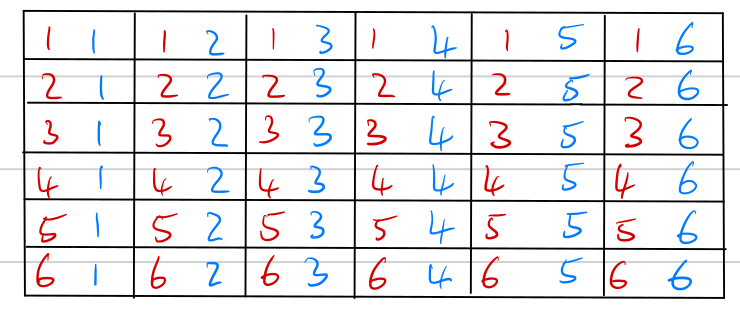
\includegraphics[scale=0.3]{images/state-space-2-dice-rolls}
  \end{center}
  so we can write the sample space as:
  \begin{align*}
    S
    &= \left\{(x,y): x,y\in \left\{1,2,3,4,5,6\right\}\right\}\\
    &= \left\{(1,1), (1,2), \ldots, (6,6)\right\}
  \end{align*}
  The event that the dice are equal is
  \begin{equation*}
    \left[ \text{dice are equal} \right]  = \left\{(1,1), (2,2), (3,3), (4,4), (5,5), (6,6)\right\}
  \end{equation*}
  We could have other events too, like that the dice sum to 3:
  \begin{equation*}
    \left[ \text{dice sum to 4}  \right] = \left\{(1,3),(2,2),(3,1)\right\} 
  \end{equation*}

  % Let's do this for all possible sums of our red and blue dice:
  % \begin{center}
  %   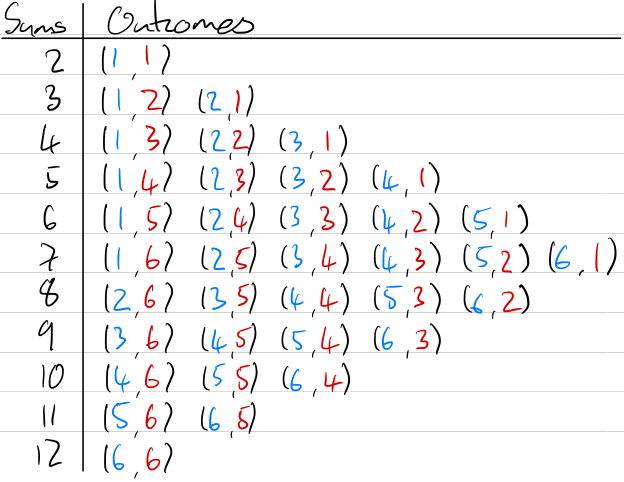
\includegraphics[scale=0.5]{images/sums-events.png}
  % \end{center}
  All of the outcome pairs are equally likely, so we can compute the probabilities of by counting entires
  in the table. Let
  \begin{equation*}
    Z = \text{the sum of the red dice and the blue dice}
  \end{equation*}
  By counting entries in our table, we see that
  \begin{equation*}
    \P\left[Z =  4 \right] = \frac{3}{36}.
  \end{equation*}
  Similarly,
  \begin{equation*}
    \P\left[Z = 7 \right] = \frac{6}{36} = \frac{1}{6}
  \end{equation*}
  and
  \begin{equation*}
    \P\left[Z \leq 5\right] = \frac{10}{36}.
  \end{equation*}
\end{example}

The previous example illustrates the critically imporant idea of \textbf{enumeration:}

\begin{center}
  \colorbox{gray!10}{%
    \begin{minipage}{0.8\textwidth}
      If your sample space is finite and consists of \textit{equally likely outcomes}, then you can
      compute lots of probabilities easily by listing outcomes and counting them. To be prcecise, for any
      event $A$,
      \begin{equation*}
        \P\left[A \right] = \frac{|A|}{|S|}  = \frac{\# \text{ of outcomes in $A$ }}{\# \text{ of outcomes in
            $S$ }}
      \end{equation*}
    \end{minipage}%
  }
\end{center}

I already had you do a bunch of these problems on Monday.




\subsection{Events}

Some observations about events:
\begin{itemize}
  \item Two events $E$ and $F$ are \demph{mutually exclusive} if
  $E\cap F =\emptyset$. This means that $E$ and $F$ cannot both happen at the
  same time.
  \begin{center}
    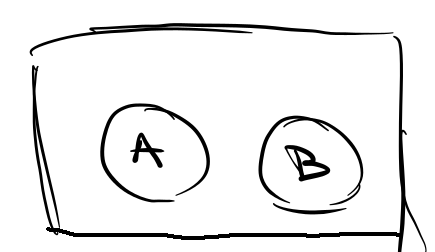
\includegraphics[scale=.4]{images/venn-diagram-disjoint}
  \end{center}

  In the dice example, the events $A$ and $B$ are mutually exclusive, since
  the dice roll cannot be both even and odd. But $A$ and $C$ are not mutually
  exclusive because $A\cap C =\left\{1,3\right\}\neq \emptyset$. If a 1 or a 3
  is rolled, then both $A$ and $C$ occur.

  \item The sample points are \textit{elements} of $S$. The simple events
  are \textit{singleton subsets} of $S$. In the dice example, we have:
  \begin{itemize}
    \item Sample points: 1,2,3,4,5,6.
    \item Simple events:
    $\left\{1\right\},\left\{2\right\},\left\{3\right\},\left\{4\right\},\left\{5\right\},\left\{6\right\}$.
  \end{itemize}
  \item The empty set $\emptyset$ and the whole sample space $S$ are always
  both events: $\emptyset$ is the event ``nothing happens'' and $S$ is the
  event ``something happens''.
  \item If $E$ and $F$ are events, then $E\cap F$ is the event that both $E$
  \textbf{and} $F$ occur:
  \begin{center}
    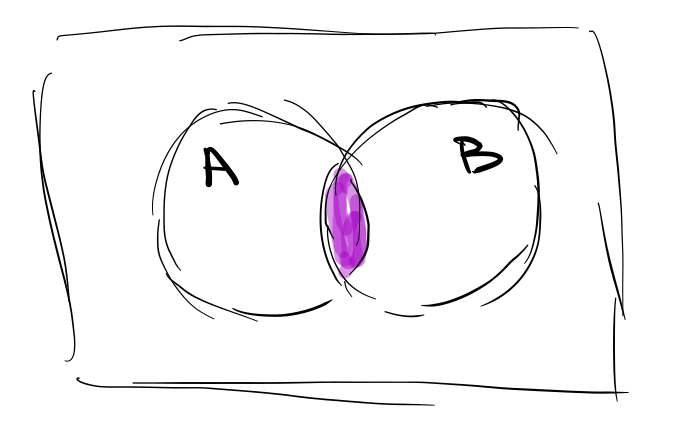
\includegraphics[scale=0.2]{images/venn-diagram-intersection}
  \end{center}
  Here, $E\cap F$ is the \demph{intersection} of $E$ and $F$; that is, $E\cap F$ the set
  of sample points contained in both $E$ and $F$.
\end{itemize}

\newpage
\section{2025-01-16 | Week 01 | Lecture 03}

\begin{center}
  \begin{tcolorbox}[width=0.9\textwidth, colback=white, colframe=black]
    \textit{\textbf{The nexus question of this lecture:} What is the general
      framework for probability (continued)?}

  \end{tcolorbox}
\end{center}

\begin{itemize}
  \item Go over problem 4, parts (b) and (c), and problem 6 on the worksheet.
\end{itemize}



\subsection{Powerball}



\begin{example}[Powerball Lottery]
  \label{ex:powerball-lottery}
  The a ticket for the powerball lottery costs \$2. There are two outcomes:
  \begin{itemize}
    \item You win \$300,000,000.
    \item You don't win any money.
  \end{itemize}
  The probability of winning is approximately $\frac{1}{300,000,000}$. Let $X$ be the net payoff from the
  game, in dollars:
  \begin{itemize}
    \item If you lose, then $X=-2$, since you had to pay \$2 to play the game.
    \item If you win, then your net payoff is $X=299,999,998$. 
  \end{itemize}
  What is the expected value of $X$?
  \begin{align*}
    \E\left[X \right]
    &=\P\left[ \text{win}\right]\cdot (-2) + \P\left[\text{lose} \right]\cdot (299,999,998)\\
    &=\frac{299,999,999}{300,000,000}(-2)+ \frac{1}{300,000,000}(299,999,999)\\
    &=-1.
  \end{align*}
  \textit{Conclusion:} you ``expect'' to lose \$1 every time you play. Similarly, if you play twice, you
  expet to lose \$2. If you play 10 times, you expect to lose \$10. Etc. This property is called
  \textit{linearity} of expectation. 
\end{example}

\subsection{Recap of terminology}

\textit{Recall:} The \demph{sample space} of an experiment is the \textit{set} of all possible
\demph{outcomes}. An \demph{event} is a collection of outcomes. That is,
\begin{equation*}
  \text{an event} = \text{a set of outcomes} = \text{a subset of the sample space $S$.}
\end{equation*}


\begin{example}[Sum 2d4]
  \label{ex:sum-2d4}
  Roll a 4-sided dice twice (this is the \textbf{experiment}). There are 16 possible
  \textbf{outcomes}. The \textbf{sample space} is
  \begin{equation*}
    S = \left\{(x,y): x,y\in \left\{1,2,3,4\right\} \right\},
  \end{equation*}
  which consists of 16 ordered pairs $(x,y)$, the \textbf{sample points}. An
  \textbf{event} is any subset of these.

  We'll give two examples of events.

  Let $X$ be the sum of the two rolls. We can represent $X$ by the following table:
  \begin{equation*}
    \begin{array}{c@{\quad}c|cccc} & \multicolumn{5}{c}{\text{Dice 2}} \\ & &
      1 & 2 & 3 & 4 \\ \cline{2-6}  & 1 & 2 & 3 & 4 & 5 \\ \text{Dice 1} & 2 & 3 & 4 & 5 & 6 \\ & 3 & 4 & 5 & 6 & 7 \\ & 4 & 5 & 6 & 7 & 8 \end{array}
  \end{equation*}

  The event that $X=6$ is:
  \begin{align*}
    [X=6] 
    &= \left\{(1,5), (2,4), (3,3), (4,2), (5,1)\right\}.
  \end{align*}

  Here's another example of an event:
  \begin{align*}
    \left[ X \text{ is even} \right]
    &= \left\{(1,1), (1,3), (2,2), (2,4), (3,1), (3,3), (4,2), (4,4) \right\}.
  \end{align*}

  The \textbf{enumeration principle} says that, when outcomes are equally
  likely, we can compute the probability of an event $E$ by
  \begin{equation*}
    \P\left[E \right] = \frac{|E|}{|S|}.
  \end{equation*}
  So
  \begin{equation*}
    \P\left[X=6 \right] = \frac{3}{16}
  \end{equation*}
  and
  \begin{equation*}
    \P\left[ X\text{ is even} \right] =\frac{8}{16} = \frac{1}{2}.
  \end{equation*}
\end{example}


Since probability theory is formalized in terms of sets, we need to have some intuition about set theory.


\subsection{Understanding the  ``events'' as sets}

% \begin{itemize}
%   \item If $E$ and $F$ are events, then $E\cap F$ is the event that both $E$
%   \textbf{and} $F$ occur:
%   \begin{center}
%     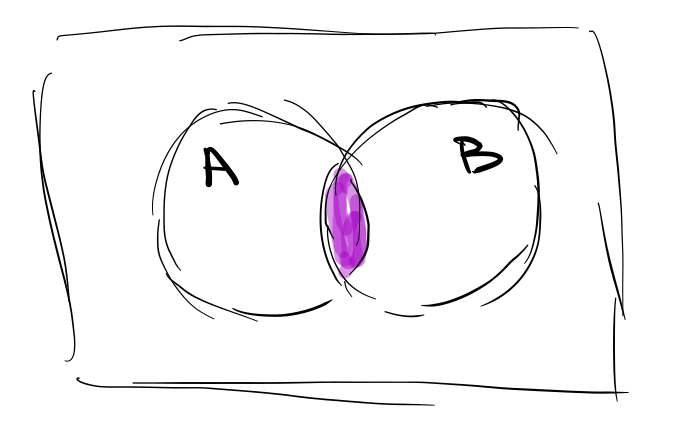
\includegraphics[scale=0.2]{images/venn-diagram-intersection}
%   \end{center}
%   \item If $E$ and $F$ are events, then $E\cup F$ is the event that $E$
%   \textbf{or} $F$ occurs.
%   \begin{center}
%     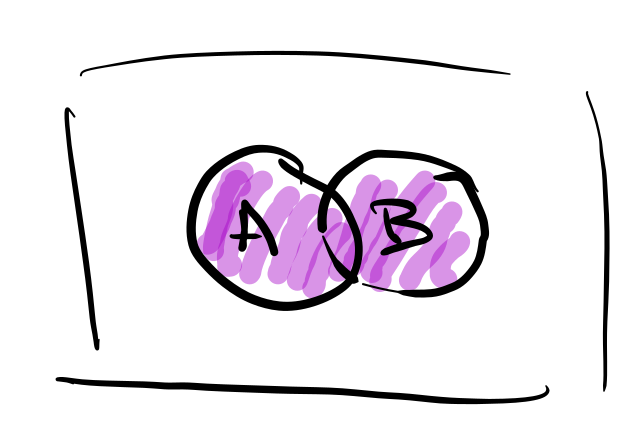
\includegraphics[scale=0.2]{images/venn-diagram-union}
%   \end{center}
%   \item If $A$ is an event, then $A^{c}= S\backslash A$ is the event that $E$
%   does \textbf{not} occur.
%   \begin{center}
%     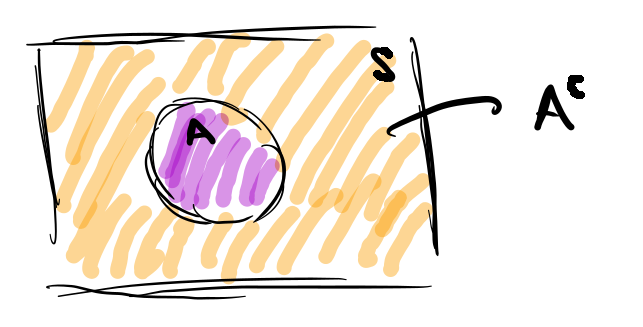
\includegraphics[scale=0.34]{images/venn-diagram-single-event}
%   \end{center}
% \end{itemize}

Let $A$ and $B$ be events. That is, $A$ and $B$ are subsets of $S$.

\begin{itemize}
  \item Suppose $A$ is an event. It's a subset of $S$, like this:
  \begin{center}
    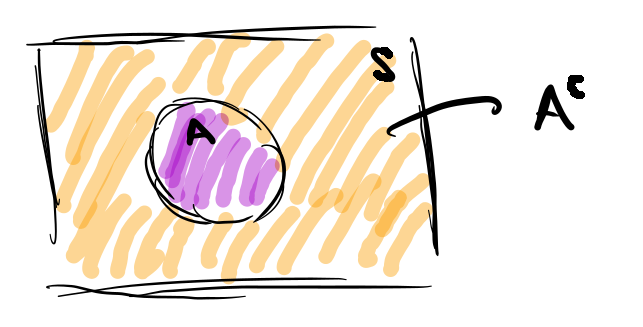
\includegraphics[scale=0.4]{images/venn-diagram-single-event}
  \end{center}
  \item The \demph{complement} of $A$, denoted $A^{c}$ is the set of points
  in $S$ that are \textbf{not} in $A$.

  We interpet $A^{c}$ as the event that $A$ didn't happen.
  
  \item The \demph{union} of $A$ and $B$, denoted $A\cup B$, to denote the set
  of all outcomes that are in $A$ or $B$ this includes outcomes that are in
  both):
  \begin{center}
    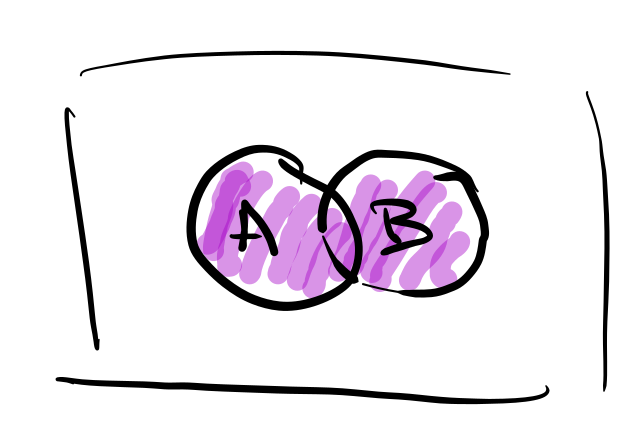
\includegraphics[scale=0.25]{images/venn-diagram-union}
  \end{center}

  We interpret $A\cup B$ as the event that either $A$ or $B$ (or both) occur.
  
  \item The \demph{intersection} of $A$ and $B$, denoted $A\cap B$ is the set
  of points that are contained in both $A$ and $B$:
  \begin{center}
    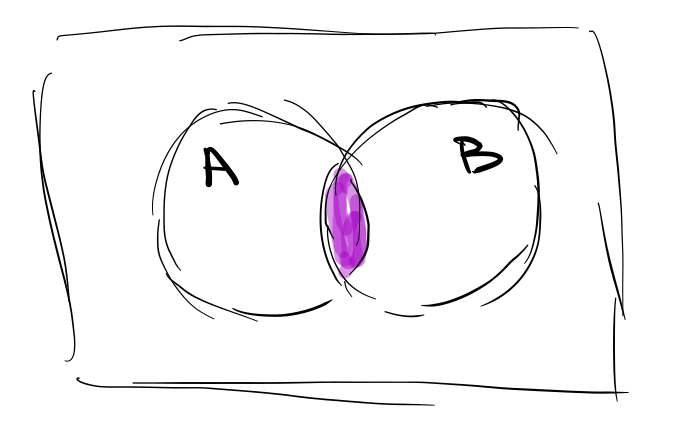
\includegraphics[scale=0.25]{images/venn-diagram-intersection}
  \end{center}

  We interpret $A\cap B$ as the event that $A$ and $B$ both occur.
  
  \item What if $A$ and $B$ don't overlap at all? In that case, their intersection has nothing in it!
  \begin{center}
    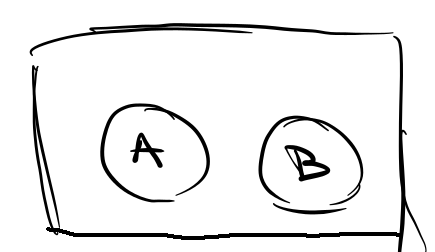
\includegraphics[scale=0.4]{images/venn-diagram-disjoint}
  \end{center}
  In this case, we say that $A\cap B$ is the ``empty set'', which is the set containing no elements. We
  use the symbol $\emptyset$ to represent the empty set; that is,
  \begin{equation*}
    \emptyset := \left\{\right\}
  \end{equation*}
  This is sometimes called the \demph{null event}. If $A\cap B = \emptyset$, then we say that $A$ and $B$
  are \demph{disjoint}. Disjoint events are \demph{mutually exclusive}, in the
  sense that they cannot happen simultaneously.

  For example, when rolling a dice, the following two events are mutually exclusive:
  \begin{equation*}
    [ \text{dice is even}] \quad \text{and} \quad \left[ \text{dice is odd} \right] 
  \end{equation*}
  
  \item An sequence of events $\left\{E_{1},E_{2},\ldots\right\}$ is
  said to be \demph{pairwise disjoint} if and only if
  \begin{equation*}
    E_{i}\cap E_{j} = \emptyset \quad \text{ whenever }i\neq j.
  \end{equation*}
  In other words, none of the events in $E$ ``overlap'' with any other events.
  For an example of this, the experiment from last lecture involving
  repeatedly drawing a ball from an urn with replacement until we get the gold
  ball. Let $X$ be the number of balls we had to draw until we got the gold
  ball. Let
  \begin{equation*}
    E_{n} = \left[ X=n \right] \text{ for }n=1,2,3,\ldots
  \end{equation*}
  Then $\left\{E_{1},E_{2},\ldots\right\}$ is a pairwise disjoint sequence of events.
\end{itemize}


\newpage
\section{2026-01-21 | Week 02 | Lecture 04}
\subsection{Repeated coin flipping}

\begin{example}[Repeated coin flipping]
  \label{ex:cool-coin-flipping-example}
  Consider an experiment in which we flip a coin repeatedly until we get a
  heads. The \textbf{output} of this experiment is \textit{the number of times
    we flipped the coin}.
  
  The sample space of the experiment is
  \begin{equation*}
    S = \left\{1,2,3,4,\ldots\right\}.
  \end{equation*}

  Let $X = (\text{number of coin flips})$. Here, $X$ is a random quantity
  which will vary between experiments. Then
  \begin{equation*}
    \P\left[X = 1 \right] = \P\left[\text{first coin flip was heads} \right] = \frac{1}{2}
  \end{equation*}
  and
  \begin{equation*}
    \P\left[X = 2 \right] 
    = \P\left[\text{first flip was tails and second was heads} \right] 
    = \frac{1}{2}\cdot \frac{1}{2}
    = \frac{1}{4}.
  \end{equation*}
  Similarly,  for any $n=1,2,3,4,\ldots$, we have
  \begin{equation}\label{eq:1}
    \P\left[X=n \right]= \left( \frac{1}{2} \right)^{n} 
  \end{equation}

  \Fl{Question 1:} How many times do we expect to flip the coin? In other words,
  what is $\E\left[X \right]$?

  We use the formula
  \begin{equation*}
    \E\left[X \right] = \sum_{n=1}^{\infty}n \P\left[X=n \right] 
  \end{equation*}
  which gives
  \begin{align*}
    \E\left[X \right] 
    =& \sum_{n=1}^{\infty} n \left( \frac{1}{2} \right)^{n} \\
    =& \frac{1}{2} + 2 \left( \frac{1}{2} \right)^{2}+ 3 \left( \frac{1}{2} \right)^{3}+
       4 \left( \frac{1}{2} \right)^{4}+\ldots \\
    =& \frac{1}{2} +  2\cdot \frac{1}{4}+ 3\cdot \frac{1}{8} + 4\cdot \frac{1}{16}+\ldots\\
    =& \frac{1}{2} + \left(\frac{1}{4}+ \frac{1}{4}\right) + \left(\frac{1}{8} + \frac{1}{8} + \frac{1}{8}\right)
       + \left( \frac{1}{16} + \frac{1}{16} + \frac{1}{16} + \frac{1}{16} \right)  + \ldots\\
    =& \frac{1}{2} + \frac{1}{4} + \frac{1}{8} + \frac{1}{16} + \frac{1}{32} +\ldots\\
     &\phantom{ \frac{1}{2}} + \frac{1}{4} + \frac{1}{8} + \frac{1}{16} + \frac{1}{32}+ \ldots\\
     &\phantom{ \frac{1}{2} + \frac{1}{4}} + \frac{1}{8} + \frac{1}{16} + \frac{1}{32}+ \ldots\\
     &\phantom{ \frac{1}{2} + \frac{1}{4} + \frac{1}{8}} + \frac{1}{16} + \frac{1}{32}+ \ldots\\
     &\phantom{ \frac{1}{2} + \frac{1}{4} + \frac{1}{8} + \frac{1}{16}} + \frac{1}{32}+ \ldots
  \end{align*}
  The first row adds up to $1$ by the geometric series formula (which says that
  $\sum_{n=1}^{\infty}r^{n} = \frac{r}{1-r}$). The second row adds up to $1/2$ (because it's $1/2$ less
  than the first row). The third row adds up to $1/4$. The fourth adds up to $1/8$. etc. So
  \begin{equation*}
    \E\left[X \right] = 1 + \frac{1}{2} + \frac{1}{4}+\frac{1}{8} + \frac{1}{16}+ \ldots
  \end{equation*}
  and applying the geometric series formula again, we see that
  \begin{equation*}
    \E\left[X \right] = 2.
  \end{equation*}
  In other words, we expect to flip the coin twice.
\end{example}

\subsection{The three probability axioms}
\textit{Sections 2.1-2.2 in the textbook.}

\begin{definition}[Probability Measure]
  \label{def:probability-measure}
  A \demph{probability measure} $\P$ is a function which assigns to each event a probability. We denote the
  probability of an event $E$ by
  \begin{equation*}
    \P\left[E \right] \quad \text{or} \quad  \P\left( E\right).
  \end{equation*}
  To be a \demph{probability measure}, $\P$ must satisfy the following three axioms:
  \begin{enumerate}[label=\textbf{A.\arabic*}]
    \item (Nonnegativity) \label{item:probability-axiom-nonnegativity} For every event $E$, we have
    \begin{equation*}
      \P\left[E\right] \geq 0.
    \end{equation*}
    \item (Sum-to-one) \label{item:probability-axiom-total-measure-one} If $S$
    is the whole sample space, then $\P\left[S \right] =1$.
    \item (Countable additivity) \label{item:probability-axiom-countable-additivity} Let
    $E_{1},E_{2},\ldots$ be an infinite sequence of events. If the sequence is pairwise disjoint, then
    \begin{equation*}
      \P\left[E_{1}\cup E_{2}\cup \ldots \right] = \P\left[E_{1} \right]+\P\left[E_{2} \right]+\ldots.
    \end{equation*}
  \end{enumerate}
\end{definition}


Notice that \cref{def:probability-measure} doesn't say how to assign
probabilities. It merely tells us the conditions that probabilities must
satisfy. The first two, \ref{item:probability-axiom-nonnegativity} and
\ref{item:probability-axiom-total-measure-one} seem almost self-evident. The
last one, \ref{item:probability-axiom-countable-additivity}, is more technical
and harder to deciper. The next example gives involves an application of axiom
\ref{item:probability-axiom-countable-additivity}.


\begin{example}[Continuation of  \cref{ex:cool-coin-flipping-example}.]

  Assume the same experiment and notation as
  \cref{ex:cool-coin-flipping-example}.
  
  \Fl{Question 2:} What is the probability that we flip the coin an even
  number of times?

  For each $n=1,2,\ldots$, define the event $E_{n}$ as
  \begin{equation*}
    E_{n} = \left[ X=n \right].
  \end{equation*}
  We want to know the probability that $X$ is even. Observe that
  \begin{equation*}
    \left[ X \text{ is even} \right] = E_{2}\cup E_{4}\cup E_{6}\cup E_{8}\cup\ldots
  \end{equation*}
  We note that the sequence $E_{2},E_{4},E_{6}\ldots $ is pairwise disjoint.
  So we can use \ref{item:probability-axiom-countable-additivity} to compute
  the probability of this event:

  \begin{align*}
    \P\left[X \text{ is even} \right] 
    &= \P\left[E_{2}\cup E_{4}\cup E_{6}\cup E_{8}\cup\ldots \right]\\
    &= \P\left[E_{2} \right] + \P\left[E_{4} \right] + \P\left[E_{6} \right] + \P\left[E_{8} \right] +
      \ldots &&\text{(by \ref{item:probability-axiom-countable-additivity}) }\\
    &= \left( \frac{1}{2} \right)^{2}+\left( \frac{1}{2} \right)^{4}+\left( \frac{1}{2} \right)^{6}+\left(
      \frac{1}{2} \right)^{8}+\ldots &&\text{(by \cref{eq:1}) }\\
    &= \frac{1}{4}+\left( \frac{1}{4} \right)^{2}  + \left( \frac{1}{4} \right)^{3} + \left( \frac{1}{4} \right)^{4}+\ldots\\  
    &= \frac{\frac{1}{4}}{1-\frac{1}{4}} &&\text{by geometric series formula $\sum_{n=1}^{\infty}r^{n} = \frac{r}{1-r} $ }\\
    &= \frac{1}{3}. 
  \end{align*}
  So the probability that you flip the coin an \textit{even} number of times is only $1/3$. 
\end{example}

\subsection{Inclusion-exclusion principle}
\begin{theorem}[Inclusion-Exclusion Prinicple]
  \label{thm:inclusion-exclusion-principle}
  If $A$ and $B$ are events, then
  \begin{equation*}
    \P\left[A\cup B \right] = \P\left[A \right]+\P\left[B \right]- \P\left[A\cap B \right]
  \end{equation*}
  In particular, if $A$ and $B$ are distjoint, then
  \begin{equation*}
    \P\left[A\cup B \right]= \P\left[A \right]+\P\left[B \right].
  \end{equation*}
\end{theorem}
\begin{proof}[Idea of proof]
  $\P\left[A\cup B \right]$ is the area of the red-shaded region:
  \begin{center}
    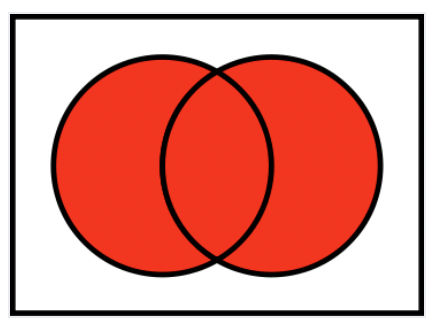
\includegraphics[scale=.5]{images/venn-diagram-union-2}
  \end{center}
  Compare with $\P\left[A \right]+\P\left[B \right]- \P\left[A\cap B \right]$:
  \begin{center}
    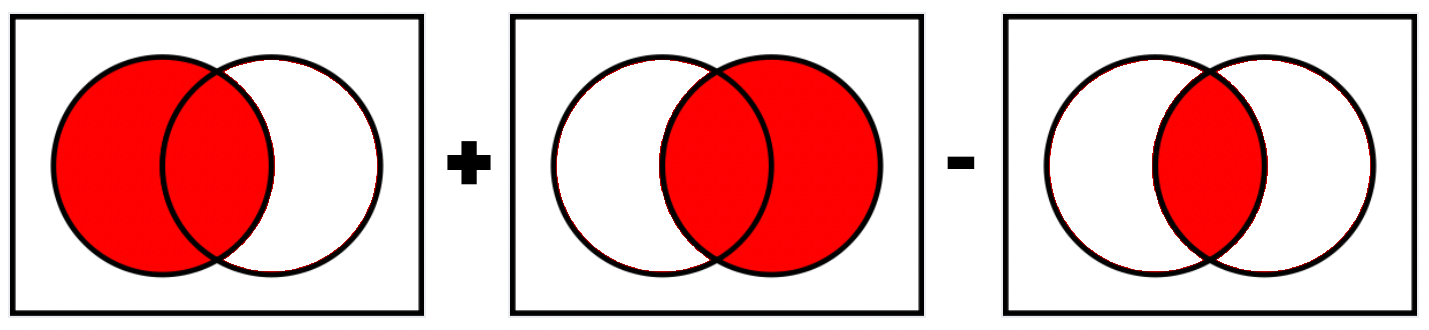
\includegraphics[scale=.5]{images/inclusion-exclusion}
  \end{center}
\end{proof}


\newpage
\section{2026-01-23 | Week 02 | Lecture 05}

\subsection{St. Petersburg Paradox}

The game is the following: repeatedly flip a coin until you get heads. You win $2^{n}$ dollars, where $n$ is
the number of coin flips. How much would you be willing to pay to play this game????

Let $X$ be your (random) payoff. The sample space of $X$ is
\begin{equation*}
  S = \left\{2,4,8,16,32,\ldots\right\}.
\end{equation*}
What is the expected value of $X$?

\begin{align*}
  \E\left[X \right] 
  &= \sum_{x} x \P\left[X=x \right]\\
  &= 2\P\left[X=2 \right]+ 4 \P\left[X=4 \right] + 8\P\left[X=8 \right] + 16 \P\left[X=16 \right]+\ldots\\
\end{align*}
Next, we observe that $\P\left[X=2^{k} \right] = \frac{1}{2^{k}}$ for all
$k =1,2,\ldots$. Plugging these probabilities in, we get

\begin{equation*}
  \E\left[X \right] = 1+1+1+1+1+\ldots   = +\infty.
\end{equation*}
The expected value of playing this game is positive infinity!!!!! N matter how
much you pay to play this game, you will eventually make money if you play
enough times.

\subsection{What is probability, continued}


\begin{definition}[Probability Measure]
  \label{def:probability-measure}
  A \demph{probability measure} $\P$ is a function which assigns to each event a probability. We denote the
  probability of an event $E$ by
  \begin{equation*}
    \P\left[E \right] \quad \text{or} \quad  \P\left( E\right).
  \end{equation*}
  To be a \demph{probability measure}, $\P$ must satisfy the following three axioms:
  \begin{enumerate}[label=\textbf{A.\arabic*}]
    \item (Nonnegativity) \label{item:probability-axiom-nonnegativity} For every event $E$, we have
    \begin{equation*}
      \P\left[E\right] \geq 0.
    \end{equation*}
    \item (Sum-to-one) \label{item:probability-axiom-total-measure-one} If $S$
    is the whole sample space, then $\P\left[S \right] =1$.
    \item (Countable additivity) \label{item:probability-axiom-countable-additivity} Let
    $E_{1},E_{2},\ldots$ be an infinite sequence of events. If the sequence is pairwise disjoint, then
    \begin{equation*}
      \P\left[E_{1}\cup E_{2}\cup \ldots \right] = \P\left[E_{1} \right]+\P\left[E_{2} \right]+\ldots.
    \end{equation*}
  \end{enumerate}
\end{definition}


\begin{proposition}[Basic properties of probability measure]
  \label{prop:some-deductions-from-axioms}
  \begin{enumerate}[label=\rm{(\roman*.)}]
    \item []
    \item (The null event has probability zero) \label{item:empty-set-has-prob-zero}
    $\P\left[\emptyset \right] = 0$
    \item (Finite additivity) \label{item:finite-additivity} If
    $E_{1},\ldots,E_{n}$ are pairwise disjoint, then
    \begin{equation*}
      \P\left[E_{1}\cup E_{2}\cup\ldots\cup E_{n} \right] 
      = \P\left[E_{1} \right]+\P\left[E_{2} \right]+\ldots+\P\left[E_{n} \right]
    \end{equation*}
    \item (``With probability one, an event $E$ either does occur or doesn't'') \label{item:complements} $\P\left[E^{c} \right] = 1-\P\left[E \right]$
    \item (Excision Property) \label{item:excision-property} If $A,B$ are events and $A\subseteq B$, then
    \begin{equation*}
      \P\left[B\backslash A \right] = \P\left[B \right] - \P\left[A \right].
    \end{equation*}
    \item (``The particular is less likely than the general'') \label{item:subsets} If $A,B$ are events and $A\subseteq B$, then
    $\P\left[ A\right] \leq \P\left[B \right]$
    \item (``Probabilities are between 0 and 1'') \label{item:probabilities-are-in-unit-interval} For any event $E$,  $\P\left[E \right]\in [0,1]$
  \end{enumerate}
\end{proposition}
% \begin{proof}[Proof of \cref{prop:some-deductions-from-axioms}]
%   First we will prove \ref{item:empty-set-has-prob-zero}. Let $E_{i}=\emptyset$ for all $i=1,2,3,...$.
%   Then
%   \begin{itemize}
%     \item $\left\{E_{1},E_{2},\ldots\right\}$ is a pairwise disjoint sequence.
%     \item If $E_{1}\cup E_{2}\cup\ldots = \emptyset$.
%   \end{itemize}
%   Therefore,
%   \begin{align*}
%     \P\left[\emptyset \right] 
%     &= \P\left[E_{1}\cup E_{2}\cup\ldots \right]\\
%     &= \P\left[E_{1} \right]+ \P\left[E_{2} \right]+\ldots
%     &&\text{by \ref{item:probability-axiom-countable-additivity} }\\
%     &= \P\left[\emptyset \right]+ \P\left[\emptyset \right]+\ldots.
%   \end{align*}
%   This equation implies $\P\left[\emptyset \right] = 0$. We have now proved
%   \ref{item:empty-set-has-prob-zero}.


%   Next we prove \ref{item:finite-additivity}. Let $E_{1},\ldots,E_{n}$ be a finite sequence of events
%   which are pairwise disjoint.  Then expand the sequence by taking $E_{i} = \emptyset$ for all $i\in
%   \left\{n+1,n+2,\ldots\right\}$. Then by \ref{item:probability-axiom-countable-additivity},
%   \begin{align*}
%     \P\left[\bigcup_{i=1}^{n}E_{i} \right]
%     &= \sum_{i=1}^{\infty} \P\left[E_{i} \right] \\
%     &= \P\left[E_{1} \right] + \ldots \P\left[E_{n} \right] +
%       \underbrace{\P\left[\emptyset \right] + \P\left[\emptyset \right]+\ldots}
%       _{=0\text{ by \cref{prop:some-deductions-from-axioms} \ref{item:empty-set-has-prob-zero}}}\\
%     &=\P\left[E_{1} \right] + \ldots \P\left[E_{n} \right].
%   \end{align*}

%   Next we prove \ref{item:complements}. Let $E$ be any event. Then
%   \begin{align*}
%     1 
%     &= \P\left[S \right]  &&\text{by \ref{item:probability-axiom-total-measure-one} }\\
%     &= \P\left[ E\cup E^{c}\right] &&\text{since }S = E\cup E^{c}\\
%     &= \P\left[E \right]+ \P\left[E^{c} \right]
%                           &&\text{by
%                              \cref{prop:some-deductions-from-axioms}~\ref{item:finite-additivity},
%                              since $E\cap E^{c}=\emptyset$.}
%   \end{align*}
%   This proves \ref{item:complements}.

%   Next we prove \ref{item:excision-property}. Observe that
%   \begin{align*}
%     B 
%     &= (B\cap A) \cup (B\cap A^{c})\\
%     &= A \cup B\cap A^{c} &&\text{since $A\subseteq B$.}
%   \end{align*}
%   This is a disjoint union. Therefore by \ref{item:finite-additivity},
%   \begin{align*}
%     \P\left[B \right] 
%     &= \P\left[A \right] + \P\left[B\cap A^{c} \right]\\
%     &= \P\left[A \right] + \P\left[B\backslash A \right].
%   \end{align*}
%   Rearranging terms proves \ref{item:complements}. 
%   Next we prove \ref{item:subsets}. Assume $A\subseteq B$. Then by \ref{item:excision-property},
%   \begin{equation*}
%     \P\left[B\backslash A \right] = \P\left[B \right] - \P\left[A \right]
%   \end{equation*}
%   Moreover, by \ref{item:probability-axiom-nonnegativity}, $\P\left[B\backslash A \right] \geq 0$.
%   Hence
%   \begin{equation*}
%     0 \leq  \P\left[B \right] - \P\left[A \right]
%   \end{equation*}
%   and this implies \ref{item:subsets}.
  
%   Finally, we will show \ref{item:probabilities-are-in-unit-interval}. Let $E$ be an event. Then
%   \begin{align*}
%     0 
%     &\leq \P\left[E \right]  &&\text{by \ref{item:probability-axiom-nonnegativity} }\\
%     &\leq  \P\left[S \right] &&\text{by \ref{item:subsets} }\\
%     &=1 &&\text{by \ref{item:probability-axiom-total-measure-one}. }
%   \end{align*}
% \end{proof}


\begin{proposition}[De Morgan's Laws]
  \label{prop:de-morgans-laws}
  The following equalities hold:
  \begin{equation*}
    \left( A\cup B \right)^{c} = A^{c}\cap B^{c}
    \quad \text{and} \quad 
    \left( A\cap B \right)^{c} = A^{c}\cap B^{c}.
  \end{equation*}
\end{proposition}
\begin{proof}
  Draw a picture.
\end{proof}



\newpage
\section{2026-01-26 | Week 03 | Lecture 06}

\textit{This lecture is based on section 2.3 in the textbook.}

There are three main counting principles we'll look at:
\begin{itemize}
  \item multiplication principle
  \item permutation principle
  \item combination principle
\end{itemize}

\subsection{Multiplication principle}



\begin{example}
  A man has 3 shirts and two ties. How many ways
  can he dress himself?
  \begin{center}
    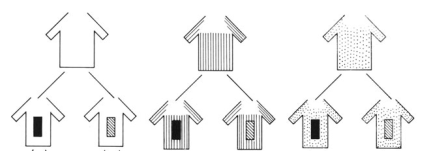
\includegraphics[scale=.6]{images/chung-ties}
  \end{center}
  We can schematize this as three shirts $s_{1},s_{2},s_{3}$ and two ties
  $t_{1},t_{2}$, in which case the possible outfits are:
  \begin{align*}
    &(s_{1},t_{1})\  (s_{2},t_{1})\  (s_{3},t_{1})\\
    &(s_{1},t_{2})\  (s_{2},t_{2})\  (s_{3},t_{2})
  \end{align*}
  Of course, we don't need to write $s$ and $t$; it is enough to write
  \begin{align*}
    &(1,1)\ (2,1)\ (3,1)\\
    &(1,2)\ (2,2)\ (3,2)
  \end{align*}
  where the first slot is ``shirt'' and the second is ``tie''. Thus the
  methematical way to name the collection of outfits is the set of all ordered
  couples $(a,b)$ with $a=1,2$ and $b=1,2,3$. So you can see the total number
  of outfits is $2\times 3 = 6$.

  In general we can talk about ordered $k$-tuples $(a_{1},\ldots,a_{k})$,
  where for each $j$ from $1$ to $k$, the symbol $a_{j}$ is the assignment
  (choice) for the  $j^{\rm th}$ slot and it may be denoted by a numeral
  between $1$ and $n_{j}$. In our example, $k=2$ and $n_{1}=3$ and $n_{2}=2$.


  If the man also have two pairs of shoes, we can add a third slot for
  ``shoes'', so the question is asking to count the number of elements in the
  set
  \begin{equation*}
    \left\{ (a_{1},a_{2},a_{3}): a_{1}\in \left\{1,2,3\right\} , a_{2},a_{3}\in \left\{1,2\right\} \right\}
  \end{equation*}
  In this case, $n_{1} = 3$, $n_{2} = 2$ and $n_{3}=2$, so the number of
  outfits is
  \begin{equation*}
    n_{1}n_{2}n_{3} = 3\cdot2\cdot2 = 12,
  \end{equation*}
  which is shown in the following picture:
  \begin{center}
    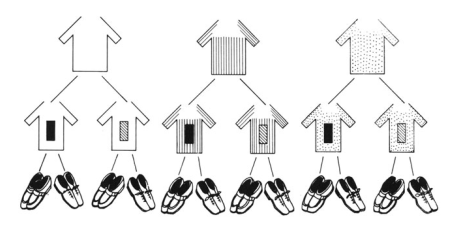
\includegraphics[scale=.3]{images/chung-shoes}
  \end{center}
\end{example}


In this example, we've used the ``multiplication principle''. Let's state this
principle formally now. To do so, we need the following definition:

\begin{definition}[k-tuple]
  \label{def:k-tuple}
  A \demph{$k$-tuple} is an ordered list of $k$ objects. 
\end{definition}

For example, $(1,2,5,4) $ and $(3,3,5,4)$ are both examples of $4$-tuples.
Note that repeats are allowed. 



\begin{theorem}[Multiplication Principle]
  \label{thm:multiplication-principle}
  Suppose $S$ consist of $k$-tuples and there are $n_{1}$ choices for the first element, $n_{2}$ choices
  for the second, etc. Then there are
  \begin{equation*}
    n_{1}\times n_{2}\times \cdots \times n_{k}
  \end{equation*}
  possible $k$-tuples.
\end{theorem}


\begin{example}[Application of the multiplication principle to probability]
  Consider an experiment in which we roll a dice 5 times in a row. One
  possible outcome is
  \begin{equation*}
    (1,4,6,4,4).
  \end{equation*}
  This is an ordered list with five entries, i.e., a 5-tuple.

  
  \Fl{Problem 1:} What is the sample space? How many elements does it have?

  \begin{itemize}
    \item there are 6 choices for the first entry
    \item 6 choices for the second entry
    \item[] $\vdots $ 
    \item 6 choices for the fifth entry
  \end{itemize}
  so the number of possible outcomes is
  \begin{equation*}
    6\times 6 \times 6 \times 6 \times 6 = 6^{5 } = 7776.
  \end{equation*}

  
  \Fl{Problem 2:} Let $E = \left[ \text{All 5 dice are less than or equal to 3} \right]$. What is
  $\P\left[E \right]?$

  By the enumeration principle,
  \begin{equation*}
    \P\left[E \right] = \frac{|E|}{|S|} = \frac{\text{\# ways that all dice are $\leq 3$ }}{7776}
  \end{equation*}
  now we use again the multiplication principle to count the $k$-tuples with
  all entries less than $3$:
  \begin{equation*}
    3\times 3 \times 3 \times 3 \times 3 = 3^{5} = 243
  \end{equation*}
  So
  \begin{equation*}
    \P\left[E \right] = \frac{243}{7776} = \frac{1}{32}
  \end{equation*}
\end{example}



\subsection{Permutations and combinations}

\begin{example}
  How many ways are there to order the $4$ letters $A,B,C,D$?

  Use the multiplication principle
  \begin{equation*}
    4\times 3 \times 2 \times 1
  \end{equation*}
\end{example}

\begin{proposition}[Counting permutations]
  \label{prop:counting-permutations}
  The total number of ways to order $n$ distinct objects is
  \begin{equation*}
    n! = n \times (n-1)\times(n-2)\times\cdots\times 2 \times 1.
  \end{equation*}
  (Note that we define $0! = 1.$)
\end{proposition}


\begin{definition}[permutation and combination]
  A \demph{set} is an \textit{unordered} collection of elements, all of which are \textit{distinct.}
  \begin{itemize}
    \item $\left\{1,2,4,5,3\right\}$ is a set
    \item $\left\{1,1,2,4,5,3\right\}$ is not a set
  \end{itemize}

  A \demph{permutation} is an ordered subset. An unordered subset is called a \demph{combination}.
\end{definition}


\newpage
\section{2026-01-28 | Week 03 | Lecture 07}
\textit{This lecture is based on section 2.3 in the textbook.}

\subsection{Review of multiplication principle}
\begin{definition}[k-tuple]
  \label{def:k-tuple}
  A \demph{$k$-tuple} is an ordered list of $k$ objects. 
\end{definition}


\begin{theorem}[Multiplication Principle]
  \label{thm:multiplication-principle}
  Suppose $S$ consist of $k$-tuples and there are $n_{1}$ choices for the first element, $n_{2}$ choices
  for the second, etc. Then there are
  \begin{equation*}
    n_{1}\times n_{2}\times \cdots \times n_{k}
  \end{equation*}
  possible $k$-tuples.
\end{theorem}

\subsection{The permutation principle and the combination principle}


\begin{proposition}[Counting permutations]
  The total number of ways to order $n$ distinct objects is
  \begin{equation*}
    n! = n \times (n-1)\times(n-2)\times\cdots\times 2 \times 1.
  \end{equation*}
  (Note that we define $0! = 1.$)
\end{proposition}


\begin{definition}
  A \demph{set} is an \textit{unordered} collection of elements, all of which
  are \textit{distinct.} A \demph{permutation} is an ordered subset. An
  unordered subset is called a \demph{combination}.
\end{definition}



\begin{theorem}[The permutation principle]
  \label{thm:permutation-principle}
  The number of permutations of size $k$ that can be formed from $n$ objects
  is
  \begin{equation*}
    (n)_{k} := n\cdot (n-1)\cdot (n-2)\cdots (n-k+1) = \frac{n!}{(n-k)!}.
  \end{equation*}
  There are $k$ terms in this product. (The book uses the notation $P_{k,n}$
  instead of $(n)_{k}$.) 
\end{theorem}
\begin{proof}
  Suppose our $n$ objects are $n$ balls in an urn, labeled $1,\ldots,n$. We
  draw $n$ balls sequentially, each ball drawn is left out of the urn. The
  number permutations is the number of ways that $k$ balls can be drawn out of
  the urn. We are dealing with ordered $k$-tuples
  \begin{equation*}
    (a_{1},\ldots,a_{k})
  \end{equation*}
  where $a_{1},\ldots,a_{k}\in \left\{1,\ldots,n\right\}$ are integers between
  $1$ and $n$ that must all be different. (Obviously, $k \leq n$ since there
  are $n$ balls in the urn and we seek to draw out $k$ of them).

  For the first ball, we have $n$ choices. For the second ball we have $n-1$
  choice (since there remain only $n-1$ balls in the urn after our first
  draw). For the third ball we have $n-2$ choices, and so forth. By the
  $k^{\rm th}$ ball (our final draw), there are $n-k+1$ balls to choose from
  in the urn.

  Therefore, by the multiplication principle, 
  \begin{equation*}
    \text{the number of permutations} = n\cdot(n-1)\cdot(n-2)\cdots (n-k+1) = \frac{n!}{(n-k)!}.
  \end{equation*}
\end{proof}

\begin{theorem}[The combination principle]
  \label{thm:combination-principle}
  Let $S$ be a set with $n$ elements. The number of (unordered) subsets of size $k$ is
  \begin{equation*}
    {n\choose k} =  \frac{n!}{k!(n-k)!}
  \end{equation*} 
\end{theorem}

\begin{proof}
  To understand why the formula of \cref{thm:combination-principle} is
  correct, we begin by making two observations:
  \begin{itemize}
    \item \textbf{Observation 1.} For every unordered subset of size $k$,
    there are $k!$ ways to order it by \cref{prop:counting-permutations}.

    Therefore the following equation holds:
    \begin{equation*}
      k! \times \text{(number of unordered subsets of size $k$)}
      =
      \text{(number of ordered subsets of size $k$)}
    \end{equation*}
    
    \item \textbf{Observation 2.} The permutation principle
    (\cref{thm:permutation-principle}) tells us that
    \begin{equation*}
      \text{(number of ordered subsets of size $k$)}=\frac{n!}{(n-k)!}.
    \end{equation*}
  \end{itemize}

  We now put these two observations together. Let $X$ and $Y$ be the following
  quantities:
  \begin{align*}
    X &= \text{(number of ordered subsets of size $k$)}\\
    Y &= \text{(number of unordered subsets of size $k$)}.
  \end{align*}
  Then
  \begin{align*}
    k!\cdot Y
    &= X &&\text{by Observation 1}\\
    &= \frac{n!}{(n-k)!} &&\text{by Observation 2}
  \end{align*}
  Dividing both sides by $k!$ gives
  \begin{equation*}
    Y = \frac{n!}{k!(n-k)!},
  \end{equation*}
  and this proves \cref{thm:combination-principle}.
\end{proof}



\subsection{Examples of the three combinatorial principles}

\begin{example}
  A dessert company has 32 distinct desserts on its menu: 6 types of pie, 9
  types of cake, and 17 flavors of ice cream.
  \begin{enumerate}[(a)]
    \item \textbf{Question:} After purchasing 4 different desserts, a customer decides he will
    eat them all in a row, and he cares about the order in which he eats them.
    How many different ways can he eat his 4 desserts?

    \textbf{Solution:} Here we are counting the number of ways to order
    set of four objects. This number is $4!$ by
    \cref{prop:counting-permutations}.
    
    \item \textbf{Question:} How many ways are there for the customer to choose
    four desserts and then eat them in a particular order of his choice?

    \textbf{Solution 1:} By the combination principle, there are ${32\choose 4}$
    combinations of desserts that the customer could choose. Moreover, by part
    (a), for each combination of 4 desserts, he can order them $4!$ ways.
    Therefore by the multiplication principle, there are
    \begin{equation*}
      {32\choose 4} \times 4! = 32\cdot 31\cdot 30\cdot 29
    \end{equation*}
    ways that the customer could choose and then eat four desserts.

    \textbf{Solution 2:} Another solution would be to note that we want to
    count the number of permutations of size $k=4$ from a set of $n=32$
    distinct objects. (Think: the customer is selecting 4 desserts from an urn
    with 32 distinct desserts in it). By the permutation principle, this
    number is
    \begin{equation*}
      (32)_{4} = 32\cdot 31\cdot30 \cdot29
    \end{equation*}
    which agrees with our answer from solution 1.

    \item \textbf{Question:} If 9 desserts are randomly selected, how many ways
    are there to obtain 3 deserts of each type (pie, cake, and ice cream)?

    \fl{Solution:} For pie, there are ${6\choose 3}$ combinations possible.
    For cake, there are ${9\choose 3}$ combinations possible, and for ice
    cream, there are ${17\choose 3}$.

    By the multiplication principle, there are
    \begin{equation*}
      {6\choose 3}\times {9\choose 3}\times {17\choose 3}
    \end{equation*}
    ways to simultaneously select 3 pies, 3 cakes, and 3 ice cream flavors.
  \end{enumerate}
\end{example}
\newpage


\section{2025-01-30 | Week 03 | Lecture 08}

\textit{This lecture is based on sections 2.3 and 2.4 in the textbook.}


\subsection{Applications of the 3 combinatorial principles}
\begin{example}
  Let $S = \left\{1,2,3,4,5,6\right\}$. How many unordered subsets (i.e.,
  combinations) of size 2 are there?

  \begin{equation*}
    {6\choose 2} = \frac{6!}{2! \cdot 4!} = \frac{6\cdot5\cdot4\cdot3\cdot2\cdot1}{\left(2\cdot1\right) \cdot \left(4\cdot3\cdot2\cdot1\right)} = \frac{6\cdot5}{2} = 15.
  \end{equation*}
  The fiften combinations are
  \begin{align*}
    \left\{1,2\right\}, \left\{1,3\right\}, \left\{1,4\right\}, \left\{1,5\right\}, &\left\{1,6\right\} \\
    \left\{2,3\right\}, \left\{2,4\right\}, \left\{2,5\right\}, &\left\{2,6\right\} \\
    \left\{3,4\right\}, \left\{3,5\right\}, &\left\{3,6\right\} \\
    \left\{4,5\right\}, &\left\{4,6\right\} \\
    & \left\{5,6\right\}
  \end{align*}
  note that the order doesn't matter, i.e., $\left\{2,1\right\}=\left\{1,2\right\}$ so this just counts
  as one, not two.

\end{example}

\begin{example}[Poker]
  A poker hand consist of 5 randomly chosen cards from a
  standard 52-card deck.
  \begin{center}
    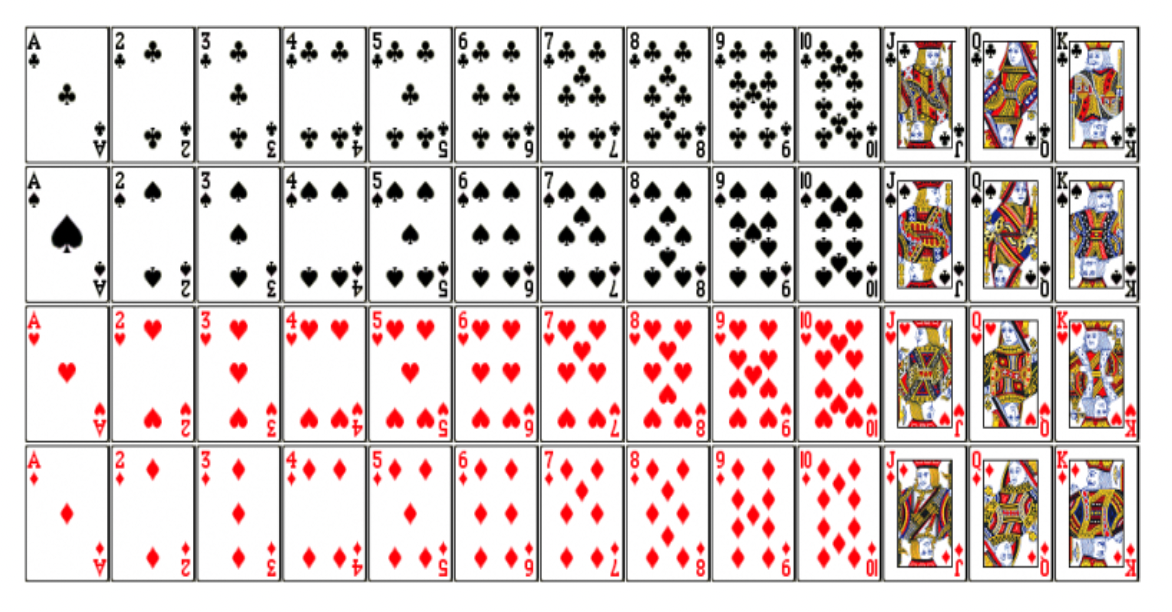
\includegraphics[scale=0.3]{images/52-card-deck}
  \end{center}
  \fl{Some questions about poker hands:}
  \begin{enumerate}
    \item How many distinct poker hands are there?

    \begin{equation*}
      {52\choose 5} = \frac{52!}{5!\cdot47!} = 2,598,960
    \end{equation*}
    \item A \textbf{flush} occurs when all five cards are the same suit. How
    many ways are there to get a flush?
    \begin{equation*}
      4 \times {13\choose 5} 
      = 4\cdot \frac{13!}{5! 8!} 
      = 4\cdot\frac{13\cdot 12\cdot 11 \cdot 10 \cdot 9}{5\cdot4\cdot3\cdot2\cdot1} 
      = 5148
    \end{equation*}

    The 4 is to choose a suit. Then we choose 5 out of 13 cards in that suit.
    \item What's the probability of getting a flush?

    To answer this, we use the enumeration principle:
    \begin{equation*}
      \frac{{4\choose 1}\times {13\choose 5}}{{52\choose 5}} = \frac{5,148}{2,598,960} \approx 0.002
    \end{equation*}

    In other words, the probability of a flush is pretty low: about $0.2\%$.
  \end{enumerate}
\end{example}

\subsection{Introduction to craps}
Craps is a dice-rolling game in which a player, known as the shooter, rolls a
pair of 6-sided dice. The shooter wins, loses or re-rolls depending on what
happens.

Here's a set of rules for the shooter:
\begin{enumerate} 
  \item You roll two dice and add them up.
  \begin{itemize}
    \item If the sum is $2,3$, or $12$, you lose (``craps'')
    \item If you roll $7$ or $11$, then you win  (``natural'')
    \item Otherwise you establish ``point'', which is whatever number you got.
  \end{itemize}
  \item If you established point, then you must keep rolling until one of two events occurs:
  \begin{itemize}
    \item You roll a 7: you lose
    \item You roll your ``point'' number: you win.
  \end{itemize}
\end{enumerate}


Tallying the results, we saw that shooters won about 50\% of the time. Is this a fair game? We will set
out to answer this question. To do so, we'll need to introduce some new ideas. A key idea is that of
conditional probability:

\subsection{Conditional probability}
\textit{This section is based on section 2.4 in the text.}



\begin{definition}[Conditional Probability]
  \label{def:conditional-probability}
  Let $A,B$ be events, and assume that $\P\left[A\right]>0$. Then the \demph{conditional probability of
    $B$, given $A$}, denoted $\P\left[B\mid A \right]$, is given by the formula
  \begin{equation*}
    \P\left[B\mid A \right] := \frac{\P\left[A\cap B \right]}{\P\left[A \right]}.
  \end{equation*}
\end{definition}

\newpage
\section{2026-02-02 | Week 04 | Lecture 09}

\subsection{Conditional probability}
\textit{This section is based on section 2.4 in the text.}

\begin{definition}[Conditional probability]
  \label{def:conditional-probability}
  Let $A,B$ be events, and assume that $\P\left[A\right]>0$. Then the
  \demph{conditional probability of $B$, given $A$}, denoted
  $\P\left[B\mid A \right]$, is given by the formula
  \begin{equation*}
    \P\left[B\mid A \right] = \frac{\P\left[A\cap B \right]}{\P\left[A \right]}.
  \end{equation*}
\end{definition}

\fl{Interpretation:} $\P\left[A\mid B \right]$ is the probability of $A$ when
we know that event $B$ happened.

\Fl{Multiplication rule:} $\P\left[A\cap B \right] = \P\left[B\mid A \right] \P\left[A \right]$

\begin{definition}
  \label{def:positive-relationship}
  We say that there exists a \demph{positive relationship} between events $A$
  and $B$ if
  \begin{equation*}
    \P\left[B\mid A \right]> \P\left[B \right],
  \end{equation*}
  and a \demph{negative relationship} if
  \begin{equation*}
    \P\left[B\mid A \right]< \P\left[B \right].
  \end{equation*}
\end{definition}
 

\begin{itemize}
  \item Smoking and getting lung canger have a positive relationship: if you
  know someone is a smoker $(A)$, then the probability that they get lung
  cancer $(B)$ is higher than if you didn't know they were a smoker.
  
  % \item The idea is that if we know that event $A$ has occured, then the
  % sample space becomes $A$, and the new event is $A\cap B$.
\end{itemize}


\begin{example}[Conditional probability]
  I roll a dice behind a screen. I tell you that I rolled an even number. What's the probability that the
  dice roll is a $4$ or a $6$?

  \Fl{Solution:} We have $S = \left\{1,2,3,4,5,6\right\}$, $A= \left\{2,4,6\right\}$,
  $B= \left\{4,6\right\}$. We want to compute $\P\left[B\mid A \right]$. By \cref{def:conditional-probability},
  \begin{equation*}
    \P\left[B\mid A \right] 
    = \frac{\P\left[AB \right]}{\P\left[A \right]} 
    = \frac{2/6}{1/2} 
    = \frac{2}{3}.
  \end{equation*}
  Put differently, we have three outcomes in $A$, which are all equally likely. Two of them (4 and 6)
  mean that event $B$ occurs. So by the enumeration principle, the probability is $2/3$.
\end{example}




\begin{example}[Similar to examples 2.27 and 2.28 in the textbook]
  A vampire goes to the blood bank looking to find some type O+ blood (the most delicious type). He finds
  4 unlabeled bags of blood. Only one of the bags is O+, but the vampire doesn't know which one, so he
  resorts to taste-testing to find the O+ bag.
  \begin{enumerate}[(a),itemsep=0em]
    \item What is the probability that he must test at least 3 bags to find
    the desired type?

    \fl{Solution:} Let $X$ be the number of tested bags. We
    want to find $\P\left[X \geq 3\right]$. Let
    \begin{equation*}
      A = \left[ \text{first bag isn't O+} \right]
      \quad \text{and} \quad B = \left[ \text{second bag isn't O+} \right]
    \end{equation*}
    \begin{align*}
      \P\left[ X \geq 3\right] 
      &= \P\left[A\cap B \right]\\
      &= \P\left[A \right] \P\left[B\mid A \right]\\
      &= \frac{3}{4}\cdot \frac{2}{3}\\
      &= \frac{1}{2}.
    \end{align*}
    \item What's the probability that he must test exactly $3$ bags?

    \fl{Solution:} We want $\P\left[X=3 \right]=\P\left[\text{first bag isn't
        O+ $\cap$ second bag isn't O+ $\cap$ third bag is O+} \right]$.

    \begin{align*}
      \P\left[X=3 \right] 
      &= \P\left[\text{third is}\mid  \text{first isn't} \cap
        \text{second isn't}  \right] \times \P\left[\text{second isn't}\mid \text{first isn't} \right] \cdot
        \P\left[\text{first isn't} \right]\\
      &= \frac{1}{2}\cdot \frac{2}{3}\cdot \frac{3}{4}\\
      &= \frac{1}{4}
    \end{align*}

    Here we have used the following multiplication rule:
    \begin{align*}
      \P\left[A\cap B\cap C \right] 
      &= \P\left[ C\mid A\cap B\right] \P\left[A\cap B \right]\\
      &= \P\left[ C\mid A\cap B\right] \P\left[B\mid A \right] \P\left[A \right]
    \end{align*}
    with $A=\left[\text{first bag isn't O+} \right]$, $B=\left[\text{second bag isn't O+}
    \right]$, and $C = \left[ \text{third bag is O+} \right]$.

    % \fl{Solution 2:} Let $E_{i}=[i^{\rm th} \t2ext{ bag is O+}]$ for
    % $i=1,2,3,4$. The 4 bags are randomly ordered, so the events
    % $E_{1},E_{2},E_{3},E_{4}$ all have the same probability. Hence they hall
    % have probability 1/4. Hence $\P\left[E_{3} \right]=1/4$

  \end{enumerate}
\end{example}

\newpage

% \subsection{Review of Set Operations}

% \begin{example}[Set Operations]
%   Let's review set operations. Suppose
%   \begin{equation*}
%     A= \left[ \text{I brought a black marker to class} \right]
%     \quad \text{and} \quad
%     B = \left[ \text{I brought a blue marker to class} \right] 
%   \end{equation*}
%   Then the following sets are defined as follows:
%   \begin{equation*}
%     A^{c}= \left[ \text{I didn't bring a black marker to class} \right]
%   \end{equation*}
%   and
%   \begin{equation*}
%     B^{c}= \left[ \text{I didn't bring a blue marker to class} \right]
%   \end{equation*}
%   and 
%   \begin{equation*}
%     A\cup B = \left[ \text{I brought a black marker OR a blue marker, possibly both} \right] 
%   \end{equation*}
%   and
%   \begin{equation*}
%     A\cap B = \left[ \text{I brought both a blue and a black marker} \right] 
%   \end{equation*}
%   and we also have \demph{De Morgan's Laws:}
%   \begin{equation*}
%     \left( A\cup B \right)^{c} = A^{c}\cap B^{c}  = \left[ \text{I brought neither a blue nor a black marker} \right] 
%   \end{equation*}
%   \begin{equation*}
%     \left( A\cap B \right)^{c} = A^{c}\cup B^{c} = \left[ \text{I didn't bring \textit{both} a blue marker and a
%         black marker (but maybe I brought one)} \right]  
%   \end{equation*}
% \end{example}
\section{2025-02-04 | Week 04 | Lecture 10}
\textit{This section is based on sections 2.4 in the textbook.}


\subsection{Conditional Probability: Examples}
For any two events $A$ and $B$, conditional probability describes the probability that $A$ happens given
that we know $B$ happened.

\begin{definition}[Conditional Probability]
  Let $A,B$ be events, and assume that $\P\left[A\right]>0$. Then the \demph{conditional probability of
    $B$, given $A$}, denoted $\P\left[B\mid A \right]$, is given by the formula
  \begin{equation*}
    \P\left[B\mid A \right] := \frac{\P\left[A\cap B \right]}{\P\left[A \right]}.
  \end{equation*}
\end{definition}

\begin{example}[Conditional Probability]
  I roll two dice and add them up. Call this number $X$. Then $\P\left[X=7 \right]=\frac{1}{6}$, which we
  can see by counting up the possibilities. Now, what about if I tell you that I rolled the dice and got a
  sum greater than 4? Now that you have a little additional information, you can exclude the
  possibilities that $X=1,2,3$ or $X=4$. So with this new information, you should evaluate the
  probability that $X=7$ as greater than before. That is, now we want
  \begin{align*}
    \P\left[X=7 | X>4 \right] 
    &= \frac{\P\left[X=7 \text{ and } X>4 \right]}{ \P\left[X > 4\right]}\\
    &=\frac{\P\left[X=7 \right]}{\P\left[X>4 \right]}\\
    &= \frac{1/6}{30/36}\\
    &= \frac{1}{5}.
  \end{align*}
  This answer makes sense because $\frac{1}{5}>\frac{1}{6}$, consistent with our intution.
\end{example}



\begin{example}[Urn - example of multiplication rule]
  An urn contains 6 white balls and 9 black balls. If 4 balls are drawn at random, what is the
  probability that the first 2 are white and the last 2 are black?

  \fl{Solution:} Let $A$ be the event that the first two balls are white, and $B$ the event
  that the last two balls are black. Then the desired probability is
  \begin{equation}\label{eq:2}
    \P\left[A\cap B \right] = \P\left[B\mid A \right] \P\left[A \right]
  \end{equation}
  Now,
  \begin{equation*}
    \P\left[A \right] = \frac{{6\choose 2}}{{15\choose 2}} =\frac{1}{7}.
  \end{equation*}
  Moreover, given that $A$ occurs, then $4$ white balls and $9$ black balls remain. So
  \begin{equation*}
    \P\left[B\mid A \right] = \frac{{9 \choose 2}}{{13\choose 2}} = \frac{6}{13}.
  \end{equation*}
  Therefore by \cref{eq:2},
  \begin{equation*}
    \P\left[A\cap B \right] = \frac{1}{7}\cdot \frac{6}{13} = \frac{6}{91}\approx 0.07
  \end{equation*}
\end{example}

\subsection{The law of total probability}
\begin{definition}
  We say that a collection of events $A_{1},\ldots,A_{n}$ is
  \demph{exhaustive} if at least one must occur; that is,
  \begin{equation*}
    A_{1}\cup A_{2}\cup\ldots\cup A_{n}=S
  \end{equation*}
  where $S$ is the sample space.
\end{definition}

\begin{theorem}[Law of Total Probability]
  \label{thm:law-total-probability}
  Let $A_{1},\ldots,A_{n}$ be events which are (1) mutually exclusive and (2)
  exhaustive. Then for any event $B$,
  \begin{equation*}
    \P\left[B \right] = \sum_{k=1}^{n}\P\left[B\mid A_{i} \right]\P\left[A_{i} \right] 
  \end{equation*}
\end{theorem}


\begin{example}
  A munitions factory produces 155mm artillery rounds using three machines: $60\%$ of rounds are
  produced by machine I, $30\% $ by machine II, and $10\%$ by machine III. Engineers discover that
  \begin{itemize}
    \item 3\% of rounds produced by machine I are defective
    \item 2\% of rounds produced by machine II are defective
    \item 1\% of rounds produced by machine III are defective.
  \end{itemize}
  Given a defective round, what is the probability that it was produced by
  machine III?

  \fl{Solution:} Let's make a diagram to illustrate this:
  \begin{center}
    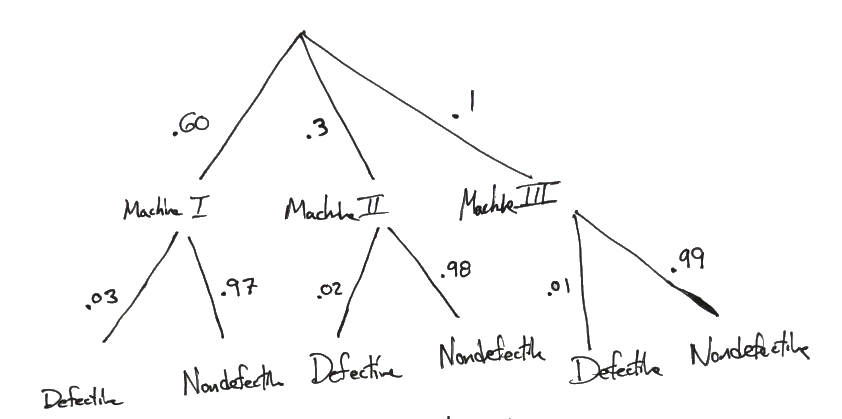
\includegraphics[scale=.3]{images/machines-shells}
  \end{center}

  Let
  \begin{align*}
    D &= [\text{shell is defective}]\\
    M_{1} &= [\text{shell was made by machine I}]\\
    M_{2} &= [\text{shell was made by machine II}]\\
    M_{3} &= [\text{shell was made by machine III}].
  \end{align*}

  We want to find $\P\left[M_{3}\mid D \right]=\P\left[ \text{machine III}\mid \text{defective} \right]$.
  \begin{align}\label{eq:31}
    \P\left[M_{3}\mid D \right]
    &= \frac{\P\left[M_{3}\cap D \right]}{\P\left[D \right]}
  \end{align}
  Now we compute the numerator and denominator separately:

  By the multiplication rule,
  \begin{equation*}
    \P\left[M_{3}\cap D \right] = \P\left[D\mid M_{3} \right] \P\left[M_{3} \right] = (.01)(.1) = .001.
  \end{equation*}
  Next, we compute the denominator. The following figure illustrates the
  sample space, which consists of shells produces by machines I, II and III.
  The grey region represents the event that the randomly selected shell is defective.
  \begin{center}
    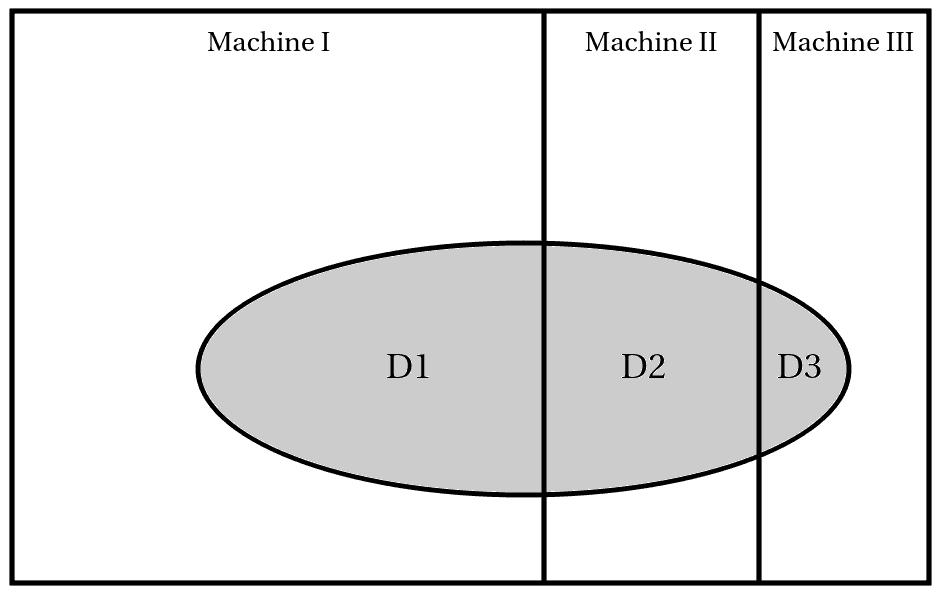
\includegraphics[scale=.3]{images/defective-shells}
  \end{center}
  \begin{align*}
    \P\left[D \right]
    &= \P\left[D1 \right] + \P\left[D2 \right] + \P\left[D3 \right]\\
    &= \P\left[D\cap M_{1} \right]+\P\left[D\cap M_{1} \right]+\P\left[D\cap M_{1} \right]\\
    &= \P\left[D\mid M_{1} \right]\P\left[M_{1} \right] + \P\left[D\mid M_{2} \right]\P\left[M_{2} \right] + \P\left[D\mid M_{3} \right]\P\left[M_{3} \right]\\
    &= (.03)(.6)+(.02)(.3)+(.01)(.1)\\
    &= .025
  \end{align*}
  Hence by \cref{eq:31},
  \begin{equation*}
    \P\left[M_{3}\mid D \right] = \frac{.001}{.025}=.04.
  \end{equation*}
  In other words, $4\%$ of defective rounds are produced by machine III.
  
\end{example}

\begin{example}[Conditional probability]
  Suppose you flip a coin 10 times and get more than $6$ heads. What's the probability that you get less
  than 9 heads?

  \fl{Solution:} Let $X$ be the number of heads. Let $A=\left[ X < 9\right]$, and let
  $B = \left[X > 6\right]$. Then
  \begin{equation*}
    \P\left[B \right] = \frac{{10\choose 7} + {10\choose 8} + {10\choose 9} + {10\choose 10}}{2^{10}}
  \end{equation*}
  Observe that $A\cap B = \left[ X\in \left\{7,8\right\} \right]$. Therefore
  \begin{equation*}
    \P\left[A\cap B \right] = \frac{{10\choose 7}+{10\choose 8}}{2^{10}}
  \end{equation*}
  Therefore
  \begin{equation*}
    \P\left[A\mid B \right] 
    = \frac{\P\left[A\cap B \right]}{\P\left[B \right]} 
    = \frac{{10\choose 7} + {10\choose 8}}{{10\choose 7} + {10\choose 8} + {10\choose 9} + {10\choose 10}} 
    = \frac{15}{16}.
  \end{equation*}
\end{example}


\newpage
\section{2026-02-06 | Week 04 | Lecture 11}

\subsection{Application of the law of total probability: diagnostic tests}
\textit{This based on section 2.4}

\begin{example}[Bayes' Theorem]
  \label{ex:bayes-theorem}
  Prevalance of a disease in a population is $1\%$. A new diagnostic test is advertised as having a false
  positive rate of $.1$ and a false negative rate of $.2$. (In other words, 10\% of positive tests are
  wrong, and 20\% of negative tests are wrong.) Suppose you are selected for a random screening, and you
  test posititve. What's the chance that you have the disease?

  \begin{center}
    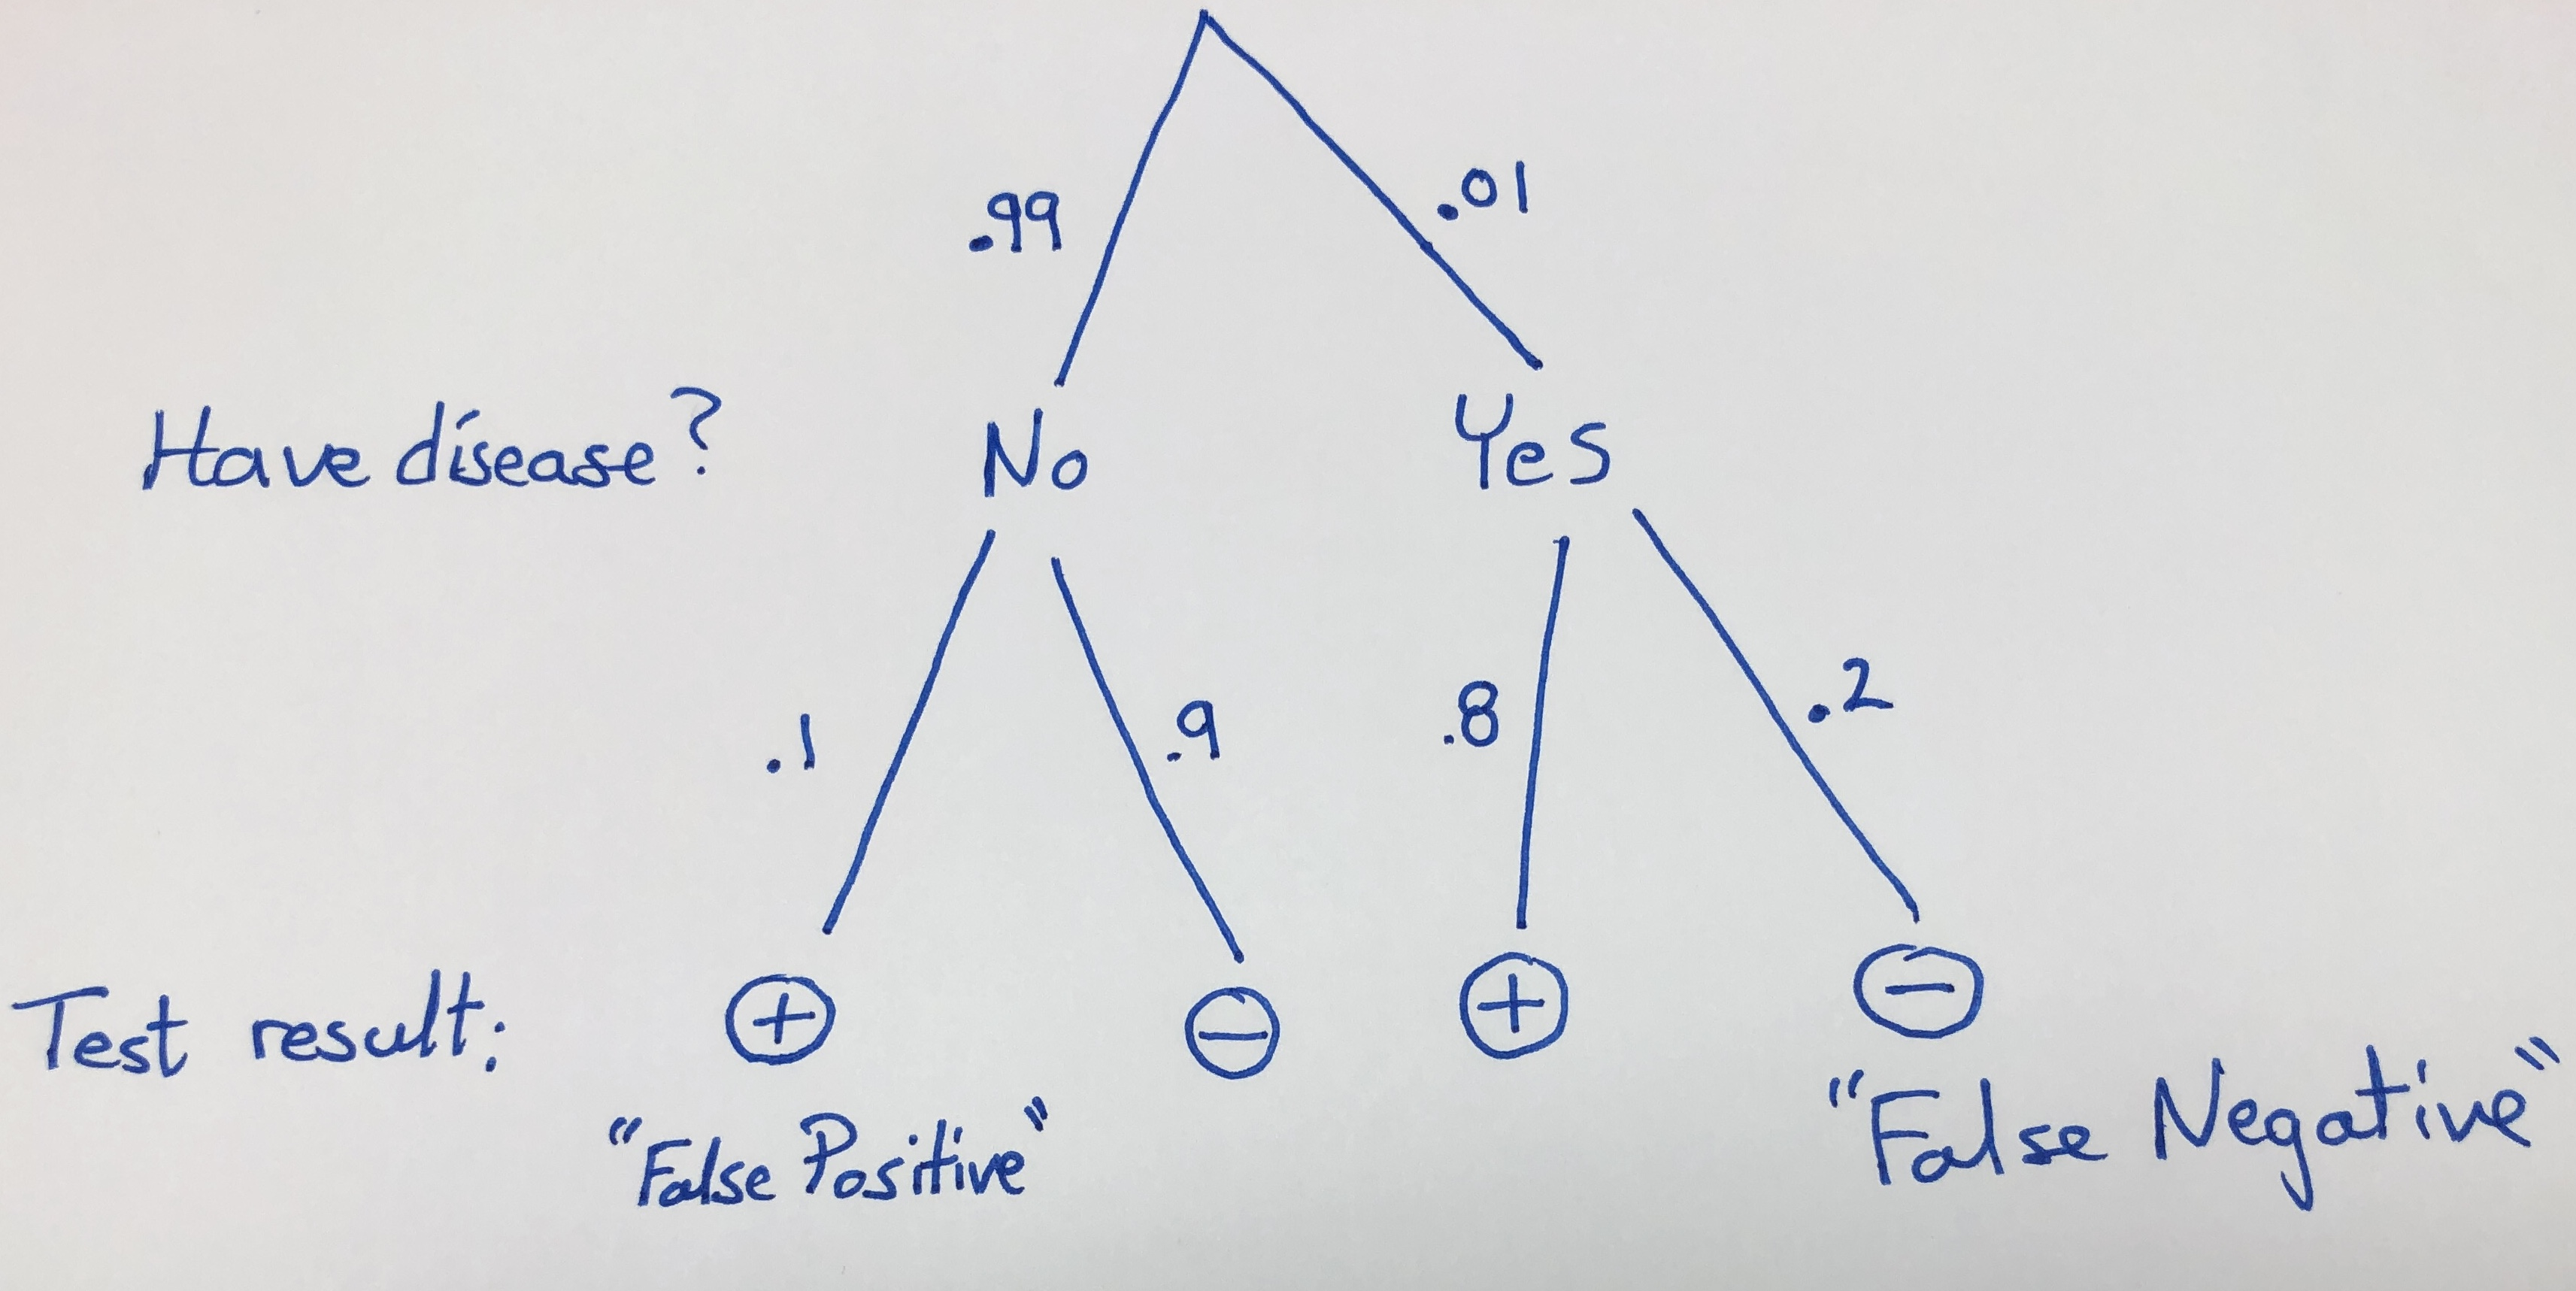
\includegraphics[scale=.08]{images/diagnostic-test}
  \end{center}

  We want $\P\left[ \text{have disease}\mid\text{test positive} \right]$. For brevity, let's let
  \begin{equation*}
    D = \left[ \text{have disease} \right]  \quad \text{and} \quad T^{+} = \left[ \text{test positive} \right].
  \end{equation*}
  In other words, we want
  \begin{equation*}
    \P\left[D\mid T^{+} \right]
  \end{equation*}
  By the definition of conditional probability,
  \begin{align}\label{eq:3}
    \P\left[ D \mid T^{+}\right]
    &= \frac{\P\left[T^{+} \cap D \right]}{\P\left[T^{+} \right]}
  \end{align}
  We will compute the numerator and denominator separately:
  \begin{itemize}
    \item (Numerator) By the multiplication rule for conditional probability ($\P\left[A\cap B
    \right]=\P\left[A|B \right] \P\left[B \right]$), we have
    \begin{equation*}
      \P\left[ T^{+}\cap D \right] = \P\left[T^{+}\mid D \right] \P\left[D \right] = (.8)(.01) = 0.008.
    \end{equation*}
    We've now computed the numerator of \cref{eq:3}.

    \item (Denominator) By the law of total probability,
    \begin{align*}
      \P\left[T^{+} \right] 
      &= \underbrace{\P\left[T^{+}| D \right]\P\left[D \right]}_{=0.008 \text{
        by \cref{eq:4}}}+ \underbrace{\P\left[T^{+}\mid D^{c} \right] \P\left[D^{c} \right]}_{=(.1)(.99) = 0.099}\\
      &= (.8)(.01)+ (.1)(.99)\\
      &= 0.008+ 0.099
    \end{align*}
  \end{itemize}

  Finally, having done the necessary work, we can now plug our results into \cref{eq:3}:
  \begin{equation*}
    \P\left[D\mid T^{+} \right] = \frac{0.008}{0.008 + 0.099} \approx .075
  \end{equation*}
  We conclude that if test positive in a random screening, your probability of actually having the
  disease is about 7.5\%. Is this result surprising?
\end{example}

\subsection{Independence}
\textit{This is based on section 2.5 in the textbook.}

Previously, we saw that $A$ and $B$ have a \textbf{positive relationship} if
\begin{equation*}
  \P\left[B\mid A \right]> \P\left[B \right]
\end{equation*}
and a \textbf{negative relationship} if
\begin{equation*}
  \P\left[B\mid A \right]< \P\left[B \right]
\end{equation*}
What about when $\P\left[B\mid A \right] = \P\left[B \right]?$

\begin{definition}[Independence]
  \label{def:independence}
  Two events $A$ and $B$ are said to be \demph{independent} if $\P\left[A\cap
    B \right] = \P\left[A \right] \P\left[B \right]$. Otherwise, the events
  are said to be \demph{dependent}.
\end{definition}

This definition generalizes in the natural way:

\begin{definition}[Mutual independence]
  \label{def:mutual-independence}
  For any $n \geq 2$, we say that the events $A_{1},\ldots,A_{n}$ are
  \demph{mutually independent} if
  \begin{equation*} 
    \P\left[A_{1}\cap A_{2}\cap\cdots \cap A_{n} \right] = \P\left[A_{1} \right] \P\left[A_{2} \right]\cdots \P\left[A_{n} \right].
  \end{equation*}
\end{definition}


\begin{proposition}
  \label{prop:independence-interpretation}
  If $A,B$ are events with positive probabilities then the following are
  equivalent:
  \begin{enumerate}[label=\rm{(\roman*.)}]
    \item $A$ and $B$ are independent.
    \item \label{item:1} $\P\left[A\mid B \right] = \P\left[A \right]$
    and $\P\left[B\mid A \right] = \P\left[B \right]$ 
  \end{enumerate}
\end{proposition}
\begin{remark}
  \ref{item:1} says that $A$ and $B$ have neither a positive nor negative
  relationship. In words, independence means that the probabilities of each
  event are unaffected by whether or not the other event occurs.
  \cref{prop:independence-interpretation} simply formalizes this idea using
  conditional probabilities.
\end{remark}

\begin{remark}
  A common mistake is to mix up ``independence'' with ``mutually exclusive''.
  Mutually exclusive events are typically \textbf{not} independent. That's because if
  you know that one happened, then you know that the other didn't. That's
  about as far from independence as you can get!
\end{remark}

\newpage
\section{2026-02-11 | Week 05 | Lecture 12}

\subsection{Examples of using independence}
\textit{This is based on chapter 2.5 in the textbook.}

Recall that two events $A$ and $B$ are \textbf{independent} if
$\P\left[A\cap B \right]=\P\left[A \right]\P\left[B \right]$. This means that knowledge of one event gives no information about the other.

% \begin{example}[Example 2.34 in textbook]
%   It is known that $30\%$ of a company's washing machines require service in
%   the first five years, wheras only $10\%$ of their dryers need such service.
%   If someone purchases a washer and dryer, what is the probability that both
%   will need service in the first five years?

%   \fl{Solution:} Let $A$ be the event that the washer will need service, and
%   let $B$ be the event that the dryer will need service. Then
%   \begin{equation*}
%     \P\left[A\cap B \right] = \P\left[A \right] \P\left[B \right] = (.3)(.1)=.03.
%   \end{equation*}
% \end{example}

\begin{example}
  The proportions of blood types in the US are
  \begin{center}
    A: 40\% \quad  B: 11\% \quad AB: 4\% \quad O: 45\%
  \end{center}
  \begin{enumerate}[(a)]
    \item What is the probability that two randomly-selected people are both
    $O$.
    
    \fl{Solution:} Assuming that the two blood types are independent, we have
    \begin{align*}
      \P\left[ \text{person 1 has O blood} \cap \text{person 2 has O blood}
      \right] 
      &= \P\left[\text{person 1 has O blood} \right]
        \P\left[\text{person 2 has O blood} \right] \\
      &= (.45)(.45) \\
      &= 0.2025.
    \end{align*}
    \item What is the probability that two randomly-selected people have
    matching blood types?
    
    \fl{Solution:} Let $M$ be the event that the people have matching blood
    type, and let $M_{X}$ be the event that both people have type $X$
    blood, for $X\in \left\{A,B,AB,O\right\}$.

    \begin{align*}
      \P\left[M \right] 
      &= \P\left[M_{A}\cup M_{B}\cup M_{AB}\cup M_{O} \right]\\
      &= \P\left[M_{A} \right] + \P\left[M_{B} \right]+ \P\left[M_{AB} \right] + \P\left[M_{O} \right],
    \end{align*}
    where the last equality followed from the fact that the events
    $M_{A},M_{B},M_{AB},M_{O}$ are pairwise disjoint.
    
    We already computed $\P\left[M_{O} \right]= (.45)(.45) = .2025$. By similar calculations,
    we get
    \begin{equation*}
      \P\left[M \right] = (.40)(.40)+(.11)(.11)+ (.04)(.04) + (.45)(.45) = .3762.
    \end{equation*}
  \end{enumerate}
\end{example}

\subsection{Dicrete Random Variables}
\textit{Based on sections 3.1 and 3.2 of the textbook}

We often associate numbers with outcomes of an experiment.

\begin{definition}[Random variables]
  \label{def:random-variables}
  Let $S$ be a sample space of an experiment. A \demph{random variable} is any
  rule that associates a number with each outcome in $S$. In other words, it
  is a function whose domain is $S$ and whose range is $\R$.
\end{definition}

The value of a random variable is thought of as varying depending on the
outcome of the experiment. Random variables are usually denoted with capital
letters, like $X,Y,Z$.

\begin{example}
  \label{ex:sum-2d4}
  Roll a 4-sided dice twice (this is the \textbf{experiment}). There are 16
  possible \textbf{outcomes}. The \textbf{sample space} is
  \begin{equation*}
    S = \left\{(x,y): x,y\in \left\{1,2,3,4\right\} \right\}.
  \end{equation*}
  Let $X$ be the sum of the two rolls. We can represent $X$ by the following
  table:
  \begin{equation*}
    \begin{array}{c@{\quad}c|cccc} & \multicolumn{5}{c}{\text{Dice 2}} \\ & &
      1 & 2 & 3 & 4 \\ \cline{2-6}  & 1 & 2 & 3 & 4 & 5 \\ \text{Dice 1} & 2 & 3 & 4 & 5 & 6 \\ & 3 & 4 & 5 & 6 & 7 \\ & 4 & 5 & 6 & 7 & 8 \end{array}
  \end{equation*}
\end{example}

\begin{definition}[Discrete random variable]
  We say that a random variable $X$ is a \demph{discrete random variable} if
  it can assume only a finite or countably infinite number of distinct values.
\end{definition}


\begin{definition}[Probability mass function (pmf)]
  \label{def:probability-mass-function-pmf}
  Let $X$ be a discrete random variable. The \demph{probability mass function}
  (or \demph{pmf}) of $X$ is the function
  \begin{equation*}
    p(x) = \P\left[X=x \right],
  \end{equation*}
  defined for every $x\in \R$.
\end{definition}

\begin{example}
  The pmf of $X$ in \cref{ex:sum-2d4} is
  \begin{equation*}
    p(2) = 1/16 \quad p(3) = 2/16, \quad p(4) = 3/16, \quad p(5) = 4/16, \quad p(6) = 3/16, \quad p(7)=2/16, \quad p(8) = 1/16
  \end{equation*}
  and $p(x)=0$ for all other $x\in \R$. It is often useful to write these as a
  table:
  \begin{center}
    \begin{tabular}{l|l}
      $x$ & $\P[X=x]$ \\ \hline
      2   & $1/16$     \\
      3   & $2/16$     \\
      4   & $3/16$     \\
      5   & $4/16$    \\
      6   & $3/16$    \\
      7   & $2/16$    \\
      8   & $1/16$    
    \end{tabular}
  \end{center}
\end{example}

\begin{definition}
  For a discrete random variable $X$, the \demph{expected value} of $X$,
  denoted $\E\left[X \right]$, is
  \begin{equation*}
    \E\left[X \right] = \sum_{x}x \P\left[X=x \right] 
  \end{equation*}
  where the sum ranges over all distinct values that $X$ can take.
\end{definition}

\begin{remark}
  $\E\left[X \right]$ is the long-run average of $X$, if we were to repeat the
  experiment many times.
\end{remark}

\begin{example}
  Let $X$ be the random variable in \cref{ex:sum-2d4}. Then
  \begin{align*}
    \E\left[X \right] 
    &= \sum_{x}x \P\left[X=x \right]\\
    &=2 \left( \frac{1}{16} \right) +
      3 \left( \frac{2}{16} \right) +
      4 \left( \frac{3}{16} \right) +  
      5 \left( \frac{4}{16} \right) +  
      6 \left( \frac{3}{16} \right) +  
      7 \left( \frac{2}{16} \right) +  
      8 \left( \frac{1}{16} \right)\\
    &= \frac{80}{16}\\
    &=5.
  \end{align*}
  Therefore, the sum of two 4-sided dice rolls is, on average, 5.
\end{example}

\begin{definition}[Cumulative distribution function (cdf)]
  \label{def:cumulative-distribution-function-cdf}
  Let $X$ be any random variable. The \demph{cumulative distribution function}
  (or \demph{cdf}) of $X$ is the function
  \begin{equation*}
    F(x) = \P\left[X \leq x\right],
  \end{equation*}
  defined for all $x\in \R$.
\end{definition}

\begin{example}
  For the random variable in \cref{ex:sum-2d4}, the cdf is given by the
  following table
  \begin{center}
    \begin{tabular}{l|l}
      $x$ & $F(x) = \P[X \leq x]$ \\ \hline
      2   & $1/16$     \\
      3   & $3/16$     \\
      4   & $6/16$     \\
      5   & $10/16$    \\
      6   & $13/16$    \\
      7   & $15/16$    \\
      8   & $1$    
    \end{tabular}
  \end{center}

  Here is a plot of $F(x)$. It is the step function shown in blue:

  \begin{center}
    \begin{tikzpicture}[x=1.2cm,y=6cm,scale=.8]

      % axes
      \draw[->] (0,0) -- (10,0) node[right] {$x$};
      \draw[->] (0,0) -- (0,1.05) node[above] {$$};

      % x-axis ticks
      \foreach \x in {1,2,3,4,5,6,7,8,9}
      {
        \draw (\x,.01) -- (\x,-0.01);
        \node[below] at (\x,0) {\small $\x$};
      }

      % y-axis ticks
      \foreach \y/\lab in {
        0.0625/{1/16},
        0.1875/{3/16},
        0.3750/{6/16},
        0.6250/{10/16},
        0.8125/{13/16},
        0.9375/{15/16},
        1/{1}
      }
      {
        \draw (.04,\y) -- (-.04,\y);
        \node[left] at (0,\y) {\small $\lab$};
      }

      % horizontal pieces
      \draw[thick,blue,<-] (0,0) -- (2,0);
      \draw[thick,blue] (2,0.0625) -- (3,0.0625);
      \draw[thick,blue] (3,0.1875) -- (4,0.1875);
      \draw[thick,blue] (4,0.3750) -- (5,0.3750);
      \draw[thick,blue] (5,0.6250) -- (6,0.6250);
      \draw[thick,blue] (6,0.8125) -- (7,0.8125);
      \draw[thick,blue] (7,0.9375) -- (8,0.9375);
      \draw[thick,blue,->] (8,1.0000) -- (10,1.0000);

      % open circles
      \foreach \x/\y in {
        2/0, 3/0.0625, 4/0.1875, 5/0.3750, 6/0.6250, 7/0.8125, 8/0.9375}
      \draw[blue,fill=white] (\x,\y) circle (1.6pt);

      % closed circles
      \foreach \x/\y in {
        2/0.0625, 3/0.1875, 4/0.3750, 5/0.6250, 6/0.8125, 7/0.9375, 8/1.0000}
      \fill[blue] (\x,\y) circle (1.6pt);

    \end{tikzpicture}
  \end{center}

  For dicrete random variables, the graph of a cdf will always look similar to
  the above: it will be an increasing step function with open circles on the
  right endpoints and filled-in circles on the left endpoints.
\end{example}


\newpage
\section{2026-02-13 | Week 05 | Lecture 13}

\subsection{Exam review problems}
We went over some example problems:
\begin{itemize}
  \item The solution to problem 1 on homework 2. The key idea involves
  correctly filling out the venn diagram as shown:
  \begin{center}
    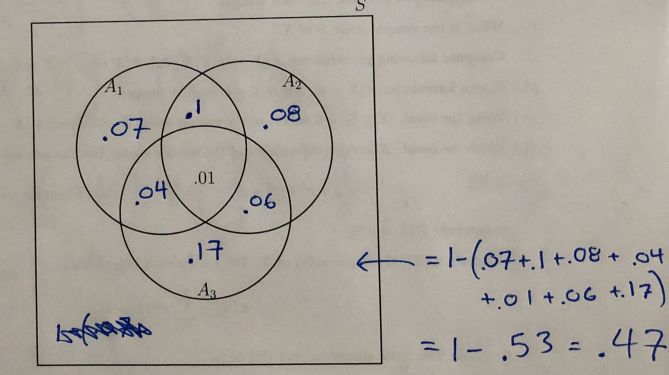
\includegraphics[scale=.3]{images/hw2-solution}
  \end{center}
  \item The solution to problem 14 on homework 4. 
  \item An example about computing probabilities invovling the phrase ``at
  least'' (shown below).
\end{itemize}

\begin{example}
  Suppose we roll a 6-sided dice three times. What's the probability that we
  get at least one 6?

  \Fl{Solution:} The key idea is the following
  \begin{equation*}
    \P\left[\text{at least one six is rolled} \right] = 1 - \P\left[\text{no
        sixes are rolled} \right]
  \end{equation*}

  To put this idea into practice, let
  $A_{1}= \left[ \text{the first dice roll is a 6} \right]$,
  $A_{2} = \left[ \text{the second dice roll is a 6} \right]$, and
  $A_{3}= \left[ \text{the third dice roll is a 6} \right]$. Clearly,
  $A_{1},A_{2},A_{3}$ are independent because the dice rolls don't influence
  each other. Then
  \begin{align*}
    \P\left[ \text{at least one six is rolled}\right] 
    &= \P\left[A_{1}\cup A_{2}\cup A_{3} \right]\\
    &= 1- \P\left[A_{1}^{c}\cap A_{2}^{c}\cap A_{3}^{c} \right] && \text{by de
                                                                   Morgan's law}\\
    &= 1 - \P\left[A_{1}^{c} \right] \P\left[A_{2}^{c} \right]
      \P\left[A_{3}^{c} \right] &&\text{by independence}\\
    &= 1 - \left( \frac{5}{6} \right) \left( \frac{5}{6} \right) \left( \frac{5}{6} \right)\\ 
    &= 1- \left( \frac{5}{6} \right)^{3}.
  \end{align*}
  
\end{example}

\newpage


\section{2026-02-23 | Week 07 | Lecture 14}
\textit{This lecture is based on chapter 3.3 in the textbook.}
\subsection{Expectation}
Recall that the \demph{expected value} of a discrete random variable is
\begin{equation*}
  \mu = \E\left[X \right] = \sum_{x} x\cdot p(x) 
\end{equation*}
where the $x$ in the summation runs over all possible values of $X$. 

In words, the expected value is the \textit{long-run average}, meaning that if
you repeated an experiment many times (independently), the long-run average
would converge to $\E\left[X \right]$.

\begin{remark}[Notation]
  We sometimes use the notation $\mu$ or $\mu_{X}$ for $\E\left[X \right]$.
\end{remark}

The following is a simple but important fact:

\begin{proposition}[Linearity of Expectation]
  \label{prop:linearity-of-expectation}
  Let $a,b$ be numbers and $X$ and $Y$ be a random variables. Then
  \begin{equation*}
    \E\left[aX+b \right] = a \E\left[X \right] +b
  \end{equation*}
  and
  \begin{equation*}
    \E\left[aX+bY \right] = a\E\left[X \right]+ b\E\left[Y \right].
  \end{equation*}
\end{proposition}
We saw this earlier, when we looked at the expected value of playing the
lottery once $(-\$1)$ and of playing $10$ times $(-\$10)$, etc.

\begin{theorem}[Expectation of a function of $X$] 
  \label{thm:LOTUS-discrete-case}
  Let $X$ be a discrete random variable with pmf $p(x)$. Let $h:\R \to \R$ be any function. Then
  \begin{equation*}
    \E\left[h(X) \right] = \sum_{x} h(x)p(x) 
  \end{equation*}
  provided that the sum on the right hand side is absolutely convergent. As usual, the summation runs
  over all possible values of $X$.
\end{theorem}

\begin{example}
  Suppose $Y$ is a discrete random variable with pmf
  \begin{gather*}
    p(-2) = \P\left[Y = -2 \right] = 0.1 \\ p(-1) = \P\left[Y=-1 \right] = 0.3 \\ p(1) = \P\left[Y=1 \right] =0.4 \\  p(2) = \P\left[Y=2 \right] = 0.2
  \end{gather*}
  and such that $\P\left[Y=y \right] = 0$ if $y\notin \left\{-2,-1,1,2\right\}$
  % 
  Find the following quantities:
  \begin{enumerate}[(a)]
    \item $\E\left[Y \right]$
    \item $\E\left[3Y+7 \right]$
    \item $\E\left[Y^{3}+2Y \right]$
    \item $\E\left[e^{X} \right]$
  \end{enumerate}

  \textit{Solution to (a):}
  \begin{align*}
    \E\left[Y \right] 
    &= -2(0.1)+(-1)(0.3)+(1)(0.4)+(2)(0.2)\\
    &= -.2 -.3 +.4 + .4\\
    &= .3
  \end{align*}

  \textit{Solution to (b):}
  \begin{align*}
    \E\left[3Y+7 \right] 
    &= 3 \E\left[Y \right]+7
    &&\text{by \cref{prop:linearity-of-expectation} }\\
    &= 3(0.3)+7
    &&\text{by our answer to part (a). }\\
    &= 7.9.
  \end{align*}

  \textit{Solution to (c):} Here we will apply  \cref{thm:LOTUS-discrete-case} with $h(x)=x^{3}+2x$:
  \begin{align*}
    \E\left[Y^{3}+2Y \right] 
    &= \sum_{y\in \left\{-2,-1,1,2\right\}} h(x)p(x)\\
    &= h(-2)p(-2)+h(-1)p(-1)+h(1)p(1)+h(2)p(2)\\
    &= (-12)(0.1)+(-3)(0.3)+(3)(0.4)+(12)(0.2)\\
    &= 1.5.
  \end{align*}

  \textit{Solution to (d):} Here we will apply \cref{thm:LOTUS-discrete-case} with $h(x) =
  e^{x}$:
  \begin{align*}
    \E\left[e^{Y} \right] 
    &= \sum_{y\in \left\{-2,-1,1,2\right\}} h(y)p(y)\\
    &= \sum_{y\in \left\{-2,-1,1,2\right\}} e^{y}p(y)\\
    &= e^{-2}p(-2)+ e^{-1}p(-1)+e^{1}p(1)+e^{2}p(2)\\
    &= e^{-2}\cdot0.1+ e^{-1}\cdot0.3+e^{1}\cdot0.4+e^{2}\cdot0.2\\
    &\approx 2.689.
  \end{align*}
\end{example}

% We'll be interested in some
% special cases
% \begin{itemize}
%   \item $h(x) = x^{2}$
%   \item $h(x) = (x-\mu)^{2}$, where $\mu= \E\left[X \right]$.
%   \item $h(x) = e^{tX}$, where $t$ is any fixed real number.
% \end{itemize}

\subsection{Variance}
\begin{definition}[Variance]
  \label{def:variance}
  The \demph{variance} of a random variable $X$ is
  \begin{equation*}
    \text{Var}(X) := \E\left[(X-\mu)^{2} \right]
  \end{equation*}
  where $\mu= \E\left[X \right]$. (Note: variance is often denoted by $\sigma^{2}$)
\end{definition}

Variance is a measure of how likely the value of a random variable is to be far from its expected value.
In an ideal world, we would measure this by
\begin{equation*}
  \E\left[\left| X-\mu \right| \right] = (\text{expected distance of $X$ from its mean})
\end{equation*}
But unfortunately, the absolute value function is mathematically difficult to work with, so instead we
use
\begin{equation*}
  \E\left[(X-\mu)^{2} \right] = \text{Var}(X)
\end{equation*}
which is mathematically easer to work with because it doesn't have an absolute value.

\begin{example}
  Let $X$ and $Y$ be random variables defined as follows:
  \begin{equation*}
    X = \left\{ \begin{array}{l@{\quad:\quad}l} +1 & \text{with probability
        }\frac{1}{2} \\ -1& \text{with probability }\frac{1}{2} \end{array}\right.
    \quad \text{and} \quad
    Y = \left\{ \begin{array}{l@{\quad:\quad}l} +1000 & \text{with probability
        }\frac{1}{2} \\ -1000& \text{with probability }\frac{1}{2} \end{array}\right.
  \end{equation*}
  In both cases, $\E\left[X \right]=0$ and $\E\left[Y \right] = 0$. But
  despite having the same expected value, these are very different random
  variables: the value of $Y$ deviates from its mean much more than $X$ does.
  Indeed, direct computation (shown below) shows the variance of $Y$ to be
  much larger than the variance of $X$:
  \begin{align*}
    \Var(X) 
    &= \E\left[(X- \mu)^{2} \right] \\
    &= \E\left[X^{2} \right] &&\text{ since $\mu= \E\left[X \right]=0$ }\\
    &= (1)^{2}(.5)+(-1)^{2}(.5) &&\text{ by \cref{thm:LOTUS-discrete-case} }\\
    &= 1.
  \end{align*}
  On the other hand,
  \begin{align*}
    \Var(Y) 
    &= \E\left[(Y- \mu)^{2} \right] \\
    &= \E\left[Y^{2} \right] &&\text{ since $\mu= \E\left[Y \right]=0$ }\\
    &= (1000)^{2}(.5)+(-1000)^{2}(.5) &&\text{ by \cref{thm:LOTUS-discrete-case} }\\
    &= 1000000.
  \end{align*}
\end{example}

\newpage
\section{2026-02-25 | Week 07 | Lecture 15}


\subsection{Properties of Variance}
Recall that the \demph{variance} of a random variable $X$ is
\begin{equation*}
  \Var(X) = \E\left[(X-\mu)^{2} \right]
\end{equation*}
where $\mu= \E\left[X \right]$.

For a discrete random variable $X$, this expectation can be written as
\begin{equation*}
  \Var(X) = \sum_{x}(x-\mu)^{2}\P\left[X=x \right]
\end{equation*}
by \cref{thm:LOTUS-discrete-case}.

The positive square root of the variance is called the \demph{standard deviation}.

There is a shortcut for computing variance, given in the next theorem.
\begin{theorem}[Variance shortcut formula]
  \label{thm:variance-shortcut-formula}
  Let $X$ be a random variable with $\E\left[X^{2} \right]<\infty$. Then
  \begin{align*}
    \Var(X) 
    &= \E\left[X^{2} \right] - \left( \E\left[X \right] \right)^{2}
  \end{align*}
\end{theorem}
The condition $\E\left[X^{2} \right]<\infty$ in
\cref{thm:variance-shortcut-formula} is there to exclude the possibility that
the right hand side of the formula be the undefined form $\infty-\infty$.

% \begin{example}
%   Suppose
%   \begin{equation*}
%     U =  \left\{ \begin{array}{l@{\quad:\quad}l} 2 & \text{with probability }\alpha\\ 3& \text{with
%           probability }1-\alpha \end{array}\right.
%   \end{equation*}
%   What is $\E\left[U \right]$ and $\Var(U)$?

%   \textit{Solution:} First, we will compute the expectation:
%   \begin{align}\label{eq:8}
%     \E\left[U \right] 
%     &= 2\alpha+3(1-\alpha) \nonumber\\
%     &= 3-\alpha
%   \end{align}

%   Next, we will compute $\Var(U)$. We will use the formula  \cref{eq:7}. In particular we wil need
%   $\E\left[U^{2} \right]$, so let's compute that:
%   \begin{align}\label{eq:9}
%     \E\left[U^{2} \right] 
%     &=2^{2}\alpha+3^{2}(1-\alpha) &&\text{by \cref{thm:expectation-of-function-of-X} }\nonumber\\
%     &=4\alpha+9(1-\alpha)\nonumber\\
%     &=9-5\alpha
%   \end{align}
%   We can now plug the values from \cref{eq:9,eq:8} into \cref{eq:7} to get
%   \begin{align*}
%     \Var(U) 
%     &= \E\left[U^{2} \right] - \left( \E\left[U \right] \right)^{2}\\
%     &= 9-5\alpha - (3-\alpha)^{2}
%   \end{align*}
%   For example, if $\alpha=\frac{1}{2}$, then we get
%   $\E\left[U \right] = 3-\frac{1}{2} = 2.5$
%   and
%   \begin{equation*}
%     \Var(U) = 9-\frac{5}{2}- \frac{25}{4} = \frac{1}{4}
%   \end{equation*}
%   Now, someone asked ``how do we interpret this $1/4$?'' The short answer is, it's complicated. There
%   isn't a nice interpretation that works for every random variable, so often the best we can do is
%   understand this as some measure of how much our random variable tends to deviate from its mean. In this
%   case, the $1/4$ is pretty small, so the random variable doesn't seem to deviate all that much from its
%   mean.
% \end{example}


While variance does give us some information, it's only a single number and so the amount of information
it gives us about the random variable is actually very limited, and it is impossible to interpret it
precisely without additional information about the random variable. This is illustrated in the following
example.

\begin{example}
  Let $M = 1,000,000$. And let
  \begin{equation*}
    X = \left\{ \begin{array}{l@{\quad:\quad}l} 0 & \text{with probability } .99  \\ 10M &
        \text{with probability }.01 \end{array}\right.
  \end{equation*}
  The random variable $X$ is like winning the lottery.

  On the other hand,  let
  \begin{equation*}
    Y = \left\{ \begin{array}{l@{\quad:\quad}l} -10 & \text{with probability }\frac{1}{2}\\ 10 & \text{with probability }\frac{1}{2} \end{array}\right.
  \end{equation*}

  In the case of $X$, we have
  \begin{align*}
    \Var(X) 
    &= \E\left[X^{2} \right] - \left( \E\left[X \right] \right)^{2}\\
    &= \left[(10M)^{2}(0.01)+ 0^{2}(0.99)\right] - \left[10M(0.01)+ 0(0.99)\right]^{2}\\
    &= M^{2} - \frac{M^{2}}{100}\\
    &= \frac{99}{100}M^{2}
  \end{align*}
  This is a HUGE variance, because $M=10,000,000$. But for the most part, intuitvely, few people would
  say that this r.v. ``varies'' all that much. After all, it's almost always $0$.


  On the other hand, what if we compute the variance of $Y$? In this, we have $\E\left[Y
  \right]=-10\frac{1}{2}+10\frac{1}{2}=0$, so
  \begin{align*}
    \Var(Y) 
    &= \E\left[Y^{2} \right]-0\\
    &= (-10)^{2}\frac{1}{2} + (10)^{2}\frac{1}{2}\\
    &= 100
  \end{align*}
  In this case, the variance is pretty big---not huge, but pretty big. Yet the random variable $Y$
  doesn't really seem to ``vary'' all that much: after all, we know it is always either 10 more than the
  mean (which is zero), or 10 less than the mean.
\end{example}

Hopefully this example doesn't give you the impression that variance is useless. It's actually a really
important measure. The issue is just that random variables can ``vary'' in lots of different ways that
can be hard to summarize as a single value.

Variance has several properties that are often useful, described in the next
theorem.

\begin{theorem}[Properties of Variance]
  \label{thm:variance-properties}
  Let $X$ be a random variable. Then:
  \begin{itemize}
    \item For any scalars $a,b$,
    \begin{equation}\label{eq:5}
      \Var(aX+b) = a^{2}\Var(X).
    \end{equation}
    \item If $X$ and $Y$ are independent random variables then
    \begin{equation}\label{eq:7}
      \Var(aX+bY+c) = a^{2}\Var(X)+b^{2}\Var(Y).
    \end{equation}
  \end{itemize}
\end{theorem}
\fl{Implications of \cref{thm:variance-properties}:}
\begin{itemize}
  \item Taking $b=0$ in \cref{eq:5} gives
  \begin{equation}\label{eq:variance-squre-scaling}
    \Var(aX) = a^{2}\Var(X).
  \end{equation}
  \begin{proof}[Here is a direct proof of \cref{eq:variance-squre-scaling}:]
    \begin{align*}
      \Var(aX)
      &= \E\left[\left( aX- \E\left[aX \right] \right)^{2}  \right]
      &&\text{by \cref{def:variance}}\\
      &= E\left[  \left( aX- a\E\left[X \right] \right)^{2}  \right]
      &&\text{by \cref{prop:linearity-of-expectation}}\\
      &= \E\left[a^{2}\left(X- \E\left[X \right]  \right)  \right]\\
      &= a^{2} \E\left[ X- \E\left[X \right]   \right] &&\text{by \cref{prop:linearity-of-expectation}}\\
      &= a^{2}\Var(X) &&\text{by \cref{def:variance} }
    \end{align*}
  \end{proof}
  \item Taking $a=1$ in \cref{eq:5} gives
  \begin{equation*}
    \Var(X+b) = \Var(X)
  \end{equation*}
  which says that adding a nonrandom quantity to a random variable doesn't
  change its variance.
  \item Taking $a=b=1$ and $c=0$ in \cref{eq:7} implies that
  \begin{equation}\label{eq:additivity-of-variance}
    \Var(X+ Y) = \Var(X) + \Var(Y).
  \end{equation}
  This says that for independent random variables, variance is additive.

  (Of course, we always have
  $\E\left[X+Y \right] = \E\left[X \right]+ \E\left[Y \right]$, even if $X$
  and $Y$ are not independent. This is called \demph{linearity of
    expectation}. But for variance, we need $X$ and $Y$ to be independent to
  do something similar.)
\end{itemize}




\subsection{Binomial random variable}

% \begin{example}[Bernoulli random variable]
%   Any random varible whose only values are 0 or 1. For any fixed value $0<\alpha<1$, we say that $X$ \demph{is a
%     Bernoulli random variable with success parameter $\sigma$} if
%   \begin{equation*}
%     X = \left\{ \begin{array}{l@{\quad}l} 1 & \text{with probability } \alpha\\0  & \text{with
%           probability } 1-\alpha \end{array}\right.
%   \end{equation*}
%   In this case, we write $X\sim \text{Bern}(\alpha)$. 
%   The pmf of $X$ is the function taking the following values:
%   \begin{equation*}
%     p(1) = \alpha,
%     \quad  p(0) = 1-\alpha,
%     \quad \text{and} \quad p(x)=0 \text{ for all other values of }x
%   \end{equation*}
  
%   A Bernoulli random variable is nothing other than a coin flip (with a coin that lands `head' with
%   probability $\alpha$.)
% \end{example}

Next we introduce an important type of random variable, called the
``binomial'' random variable. The motivation is the following idea: if you
flip a coin $n$ times, and let $p\in (0,1)$ be the probability of `heads'
on any given coin flip. We can define a random variable
$X=\text{(\# of heads in $n$ flips)}$.

The probability that you get exactly $k$ heads in $n$ flips is given by the formula:
\begin{equation}\label{eq:32}
  {n\choose k} p^{k}(1-p)^{n-k}.
\end{equation}
This is the probability that $X=k$. To see where \cref{eq:32} comes from, work
out an example, say $n=5$ and $k=3$, and the general idea will become clear.

The precise definition of a binomial random variable is as follows:

\begin{definition}[Binomial random variable]
  \label{def:binomial-random-variable}
  A random variable is said to be a \demph{Binomial random variable} with $n$
  trials and success probability $p$ if
  \begin{equation*}
    \P\left[X=k\right] = {n\choose k} p^{k}(1-p)^{n-k}
  \end{equation*}
  for every $k\in \left\{0,1,\ldots,n\right\}$. In this case, we write
  $X\sim \text{Bin}(n,p)$.
\end{definition}

\begin{remark}[Useful characterization of binomial random variables]
  \label{rmk:useful-characterization-binomial-random-variables}
  If $X$ is a Binomial random variable with $n$
  trials and success probability $p$, then we can write
  \begin{equation*}
    X = \xi_{1}+\ldots+\xi_{n}
  \end{equation*}
  where
  \begin{equation*}
    \xi_{i} = \left\{ \begin{array}{l@{\quad:\quad}l} 1 & \text{with probability
        }p\\0 & \text{with probability }1-p \end{array}\right..
  \end{equation*}
  In words $\xi_{i}$ is either one or zero depending on whether the
  $i^{\rm th}$ coin flip was `heads' or not. Hence, the sum
  $\xi_{1}+\ldots+\xi_{n}$ counts the number of heads in $n$ coin flips.
\end{remark}

\begin{example}
  Suppose we wish to compute $\E\left[X \right]$, when $X$ is binomial with
  $n$ trials and success parameter $p$.

  To do this computation, we'll use the idea of
  \cref{rmk:useful-characterization-binomial-random-variables}:
  \begin{align*}
    \E\left[X \right] 
    &= \E\left[\xi_{1}+\ldots+\xi_{n} \right]\\ 
    &= \E\left[\xi_{1} \right]+\ldots+ \E\left[\xi_{n} \right] &&\text{by \cref{prop:linearity-of-expectation}}.
  \end{align*}
  Observe that $\E\left[\xi_{i} \right]=1\cdotp+0\cdot(1-p)=p$ for all $i\in
  \left\{1,\ldots,n\right\}$, and hence
  \begin{equation*}
    \E\left[X \right]= n p.
  \end{equation*}
\end{example}
\newpage
\section{2026-02-27 | Week 07 | Lecture 16}

\subsection{Application of the Law of Total Probability: The probability of winning at craps}

Recall the rules of craps:
\begin{enumerate} 
  \item You roll two dice and add them up.
  \begin{itemize}
    \item If the sum is $2,3$, or $12$, you lose (``craps'')
    \item If you roll $7$ or $11$, then you win  (``natural'')
    \item Otherwise you establish ``point'', which is whatever number you got.
  \end{itemize}
  \item If you established point, then you must keep rolling until one of two events occurs:
  \begin{itemize}
    \item You roll a 7: you lose
    \item You roll your ``point'' number: you win.
  \end{itemize}
\end{enumerate}

Let's introduce some useful notation:
Let
\begin{equation*}
  W= \left[ \text{You win} \right],
\end{equation*}
and for each $k=2,3,4,\ldots,12$, define
\begin{equation*}
  F_{k}= \left[ \text{Your first roll is }k \right].
\end{equation*}
\Fl{Question:} What is $\P\left[W \right]$?

\fl{Solution:} By the \textit{Law of Total Probability}, we have
\begin{equation}\label{eq:6}
  \P\left[W  \right] =  \sum_{k=2}^{12} \P\left[W\mid F_{k}\right]\times \P\left[F_{k} \right] 
\end{equation}
In words,
\begin{equation*}
  \P\left[W\mid F_{k}\right] = \text{ probability of winning, given you rolled $n$ on the first roll}
\end{equation*}

\begin{table}[htbp]
  \centering
  \begin{tabular}{l|l|l}
    \textit{\textbf{$k$}} & \textbf{$P[W\mid F_i]$} & \textbf{$\P[F_k]$} \\ \hline
    2                     & 0                       & 1/36               \\
    3                     & 0                       & 2/36               \\
    4                     & 1/3                     & 3/36               \\
    5                     & 4/10                    & 4/36               \\
    6                     & 5/11                    & 5/36               \\
    7                     & 1                       & 6/36               \\
    8                     & 5/11                    & 5/36               \\
    9                     & 4/10                    & 4/36               \\
    10                    & 1/3                     & 3/36               \\
    11                    & 1                       & 2/36               \\
    12                    & 0                       & 1/36              
  \end{tabular}
\end{table}
How do we get, say, $\P\left[W \mid F_{4} \right]$?

\textbf{(Method 1: The long way)} Let's enumerate the ways we can win:
\begin{align*}
  &4 &&\text{win on the first roll after establishing point}\\ 
  &*4 &&\text{win on second roll}\\
  &**4 &&\text{win on third roll }\\
  &***4 &&\text{etc }\\
  &****4\\
  &\cdots
\end{align*}
where $*$ denotes any roll other than a 4 or a 7.

These have probabitilies
\begin{align*}
  &\P\left[4\right] = \frac{3}{36}\\ 
  &\P\left[*4\right] = \frac{27}{36} \frac{3}{36}\\
  &\P\left[**4\right] = \left( \frac{27}{36} \right)^{2} \frac{3}{36} \\
  &\P\left[***4\right]= \left( \frac{27}{36} \right)^{3} \frac{3}{36} \\\\
  &\P\left[****4\right] = \left( \frac{27}{36} \right)^{4} \frac{3}{36} \\\\
  &\cdots
\end{align*}
So
\begin{align*}
  \P\left[W\mid F_{4} \right] 
  &= \frac{3}{36}+ \frac{27}{36}\frac{3}{36}+ \left( \frac{27}{36} \right)^{2} \frac{3}{36} \\
  &= \frac{3}{36} \left( 1 + \frac{27}{36} + \left( \frac{27}{36} \right)^{2}+\ldots  \right) \\
  &= \frac{3}{36}\cdot \frac{1}{1-\frac{27}{36}} \\
  &= \frac{3}{9} \\
  &= \frac{1}{3}.
\end{align*}

\textbf{(Method 2: The short way)}. Given $F_{4}$, you know you're gonna keep rolling until you get a 4 or
a 7, which is eventually going to happen. And whether you win or lose is determined by what you roll on
that last roll. Your probability of winning is the probability of rolling a 4 on your last roll, given
that your last roll is a 4 or a 7. Thus,

\begin{align*}
  \P\left[W\mid F_{4} \right] 
  &= \P\left[ \text{roll 4} \mid \text{roll 4 or 7} \right] \\
  &= \frac{\P\left[ \text{(roll 4) and (roll 4 or 7)} \right]}{\P\left[ \text{roll 4 or 7} \right]}
  &&\text{by def of conditional prob. }\\
  &= \frac{\P\left[ \text{roll 4} \right]}{\P\left[\text{roll 4 or 7} \right]} \\
  &= \frac{3/36}{3/36+6/36}\\
  &= \frac{3}{9}
  &= \frac{1}{3}.
\end{align*}
Continue in this manner to get all the values of the table. Then plugging the values from the table into
\cref{eq:6} gives
\begin{equation*}
  \P\left[W \right] =
  0\cdot \frac{1}{36}
  + 0\cdot\frac{2}{36}
  + \frac{1}{3}\cdot\frac{3}{36}
  + \frac{4}{10}\cdot\frac{4}{36}
  + \frac{5}{11}\cdot\frac{5}{36}
  + 1\cdot\frac{6}{36}
  +\ldots
  + 0\cdot \frac{1}{36} = 0.492999...
\end{equation*}
Your chance of winning is about 49.3\%.


\subsection{Binomial random variable (continued)}
(\textit{Based on chapter 3.4 in the textbook.})

Recall that a random variable is called a \demph{binomial random variable}
with number of trials $n$ and success probability $p\in (0,1)$ if
\begin{equation*}
  \P\left[X=k \right] = {n\choose k} p^{k}(1-p)^{n-k}
\end{equation*}
for every $k\in \left\{0,\ldots,n\right\}$. 

\Fl{Interpretation:} If $p$ is the probability of a coin landing on
heads, then
\begin{equation*}
  X = (\text{\# of heads in $n$ coin tosses}).
\end{equation*}

\begin{example}[Variance of a binomial random variable]
  \label{ex:variance-binomial-random-variable}
  Let $X$ be a binomial random variable. In the last lecture we showed that
  \begin{equation*}
    \E\left[X \right] = np.
  \end{equation*}

  \textit{Question:} What is the variance of $X$?

  \textit{Solution:} Recall that we can write
  \begin{equation*}
    X= \xi_{1}+\ldots+\xi_{n},
  \end{equation*}
  where
  \begin{equation*}
    \xi_{i} = \left\{ \begin{array}{l@{\quad:\quad}l} 1 & \text{with probability
        }p\\0 & \text{with probability }1-p \end{array}\right..
  \end{equation*}
  Therefore, using the additivity of variance
  (\cref{thm:variance-properties}), we have
  \begin{equation}\label{eq:33}
    \Var(X) = \Var( \xi_{1}+\ldots+\xi_{n}) = \Var(\xi_{1})+\ldots+\Var(\xi_{n}).
  \end{equation}
  We need to compute $\Var(\xi_{i})$, for $i=1,\ldots,n$. Observe that by the
  shortcut formula for variance (\cref{thm:variance-shortcut-formula}, for
  every $i$, we have
  \begin{align*}
    \Var(\xi_{i}) 
    &= \E\left[\xi_{i}^{2} \right]- \left( \E\left[\xi_{i} \right] \right)^{2}\\
    &= p - p^{2}\\
    &= p(1-p).
  \end{align*}
  Plugging this into \cref{eq:33} implies that
  \begin{equation}\label{eq:34}
    \Var(X) = np(1-p).
  \end{equation}
\end{example}


\newpage

\section{2026-03-02 | Week 08 | Lecture 17}
The next example presents another important discrete random variable: the
geometric random variable.

\subsection{Poisson random variable}
Fix $\lambda\in (0,1)$. Suppose have the following coins:
\begin{itemize}
  \item Coin \#1 has probability of heads $\lambda$
  \item Coin \#2 has probability of heads $\frac{\lambda}{2}$
  \item Coin \#3 has probability of heads $\frac{\lambda}{3}$
  \item And so forth.
\end{itemize}
Consider the following sequence of experiments:
\begin{itemize}
  \item Experiment 1: Flip coin \#1 once. 
  \item Experiment 2: Flip coin \#2 twice.
  \item Experiment 3: Flip coin \#3 three times.
  \item Experiment $n$: Flip coin $\#n$, $n$ times. 
\end{itemize}

Let us focus now on the $n^{\rm th}$ experiment. Let $\xi_{1},\ldots,\xi_{n}$ represent the $n$ coin flips, where
\begin{equation*}
  \xi_{k} = \left\{ \begin{array}{l@{\quad:\quad}l} 1 & \text{ $k^{\rm th}$ coin flip is heads} \\ 0 & \text{otherwise}\end{array}\right.
\end{equation*}
for each $k\in \left\{1,\ldots,n\right\}$.

Let
\begin{equation*}
  X_{n} = \xi_{1}+\xi_{2}+\ldots+\xi_{n} = \text{(\# of heads in $n$ flips)}
\end{equation*}

\Fl{Question:} How many heads do we expect to get? We can use the linearity of
expectation:
\begin{align*} 
  \E\left[X_{n} \right] 
  &= \E\left[ \xi_{1}+\xi_{2}+\ldots+\xi_{n} \right] \\
  &= \E\left[\xi_{1} \right]+ \E\left[\xi_{2} \right]+\ldots+ \E\left[\xi_{n} \right]\\
  &= \underbrace{\frac{\lambda}{n}+ \frac{\lambda}{n} + \ldots+\frac{\lambda}{n}}_{n\text{ terms}}\\
  &=\lambda.
\end{align*}

So the expected number of heads that we get doesn't change from experiment to experiment, even if we send
$n \to \infty$. Think!---for each experiment, the probability of heads is $\frac{\lambda}{n}$ and that is
getting smaller. However the total number of coin flips is getting larger and larger.

\Fl{Question} Is it possible that as $n \to \infty$, the random variable $X_{n}$ converges to some new
random variable $Y$, one that we haven't seen yet? What properties would that new
random variable have?


\begin{itemize}
  \item Its expectation should be $\lambda$, since $\E\left[Y
  \right]=\lim_{n\to\infty} \E\left[X_{n} \right] = \lambda$
  \item It should be able to take any positive integer value, and not any
  other values.
\end{itemize}

\Fl{Question:} What do we expect the variance of $Y$ to be?

To answer this, observe that, as the sum of $n$ coin flips (each with
$\P\left[\text{Heads} \right]=\frac{\lambda}{n}$), it follows by
\cref{rmk:useful-characterization-binomial-random-variables} that
$X_{n}\sim \text{Bin}(n,\lambda/n)$.

Applying \cref{eq:34} from \cref{ex:variance-binomial-random-variable}, we
find that
\begin{equation*}
  \Var(X_{n}) = \lambda\left( 1-\frac{\lambda}{n} \right).
\end{equation*}
Therefore we expect the following to be true of $Y$:
\begin{equation*}
  \Var(Y) = \lim_{n\to\infty} \Var(X_{n}) = \lim_{n\to\infty} \lambda\left( 1-\frac{\lambda}{n} \right) = \lambda.
\end{equation*}
If this limit were $0$, then we would expect our final result to not vary at
all---in other words, we'd expect the limit to be a fixed number, rather than
a random quantity. But since the limiting variance $\lambda$ is positive, we
expect the limit to be a random variable. 

\Fl{Qustion:} What should the probability mass function of $Y$ look like?


By \cref{def:binomial-random-variable}, the probability mass function of $X_{n}$
is
\begin{equation*}
  \P\left[X_{n} = k \right] = {n\choose k }p^{k}(1-p)^{n-k}, \quad k=0,1,2,\ldots
\end{equation*}
It turns out that when $n$ is large and $p$ is small, the following
approximation holds:
\begin{equation*}
  {n\choose k }p^{k}(1-p)^{n-k} \approx e^{-\lambda}\frac{\lambda^{k}}{k!}
\end{equation*}
So we might expect that in the limit, if our our coin-flipping process
converges to a random variable $Y$, that random variable should have
probability mass function
\begin{equation*}
  \P\left[Y=k \right] = e^{-\lambda}\frac{\lambda^{k}}{k!}.
\end{equation*}

\begin{theorem}[The exponential function]
  \label{thm:exponential-function}
  For any real number $x$, the \demph{exponential function}, denoted $e^{x}$,
  is the function
  \begin{equation*}
    e^{x} = \sum_{n=0}^{\infty}\frac{x^{n} }{n!}.
  \end{equation*}
\end{theorem}


\begin{definition}[Poisson (``Pwason'')]
  Let $\lambda>0$. A random variable $X$ that takes on the values $0,1,2,\ldots$ is a \demph{Poisson}
  random variable with parameter $\lambda$ if its probability mass function is
  \begin{equation*}
    p(k) := \P\left[X = k \right] = e^{-\lambda} \frac{\lambda^{k}}{k!} \quad \text{ for }k=0,1,2,\ldots.
  \end{equation*}
  Before explaining this, we should check that it is actually a probability mass function: remember, it
  needs to sum to 1:
  \begin{align*}
    \sum_{k=0}^{\infty}  p(k) 
    &= \sum_{k=0}^{\infty}e^{-\lambda}\frac{\lambda^{k}}{k!} \\
    &=e^{-\lambda}\sum_{k=0}^{\infty}\frac{\lambda^{k}}{k!} \\
    &= e^{-\lambda} e^{\lambda} &&\text{by \cref{thm:exponential-function} }\\
    &=1.
  \end{align*}
\end{definition}

\begin{proposition}
  Let $X\sim \text{Pois}(\lambda)$. Then
  \begin{equation*}
    \E\left[X \right]= \lambda \quad \text{and} \quad \Var(X) = \lambda
  \end{equation*}
\end{proposition}

The Poisson distribution is a common model since it models ``accidents''.

We didn't finish the following example, so I'll start next time with it.

\begin{example}
  Oahu has about a million cars and averages about 6 car accidents per day. The probability that any one
  car will have an accident is very small, and they are all (nearly) independent from each other, bus
  since there are so many cars, you expect 6 accidents, on average. But actual number of accidents each
  day is $X=0$ or $1$ or $2$ or $\ldots$. The number of car accidents is thus poisson distributed with
  mean $\lambda=6$ What is
  \begin{equation*}
    F(2) = \P\left[X \leq 2\right]?
  \end{equation*}
  
  The probabilities of no accidents, one accident, and two accidents
  are
  \begin{equation*}
    p(0) = e^{-6} \frac{6^{0}}{0!} = e^{-6} \approx 0.002
  \end{equation*}
  \begin{equation*}
    p(1) = e^{-6} \frac{6^{1}}{1!} = 6e^{-6} \approx 0.015
  \end{equation*}
  \begin{equation*}
    p(2) = e^{-6} \frac{6^{2}}{2!} = 18e^{-6} \approx 0.045
  \end{equation*}

  Therefore $F(2) = p(0)+p(1)+p(2)\approx 0.002+0.015+0.045  = 0.062$
\end{example}


\newpage

\section{2026-03-04 | Week 08 | Lecture 18}
\subsection{Applications of the Poisson random variable}
\textit{(Based on section 3.6 in the textbook.)}


Recall that a random variable $X$ is said to have a \demph{Poisson
  distribution} with mean $\lambda>0$ if
\begin{equation*}
  \P\left[X = k \right] = e^{-\lambda} \frac{\lambda^{k}}{k!} \quad \text{ for }k=0,1,2,\ldots.
\end{equation*}
The Poisson distribution is a common model for modeling the number of
``accidents''. Recall that the expected value and variance of a Poisson random
variable are both equal to $\lambda$. 

\begin{example}
  Oahu has about a million cars and averages about 6 car accidents per day. The probability that any one
  car will have an accident is very small, and they are all (nearly) independent from each other, bus
  since there are so many cars, you expect 6 accidents, on average. But actual number of accidents each
  day is $X=0$ or $1$ or $2$ or $\ldots$. The number of car accidents is thus poisson distributed with
  mean $\lambda=6$ What is
  \begin{equation*}
    F(2) = \P\left[X \leq 2\right]?
  \end{equation*}
  
  The probabilities of no accidents, one accident, and two accidents
  are
  \begin{equation*}
    p(0) = e^{-6} \frac{6^{0}}{0!} = e^{-6} \approx 0.002
  \end{equation*}
  \begin{equation*}
    p(1) = e^{-6} \frac{6^{1}}{1!} = 6e^{-6} \approx 0.015
  \end{equation*}
  \begin{equation*}
    p(2) = e^{-6} \frac{6^{2}}{2!} = 18e^{-6} \approx 0.045
  \end{equation*}

  Therefore $F(2) = p(0)+p(1)+p(2)\approx 0.002+0.015+0.045  = 0.062$
\end{example}

In the previous lecture, we introduce the Poisson distribution as a mystery
limit of coin flips, where (1) the number of coin flips is increasing and (2)
the probability of heads is decreasing at a proportional rate. Let us now
formalized that idea in the following theorem:

\begin{theorem}[Poisson approximation]
  \label{thm:poisson-approximation}
  Recall that if  $X \sim \text{Binom}(n,p)$, that means
  \begin{equation*}
    \P\left[X = k \right] = {n\choose k}p^{k}(1-p)^{n-k}, \quad \text{for }k=0,1,2,\ldots.
  \end{equation*}
  Let $\lambda=np$. When $n$ is large and $p$ is small (e.g., $n>50$ and $\lambda<5$), then we have the
  following approximation:
  \begin{equation*}
    \P\left[X  = k \right] \approx e^{-\lambda}\frac{\lambda^{k}}{k!} \quad \text{for }k=0,1,2,\ldots.
  \end{equation*}
  In other words, when $n$ is large and $p$ is small, $X$ is well-approximated by a Poisson distribution
  with parameter $\lambda=np$.
\end{theorem}


Let's try an application of this:

\begin{example}[Poisson approximation]
  In \textit{Dungeons and Dragons}, a 20-sided dice is used (aka the `d20'). When you roll a 1 out of 20,
  that's called a \demph{critical failure}, which usually results in something terrible happening.

  Suppose that in the course of a game, a twenty side dice is rolled $n=100$ times. Let $X$ be the number of
  critical failures. The probability of a critical failure is $p=1/20=.05$. So
  \begin{equation*}
    X \sim \text{Bin}\left(100,\frac{1}{20}\right).
  \end{equation*}
  So, for example, we have $\E\left[X \right] = 100\times \frac{1}{20} = 5$.

  The pmf of $X$ is
  \begin{equation*}
    \P\left[X=k \right] = {100\choose k} \left( \frac{1}{20} \right) ^{k}\left( 1-\frac{1}{20} \right)
    ^{100-k}, \text{ for }k=0,1,2,\ldots,100
  \end{equation*}

  Since $p=0.05$ is small and $n=100$ is large, we can approximate $X$ with a Poisson random variable $Y$
  with parameter $\lambda=np = 5$. That is, $Y\sim \text{Pois}(5)$. The pmf of $Y$ is
  \begin{equation*}
    \P\left[ Y=k\right] = e^{-5}\cdot\frac{5^{k}}{k!}, \text{ for } k=0,1,2,\ldots
  \end{equation*}
  
  Let's compute some probabilities, rounding to three decimal places
  \begin{center}
    \begin{tabular}{|l|l|l|}
      \hline
      $x$ & $\P\left[X=k \right]$ & $\P\left[Y=k \right]$ \\ \hline
      0 &  $.006 $    & $.007 $    \\ \hline
      1 &   $.031 $   &   $.034 $   \\ \hline
      2 &  $.081 $    &   $.084 $   \\ \hline
      3 &   $.140 $   &  $.140 $    \\ \hline
      4 &    $.178 $  &    $.175 $  \\ \hline
    \end{tabular}
  \end{center}
  
\end{example}


% \subsection{Geometric random variable}

% \begin{example}[Geometric random variable]
%   \label{ex:geometric-random-variable}
%   A basketball player is shooting hoops. Suppose that for each shot, the
%   probability of successfully making the shot is $p\in (0,1)$, (where $p$
%   depends on the skill of the player), and the probability of missing the shot
%   it $1-p$. Let
%   \begin{equation*}
%     Y = \text{(\# of throws until they make a basket)}
%   \end{equation*}
%   Then $Y$ is a random variable and its probability mass function is given by
%   the following table:
%   \begin{center}
%     \begin{tabular}{l|l}
%       $k$      & $\P\left[Y=k \right]$               \\ \hline
%       1        & $p$             \\
%       2        & $(1-p)p$ \\
%       3        & $(1-p)^{2}p$ \\
%       4        & $(1-p)^{3}p$   \\
%       $\vdots$ & $\vdots$            
%     \end{tabular}
%   \end{center}
%   In other words, the pmf is
%   \begin{equation*}
%     \P\left[Y=k \right] = \left\{ \begin{array}{l@{\quad}l} \left( 1-p \right)^{k-1}p  & \text{if }k=1,2,\ldots\\0 & \text{otherwise} \end{array}\right.
%   \end{equation*}
%   A random variable with this pmf is called a \demph{geometric random variable
%     with success parameter $p$.}

%   \Fl{Properties:}
%   \begin{itemize}
%     \item   For every positive integer $k$, $\P\left[Y > k\right]=
%     (1-p)^{k}$, and therefore $\P\left[Y \leq k\right]=1-(1-p)^{k}$.
%     \item $\E\left[Y \right]= \frac{1}{p}$ (Homework problem, maybe)
%   \end{itemize}
% \end{example}

\subsection{Continuous random variables}

\textit{(This section is based on Chapter 4.1)}


Recall that a random variable is \demph{discrete} if it can assume only a
finite number of values, or if its values can be listed in an infinite
sequence. Chapter 4 introduces another class of random variables, which are
called continuous random variables.


\begin{definition}[Continuous random variable]
  A random variable $X$ is said to be \demph{continuous} if it takes values in
  an interval $I$ (or disjoint union of intervals) AND
  $\P\left[X = x \right] = 0$ for all $x\in I$.
\end{definition}
% To be precise, a random variable $x$ is continuous if its cdf
% \begin{equation*}
%   F(x) = \P\left[X \leq x\right]
% \end{equation*}
% is a continuous function.


\begin{example}[Pinwheel]
  \label{ex:pinwheel}
  Suppose you have a pinwheel as follows.
  \begin{center}
    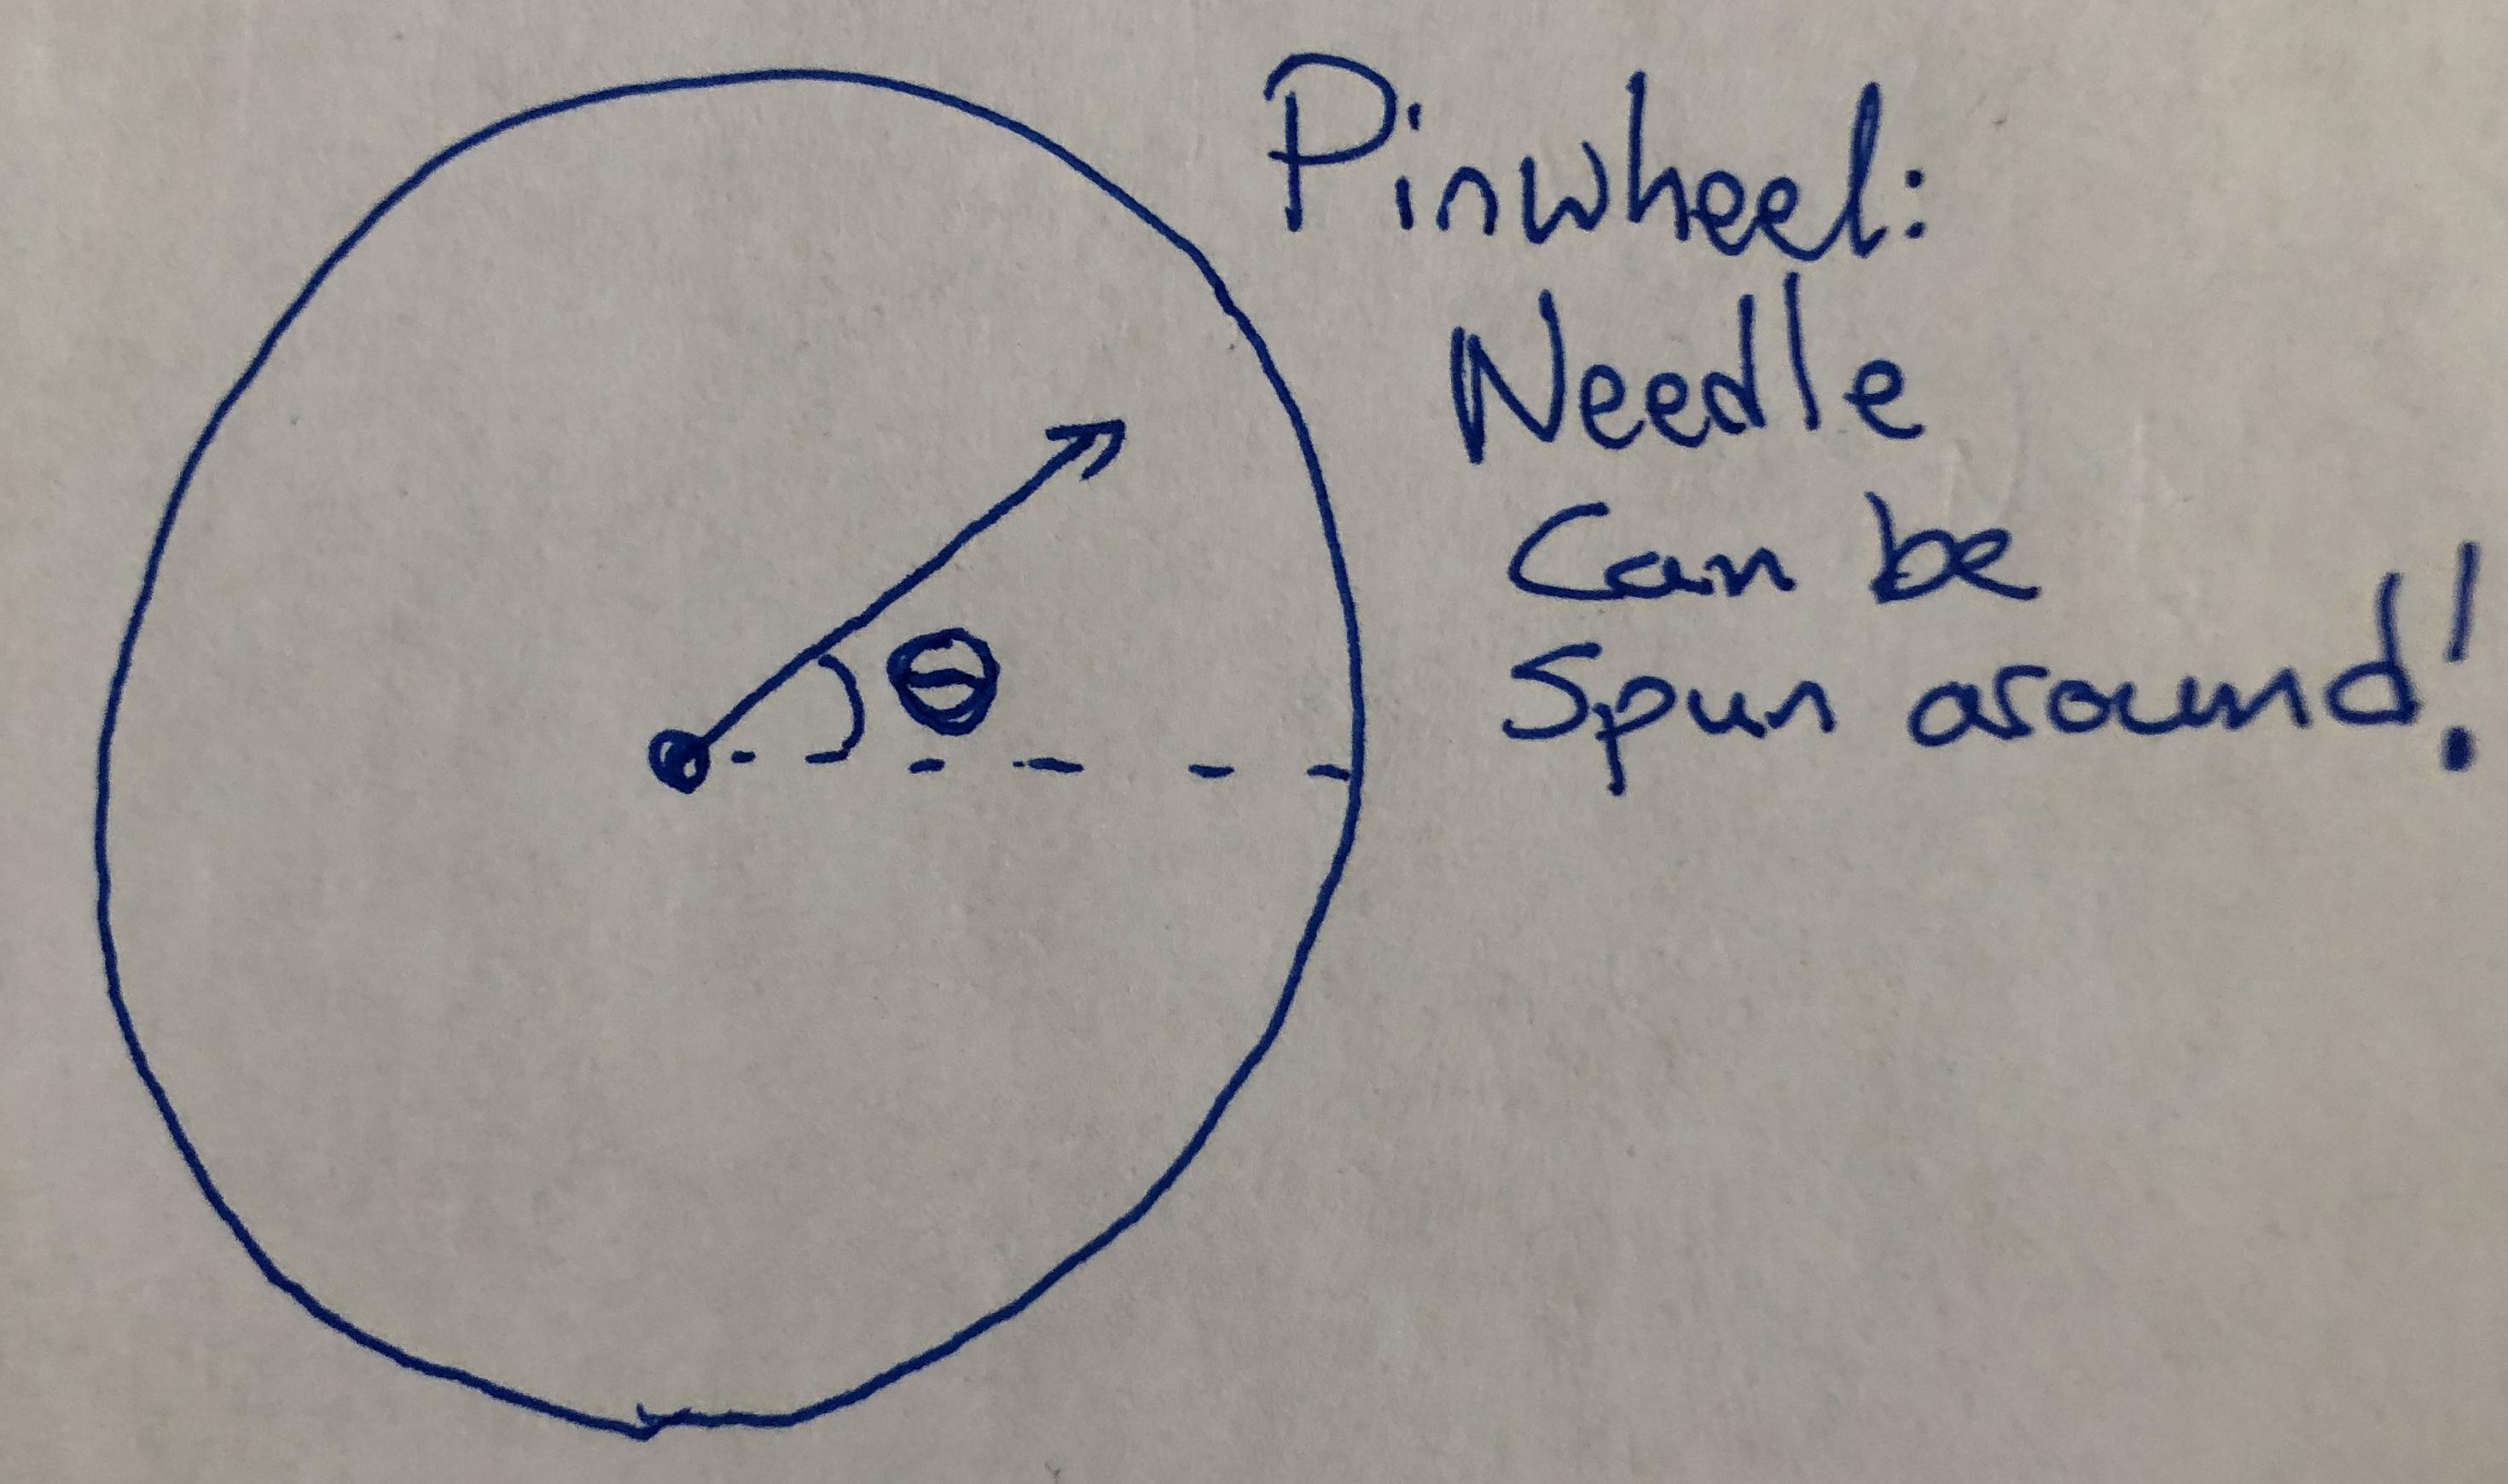
\includegraphics[scale=0.08]{images/pinwheel}
  \end{center}

  Suppose we spin the needle. When the needle stops spinning, we measure its
  angle from the dotted line. Let $X$ be the angle of the needle. So $X$ is a
  random variable. If $X$ is measured in degrees, then
  \begin{equation*}
    X \in  [0,360)
  \end{equation*}
  but $A$ could take \textit{any} value, not just integer values. On the other hand, if we measure $X$ in
  radians, then
  \begin{equation*}
    X\in [0,2\pi).
  \end{equation*}
  Moreover we have no reason to believe any one angle is more likely than any others -- for our idealized
  pinwheel, all values between $0$ and $2\pi$ should all be equally likely.
\end{example}

\begin{definition}[pdf]
  Let $X$ be a continuous random variable. The \demph{probability density function} (aka ``pdf'' or
  ``density'') of $X$ is a function $f_{X}$ such that for any real
  numbers $a,b$ with $a \leq b$, we have
  \begin{equation*}
    \P\left[X\in (a,b ) \right] = \int_{a}^{b} f_{X}(x)dx
  \end{equation*}
  The graph of $f_{X}$ is called the \demph{density curve} of $X$.
\end{definition}

\newpage
\section{2026-03-06 | Week 08 | Lecture 19}

\subsection{Continuous random variables}
\textit{(This lecture is based on sections 4.1-4.3 in the textbook)}

\begin{definition}[pdf]
  Let $X$ be a continuous random variable. The \demph{probability density function} (aka ``pdf'' or
  ``density'') of $X$ is a function $f$ such that for any real
  numbers $a,b$ with $a \leq b$, we have
  \begin{equation*}
    \P\left[X\in (a,b ) \right] = \int_{a}^{b} f(x)dx
  \end{equation*}
  The graph of $y=f(x)$ is called the \demph{density curve} of $X$.
\end{definition}

\Fl{Observatioins about pdfs:}
\begin{itemize}
  \item $f(x) \geq 0$ for all $x$
  \item $\int_{-\infty}^{\infty}f(x) dx= 1 $
  \item $f(x)$ is not a probability because it could be greater than 1.
  Insteady, you can think of it vaguely as a ``relative likeliood''.
\end{itemize}

\begin{proposition}
  Let $F(x) = \P\left[X \leq x\right]$ be the cdf of $X$, and let $f$ be the
  pdf of $X$. Then
  \begin{equation*}
    F(x) = \int_{-\infty}^{x}f(t)dt
    \quad \text{and} \quad 
    F'(x) = f(x)
  \end{equation*}
\end{proposition}

\begin{proposition}[Properties of cdfs of uniform random variables]
  \begin{itemize}
    \item []
    \item $\P\left[a \leq X \leq b\right] = F(b)-F(a)$
    \item $F$ is a nondecreasing function
    \item  $F(-\infty)=0$ and $F(+\infty)=1$.
  \end{itemize}
\end{proposition}



\begin{example}[Pinwheel example continued]
  Recall the example of the pinwheel \cref{ex:pinwheel}, with the angle $X$ measured in radians, so that
  the state space of $X$ is $[0,2\pi)$, with all values equally likely. Recall that we computed the pdf as
  \begin{equation*}
    f_{X}(x) = \frac{1}{2\pi}\cdot\mathbf{1}_{[0,2\pi)}(x) = \left\{ \begin{array}{l@{\quad:\quad}l} \frac{1}{2\pi} & x\in [0,2\pi)\\0 &x\notin [0,2\pi) \end{array}\right.
  \end{equation*}
  \begin{center}
    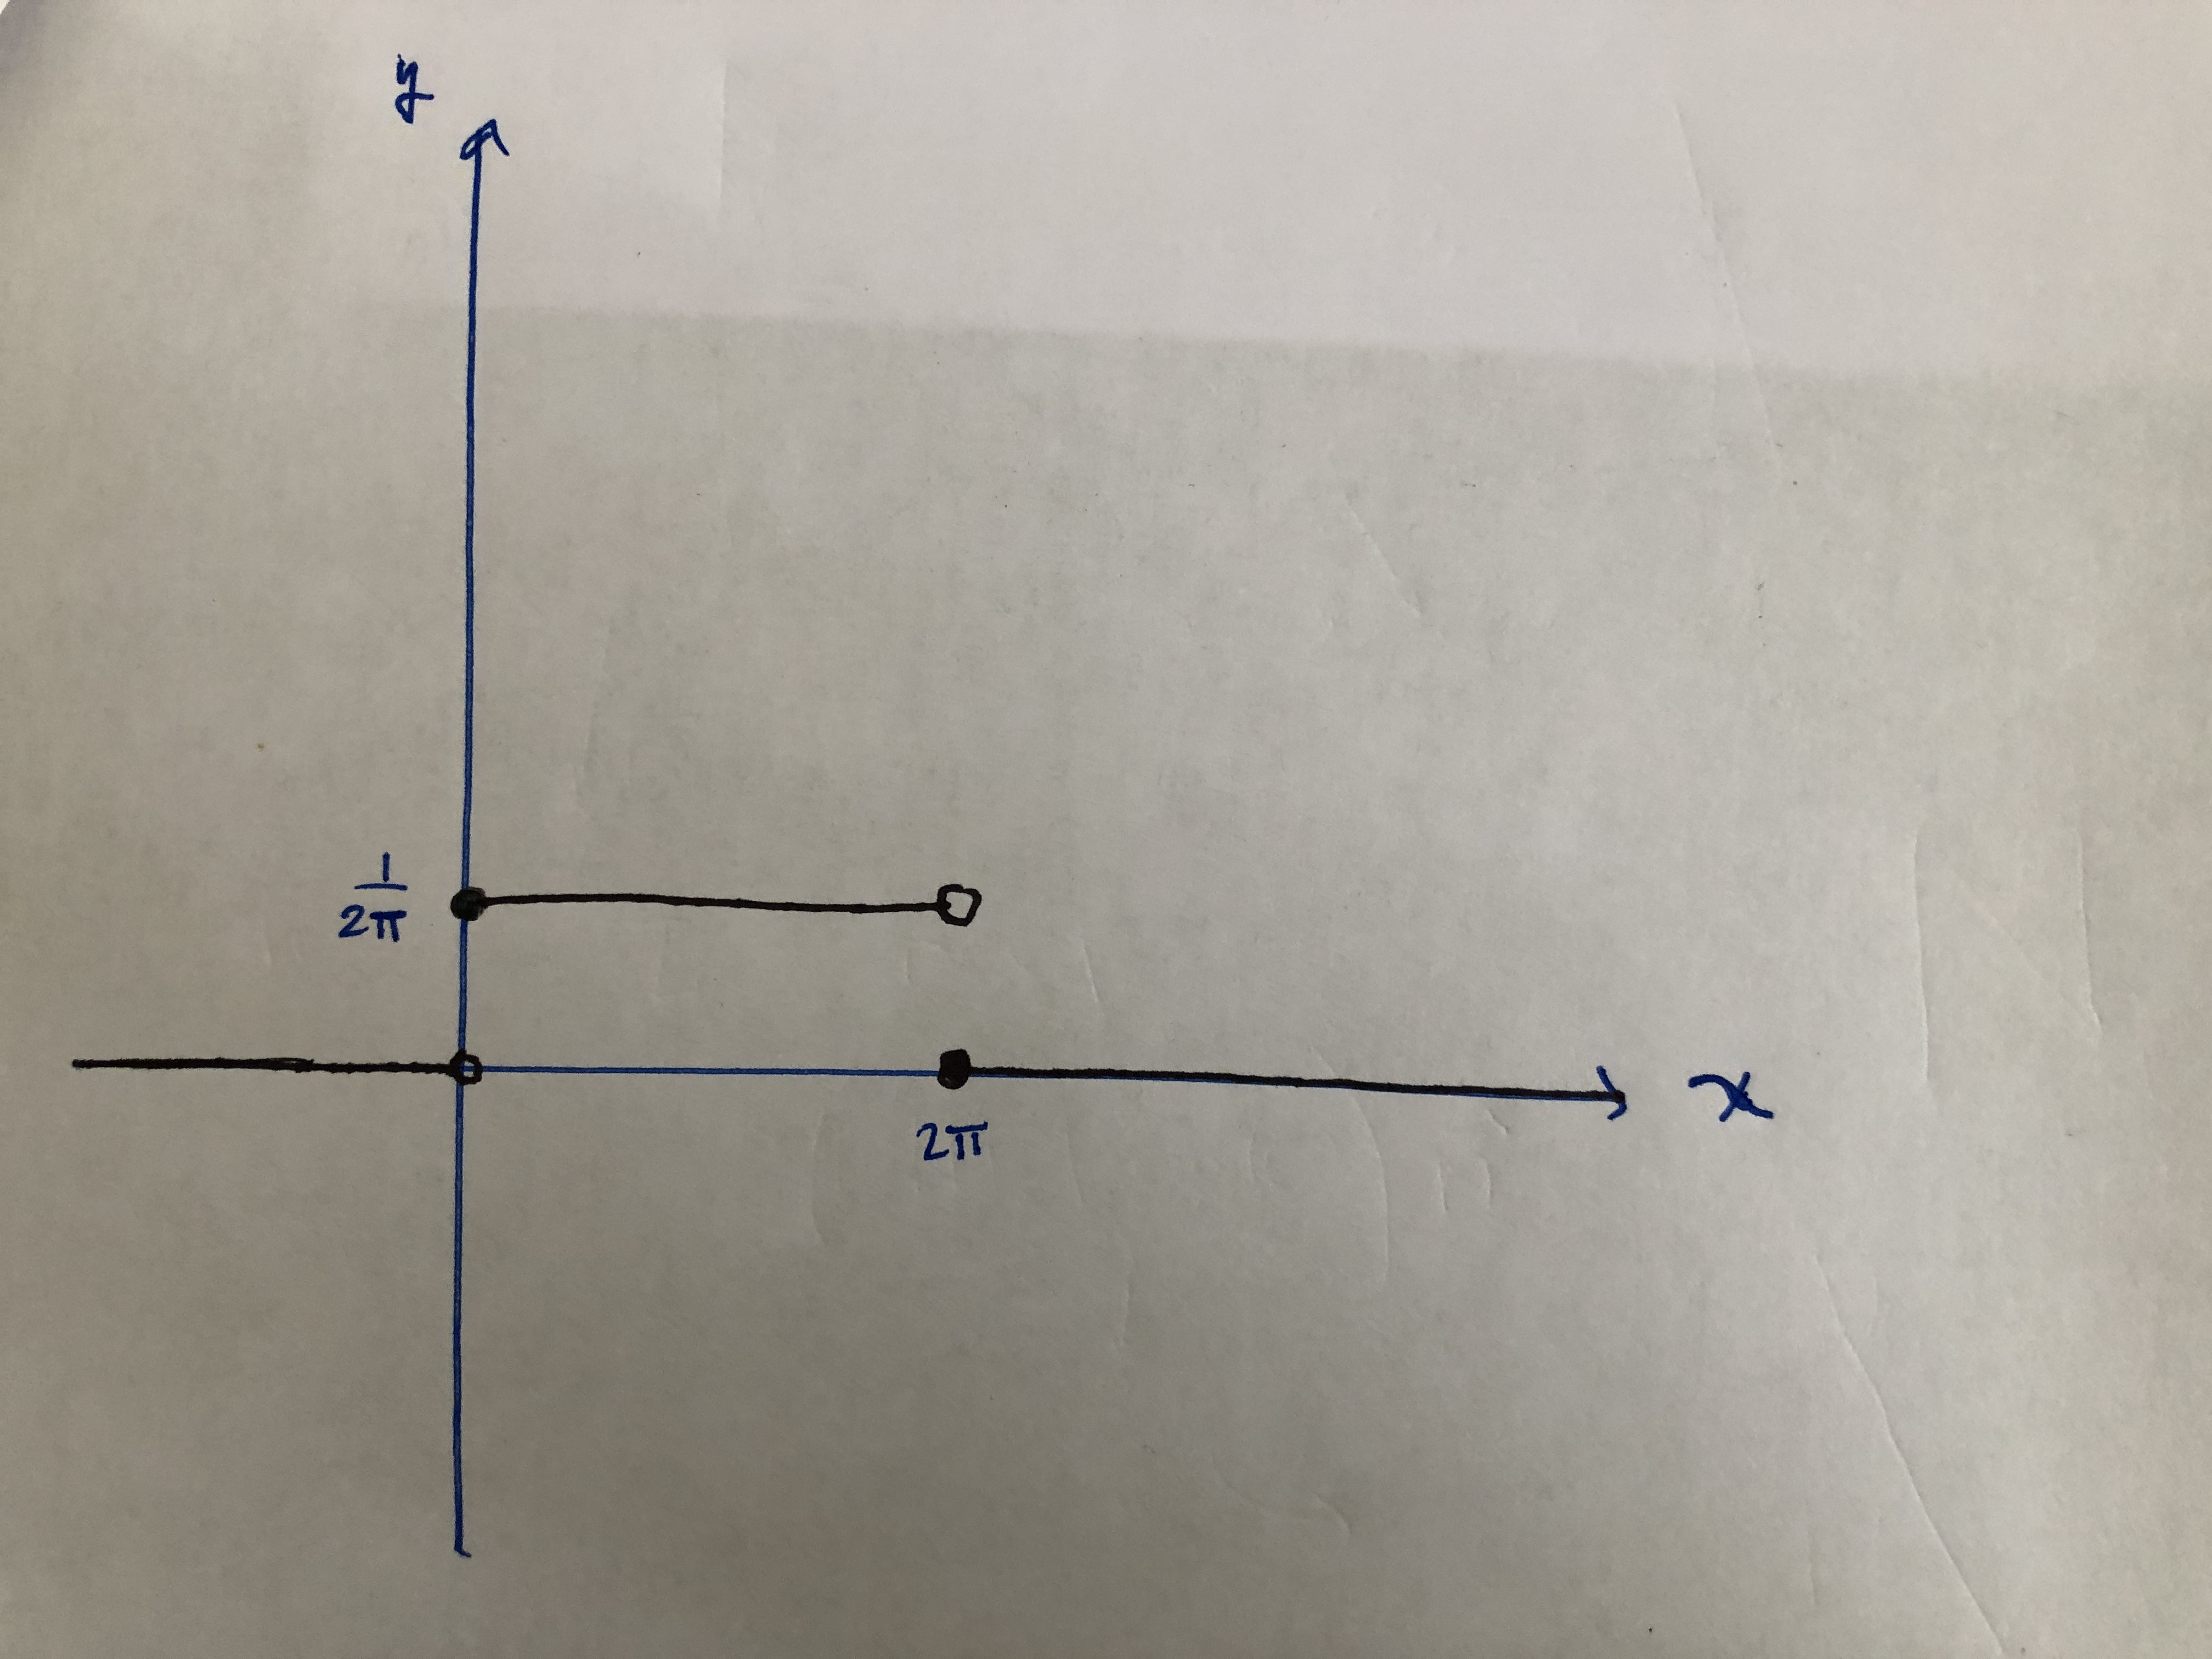
\includegraphics[scale=.045]{images/pinwheel-density-curve}
  \end{center}
  Recall also that the cdf is defined as
  \begin{equation*}
    F_{X}(x) := \int_{-\infty}^{x}f_{X}(t)dt.
  \end{equation*}
  So that for the pinwheel angle $X$, we have
  \begin{align}\label{eq:10}
    F_{X}(x) 
    &= \int_{-\infty}^{x} \frac{1}{2\pi}\cdot \mathbf{1}_{[0,2\pi)}(t)dt\nonumber\\
    &= \frac{1}{2\pi}\int_{-\infty}^{x}  \mathbf{1}_{[0,2\pi)}(t)dt.
  \end{align}
  To evaluate an integral of this form, we have to consider three cases:
  \begin{itemize}
    \item $x < 0$ (i.e. when $x$ is to the left of the interval)
    \item $x \geq 2\pi$ (i.e. when $x$ is to the right of the interval)
    \item $0 \leq x<2\pi $ (i.e. when $x$ is in the interval)
  \end{itemize}
  Let's think through these cases:
  \begin{itemize}
    \item When $x<0$, the integral on the right-hand side of \cref{eq:10} is
    zero.
    \item When $x \geq 2\pi$, the integral equals
    \begin{equation*}
      \int_{-\infty}^{0}0dt + \frac{1}{2\pi}\int_{0}^{2\pi} dt + \int_{2\pi}^{x}0dt = 0+1+0=1 
    \end{equation*}
    \item When $0 \leq x<2\pi$, the integral equals
    \begin{equation*}
      \int_{-\infty}^{0}0dt+ \frac{1}{2\pi}\int_{0}^{x} dt =0+ \frac{x}{2\pi} = \frac{x}{2\pi}
    \end{equation*}
  \end{itemize}
  From this analysis and \cref{eq:10}, we can conclude that
  \begin{equation*}
    F_{X}(x) = \left\{ \begin{array}{l@{\quad:\quad}l}
        0 & x < 0\\
        \frac{x}{2\pi} & 0 \leq x<2\pi\\
        1 & x \geq 2\pi \end{array}\right.
  \end{equation*}

  \begin{center}
    \begin{tikzpicture}
      % Axes
      \draw[->] (-2,0) -- (6,0) node[right] {$x$};%
      \draw[->] (0,-0.4) -- (0,2.2) node[above] {Probability};%
      
      % Function segments
      \draw[thick,blue,<-] (-2,0) -- (0,0);% % f(x) = 0 for x < 0
      \draw[thick,blue] (0,0) -- (3.14,1);% % f(x) = x / (2π) for 0 ≤ x ≤ 2π
      \draw[thick,blue,->] (3.14,1) -- (6,1);% % f(x) = 1 for x > 2π

      % tick marks
      \draw (-0.1,1) -- (0.1,1); % Tick at y = 1
      \draw (3.14,0.1) -- (3.14,-0.1); % Tick at x = π
      % Labels
      \node[below] at (0,-0.4) {$0$};%
      \node[below] at (3.14,0) {$2\pi$};%
      \node[left] at (0,1) {$1$};%
    \end{tikzpicture}
  \end{center}
\end{example}


\begin{definition}[Uniform random variable]
  \label{def:uniform-random-variable}
  Let $I$ be an interval with endpoints $a$ and $b$, such that $a<b$. A continuous random variable $X$
  has \demph{uniform distribution} on $I$ if it has pdf
  \begin{equation*}
    f(x) = \left\{ \begin{array}{l@{\quad:\quad}l} \frac{1}{b-a} & x\in I\\0 & x\notin I \end{array}\right.
  \end{equation*}
  In this case, $X$ is called a \demph{uniform} random variable.
\end{definition}

\begin{definition}[Exponential random variable]
  \label{def:exponential-random-variable}
  We say that $X$ is an \demph{exponential} random variable with rate
  $\lambda>0$ if it has pdf
  \begin{equation*}
    f(x)= \lambda e^{-\lambda x}\mathbf{1}_{\left[ x \geq 0\right]}.
  \end{equation*}
\end{definition}

\begin{remark}
  In \cref{def:exponential-random-variable}, the term
  $\mathbf{1}_{\left[ x \geq 0 \right] }$ is an ``indicator function'' which takes value $1$ when
  $x \geq 0$ and $0$ if $x<0$. 
\end{remark}

\newpage
\section{2026-03-09 | Week 09 | Lecture 20}

\subsection{Continuous random variables}
\begin{example}[Waiting times]
  \label{ex:waiting-times}
  Suppose you station yourself at spot on a road and watch as cars pass by. Let $T$ be the time in
  minutes until the first car passes by. This random variable is called the \textit{waiting time}.

  Under certain circumstances, it is reasonable for $T$ to have pdf
  \begin{equation}
    \label{eq:exponential-density}
    f(x) = \lambda e^{-\lambda x}\mathbf{1}_{\left[ x \geq 0 \right] }
  \end{equation}
  for a certain (fixed) value of $\lambda>0$.

  For concreteness, let's assume that $\lambda=3$, so
  \begin{equation*}
    f(x) = 3e^{-3x} \mathbf{1}_{\left[ x \geq 0\right] }
  \end{equation*}
  Then the cdf is
  \begin{align*}
    F(t) 
    &= \int_{-\infty}^{t}f_{T}(x)dx\\
    &= \int_{0}^{t}3 e^{-3 x}dx\\ 
    &=3 \left[ \frac{-e^{-4 x}}{3} \right]^{t}_{0}\\
    &= 1-e^{-3t}.
  \end{align*}
  Equivalently,
  \begin{equation*}
    \P\left[T>t \right] = e^{-3t}.
  \end{equation*}
  For example the probability that you have to wait more than $t=30$ seconds for a car to pass by is
  \begin{equation*}
    \P\left[T>5 \right] = e^{-3\cdot 0.5}\approx .22
  \end{equation*}
  What about
  \begin{equation*}
    \E\left[T \right]?
  \end{equation*}
  If the cars come at a rate of $\lambda=3$ cars per minute, then on average how long would you have to
  wait for a car to arrive? This should be $20$ seconds.

  % Let's do the calculation and check:
  % \begin{align*}
  %   \E\left[T \right] 
  %   &=\int_{-\infty}^{\infty} x f_{T}(x) dx\\
  %   &= \int_{0}^{\infty}3xe^{-3x}dx\\ 
  %   &= \int_{0}^{\infty}3x \frac{d}{dx}\left[ -\frac{1}{3}e^{-3x} \right]dx\\  
  %   &= \left[ \left( 3x \right)\left( -\frac{1}{3}e^{-3x} \right) \right]^{\infty}_{0}  - \int_{0}^{\infty} \frac{d}{dx}\left[ 3x \right] \left( -\frac{1}{3}e^{-3x} \right)dx\\     
  %   &= \int_{0}^{\infty} e^{-3x}dx\\
  %   &= \left[ -\frac{1}{3}e^{-3x} \right]^{\infty}_{0}\\
  %   &= 0 - (-\frac{1}{3})\\
  %   &= \frac{1}{3}\\
  %   &= 20 \text{ seconds}
  % \end{align*}
  % So if the rate of cars coming is $\lambda=3$ cars per minute, then on average, we'll have to wait 20
  % seconds.
\end{example}

\begin{definition}[Expected value -- continuous random variables]
  \label{def:expected-value-continuous-random-variables}
  The \demph{expected value} of a continuous random variable $X$ is 
  \begin{equation*}
    \E\left[X \right] := \int_{-\infty}^{\infty}xf(x)dx 
  \end{equation*}
  where $f(x)$ is the pdf of $X$. (Provided that the integral above converges absolutely).
\end{definition}

We also have an analogue of the law of the unconscious statistician
(\cref{thm:LOTUS-discrete-case})

\begin{theorem}[LOTUS - continuous case]
  \label{thm:lotus-continuous-case}
  Let $X$ be a continous random variable with pdf $f$. Then for any function
  $h:\R \to \R$,
  \begin{equation*}
    \E\left[h(X) \right]= \int_{-\infty}^{\infty}h(x)f(x)dx,
  \end{equation*}
  provided that the integral exists and is finite.
\end{theorem}


Suppose $\mu= \E\left[X \right]$. Applying \cref{thm:lotus-continuous-case} to
the function $h(x)= (x- \mu)^{2}$ gives the following formula for the variance
of a continuous random variable:
\begin{equation*}
  \Var(X) := \E\left[(X-\mu)^{2} \right]=\int_{-\infty}^{\infty}(x-\mu)^{2}f(x)dx.
\end{equation*}

And again, we have the shortcut formula
\begin{equation*}
  \Var(X) = \E\left[X^{2} \right]- \left( \E\left[X \right] \right)^{2} .
\end{equation*}

\section{2026-03-11 | Week 09 | Lecture 21}

\subsection{Normal random variables}
\textit{This section is based on chapter 4.3}.


\begin{definition}[Normal / Gaussian Distribution]
  \label{def:gaussian-distribution}
  A random variable $X$ is said to be \demph{normally distributed} with mean
  $\mu\in \R$ and variance $\sigma^{2}>0$ if it has pdf
  \begin{equation*}
    f(x) = \frac{1}{\sqrt{2\pi\sigma^{2}}}
    \exp\left(-\frac{(x-\mu)^{2}}{2\sigma^{2}} \right),
  \end{equation*}
  defined for all $x\in \R$. We abbreviate this by writing
  $X\sim \mathcal{N}(\mu,\sigma^{2})$. If $X\sim \mathcal{N}(0,1)$, we say $Y$
  has \demph{standard normal distribution}. The parameter $\sigma$ is called
  the \demph{standard deviation} of $X$, and is the positive square root of
  the variance.
\end{definition}

\begin{remark}[Notation]
  \begin{itemize}
    \item []
    \item It is a common convention to denote a standard normal random
    variable with the letter $Z$.
  
    \item random variables/distributions are also called \demph{Gaussian}
    random variables/distributions.
  \end{itemize}
\end{remark}

\begin{example}
  Normal distributions are the classic ``bell curve'' distributions. Whenever
  a random quantity is the result of adding up many small, independent random
  effects, we expect it to be approximately normally distributed.

  \begin{itemize}
    \item A classic example is human height, which is influenced by the
    combined effects of thousands of genes together with environmental
    factors.
    \item Another example is repeated measurements of the same physical
    quantity (e.g., if we all went out and measured the temperature outside
    tomorrow at midday), this is because the total error is the sum of many
    small independent sources of noise (e.g., instrument precision, time,
    location, shade, wind, etc).
  \end{itemize}
\end{example}


\begin{remark}[Standardization]
  \label{rmk:standardization}
  If $Y \sim \mathcal{N}(\mu,\sigma^{2})$ then the random
  variable
  \begin{equation*}
    Z = \frac{X-\mu}{\sigma}
  \end{equation*}
  is a standard normal random variable (i.e., $Z\sim \mathcal{N}(0,1)$. The transformation
  \begin{equation*}
    X \mapsto \frac{X-\mu}{\sigma}
  \end{equation*}
  in which we subtract off the mean of $X$ and then divide by its standard
  deviation is called \demph{standardization}.
\end{remark}

\begin{remark}[The Empirical Rule]
  \label{rmk:empirical-rule}
  The \textbf{Empirical Rule} (also called the \textbf{68-95-99.7 rule}; see
  textbook section 1.3) is summarized by the following figure, for normal
  distributions:
  \begin{center}
    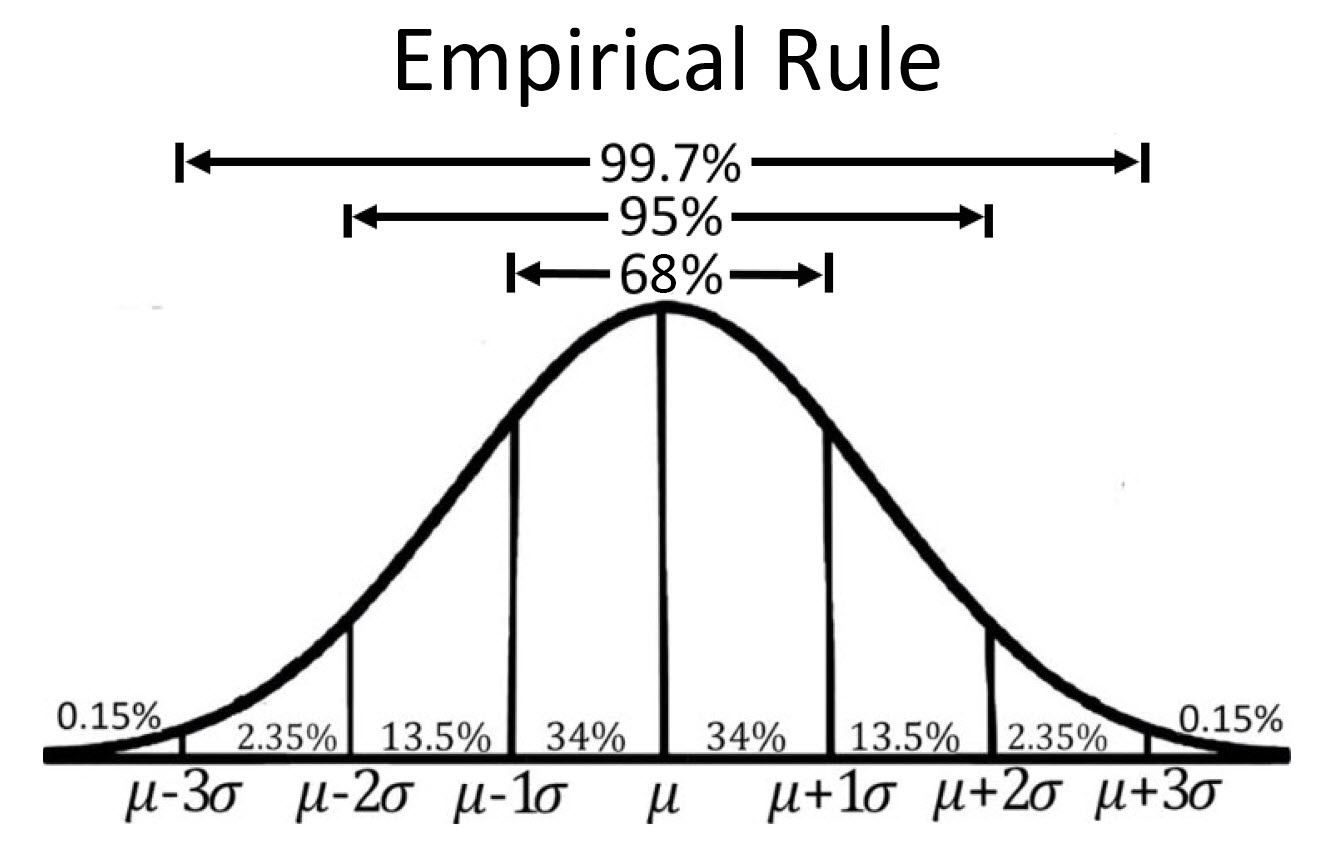
\includegraphics[scale=.25]{images/empirical-rule-normdist2.jpg}
    
    \textit{\tiny Image source: \url{https://andymath.com/wp-content/uploads/2019/12/empirical-rule-normdist2.jpg}}
  \end{center}
\end{remark}

\begin{remark}
  Note that $\mu$ determines where the peak of the bell curve is
  located, and $\sigma$ determines how wide or narrow it is.
\end{remark}
% Normal random variables have a ``bell-curve'' distribution. Here are some example density curves for
% various values of $\mu$ and $\sigma$. Note that $\mu$ determines where the peak of the bell curve is
% located, and $\sigma$ determines how wide or narrow it is:
% \begin{center}
%   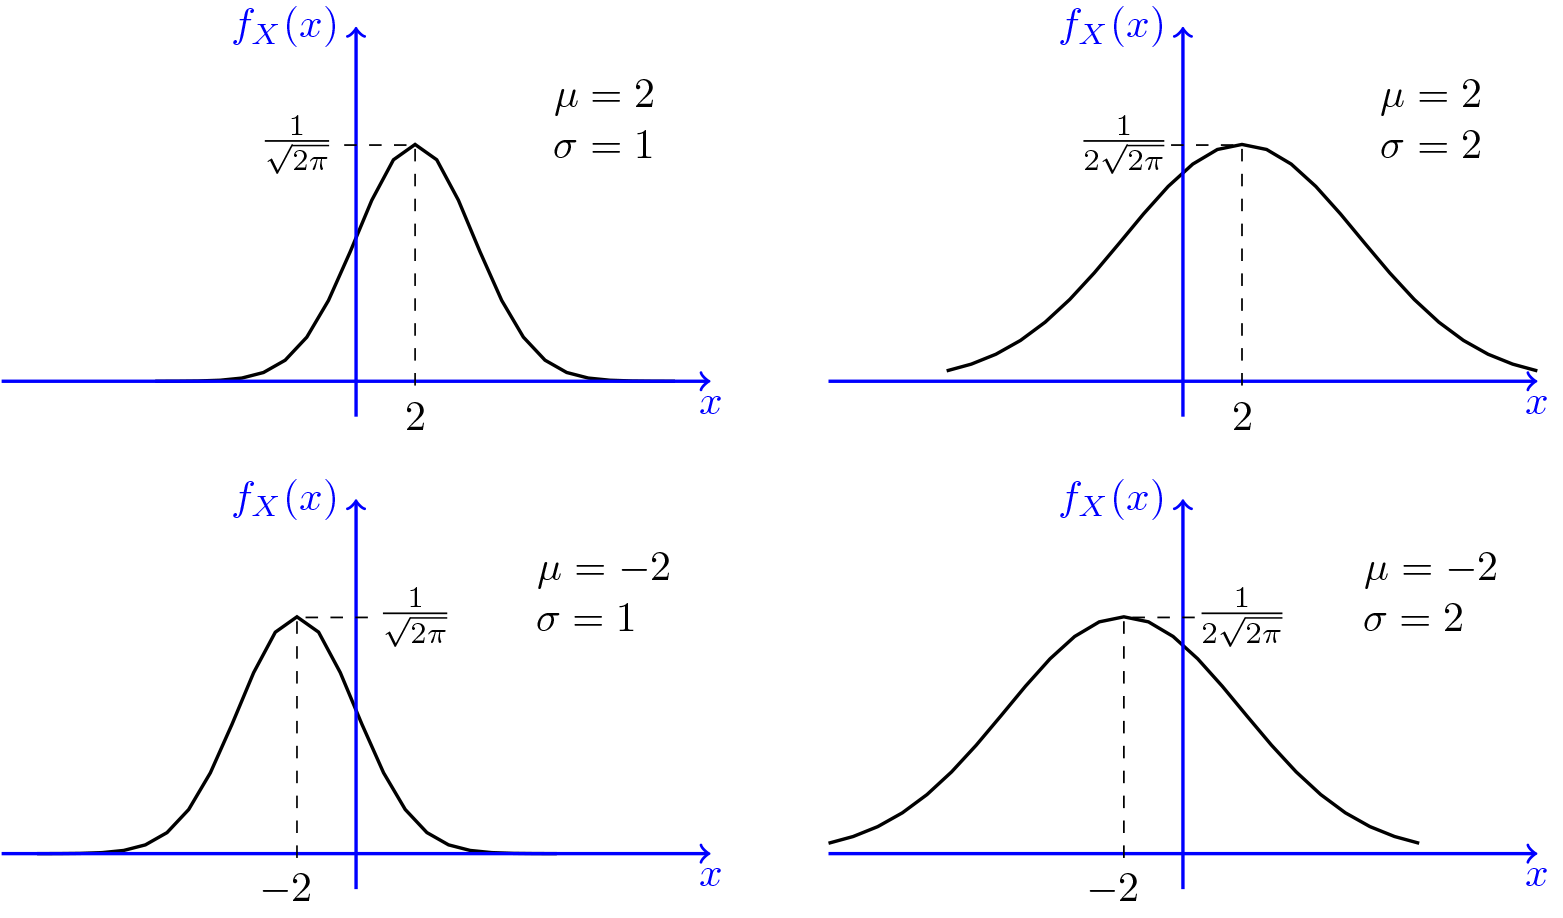
\includegraphics[scale=1]{images/some-normal-density-curves}
%   % picture taken from https://www.probabilitycourse.com/chapter4/4_2_3_normal.php
% \end{center}

% \Fl{Most important special case:} The most important special case is where $\mu=0$ and $\sigma^{2}=1$, in which
% case the density is
% \begin{equation*}
%   \phi(x) = \frac{1}{\sqrt{2\pi}}e^{-\frac{x^{2}}{2}} \quad -\infty<x<\infty
% \end{equation*}
% A random variable with this density is called a \demph{standard normal} and is usually denoted with the
% letter $Z$.


% But first, we should really check that $\phi$ is really a density. Namely, we
% need to check that
% \begin{equation*}
%   \int_{-\infty}^{\infty}\phi(x)dx = 1. 
% \end{equation*}

% We showed how to do this by using Fubini's theorem and converting to polar coordinates.


% \Fl{The CDF of a standard normal:} The cdf of a standard normal is usually denoted with the symbol
% $\Phi$:
% \begin{equation*}
%   \Phi(x) = \int_{-\infty}^{x}\phi(u)du  = \frac{1}{\sqrt{2\pi}}\int_{-\infty}^{x} e^{-\frac{u^{2}}{2}}du. 
% \end{equation*}
% There is no elementary form for the antiderivative $\Phi$, so generally we
% compute the values with a computer.


The next example shows how we can use standardization to do calculations:

\begin{example}
  Due to variation in the manufacturing process, the peak power consumption $X$ of
  the latest Nvidia GPU varies slightly from chip to chip. Assume the power
  consumption is normally distributed $X\sim \mathcal{N}(\mu,\sigma^{2})$. What
  is the probability that $X$ is within one standard deviation of its mean?

  \begin{align*}
    \P\left[\mu-\sigma \leq X \leq \mu+\sigma\right]
    &= \P\left[ \frac{(\mu-\sigma)-\mu}{\sigma}\leq \frac{X-\mu}{\sigma} \leq \frac{(\mu+\sigma)-\mu}{\sigma}\right]\\
    &= \P\left[ \frac{(\mu-\sigma)-\mu}{\sigma}\leq Z \leq
      \frac{(\mu+\sigma)-\mu}{\sigma}\right] &&\text{by \cref{rmk:standardization} }\\
    &= \P\left[-1 \leq Z \leq 1\right]\\
    &= \int_{-1}^{1}\frac{1}{\sqrt{2 \pi}} e^{-\frac{x^{2}}{2}}dx\\
    &\approx .68 &&\text{using the figure in \cref{rmk:empirical-rule}}
  \end{align*}
  So if $\mu=700$ watts and $\sigma= 35$ watts (realistic values for the
  Nvidia's new \$30,000 H100 GPU), we have
  \begin{equation*}
    \P\left[665 \leq X \leq 735\right]\approx 0.68.
  \end{equation*}
  In other words, about 68\% of chips will have peak power consumption between
  665 and 735 watts.
\end{example}

\newpage
\section{2026-03-23  | Week 10 | Lecture 22}
\subsection{Joint distributions - discrete case}
\label{sec:joint-distributions-discrete-case}
\textit{Please read chapter 5.1}

We are interested in understanding the properties of \demph{random vectors}, which are vectors whose
entries are random variables. We'll start with the case where the random
variables are discrete.


\begin{definition}[Joint pmf]
  Let $X$ and $Y$ be two discrete random variables. The \demph{joint pmf} of
  $X$ and $Y$ is the function
  \begin{equation*}
    p(x,y) = \P\left[X=x,Y=y \right],
  \end{equation*}
  defined for all $x,y\in \R$.
\end{definition}

\begin{remark}
  \begin{itemize}
    \item[]
    \item It must be the case that $p(x,y) \geq 0$ and
    $\sum_{x,y}p(x,y)=1$.
    \item Let $A$ be any set consisting of pairs of $(x,y)$ values. Then the
    probability
    \begin{equation*}
      \P\left[(X,Y)\in A\right] = \sum_{(x,y)\in A} p(x,y)
    \end{equation*}
  \end{itemize}
\end{remark}

\begin{example}
  Cars made in a factory experience two kinds of defects: defective joint welds, and and improperly
  tightened bolts. Let
  \begin{itemize}
    \item $X = $ number of defective welds in a new car
    \item $Y = $ number of improperly tightened bolts
  \end{itemize}
  Past data suggests that the joint pdf of $(X,Y)$ is given by the following table:
  \begin{center}
    \begin{tabular}{ll|llll}
      &   & & \quad Y    \\
      &   & 0   & 1    & 2    & 3    \\ \hline
      & 0 & .840 & .030  & .020  & .010  \\
      X& 1 & .060 & .010  & .008 & .002 \\
      & 2 & .010 & .005 & .004 & .001
    \end{tabular}
  \end{center}
  The probability that there are no defects in the car is
  \begin{equation*}
    p(0,0) = \P\left[X=0,Y=0 \right] = .84
  \end{equation*}
  The probability that there will be exactly one defect is
  \begin{equation*}
    p(0,1)+p(1,0) = \P\left[X=0,Y=1 \right]+ \P\left[X=1,Y=0 \right] = .06+.03 = .09.
  \end{equation*}
  What is the probability that there will be no improperly tightened bolts? This concerns only the
  variable $Y$. This can be obtained by summing  over all values of $x$:
  \begin{align*}
    \P\left[Y=0 \right] 
    &= \sum_{x=0}^{2}\P\left[X=x, Y=0 \right]\\
    &= p(0,0)+p(1,0)+p(2,0)\\
    &= .84+.06+.01\\
    &= .91
  \end{align*}
\end{example}

Given the joint pmf for a two-dimensional discrete random vector $(X,Y)$, it
is easy to derive the individual pmfs for $X$ and $Y$, and in this context we
call them ``marginal pmfs''. The manner in which this is done is suggested by
the previous example.

\begin{definition}
  If $p(x,y)$ is the pmf of $(X,Y)$, then the \demph{marginal pmf} of $X$ is
  \begin{equation*}
    p_{X}(x)=  \P\left[X=x \right] = \sum_{\text{all }y}p(x,y).
  \end{equation*}
  Similary, the \demph{marginal pmf} of $Y$
  \begin{equation*}
    p_{Y}(y) = \P\left[Y = y \right] = \sum_{\text{all } x}p(x,y).
  \end{equation*}
\end{definition}
Recall that two events are independent if knowledge that one has occurred
gives no information about whether the other has occurred. We can extend this
idea to random variables:
\begin{definition}[Independence of rvs - discrete case]
  Let $X,Y$ be discrete random variables with joint pmf $p(x,y)$. We say that
  $X$ and $Y$ are \demph{independent} if for every pair of $(x,y)$-values,
  \begin{equation*}
    p(x,y) = p_{X}(x)\cdot p_{Y}(y)
  \end{equation*}
  If this condition isn't satisfied for all $(x,y)$, then $X$ and $Y$ are said to be \demph{dependent}.
\end{definition}

The intuition is this: two random variables are independent if observing one of them doesn't give you any
information about the other. 

\begin{example}
  In the car factory example, $X$ and $Y$ have with joint pmf is specified by
  the table
  \begin{center}
    \begin{tabular}{ll|llll}
      &   & & \quad Y    \\
      &   & 0   & 1    & 2    & 3    \\ \hline
      & 0 & .840 & .030  & .020  & .010  \\
      X& 1 & .060 & .010  & .008 & .002 \\
      & 2 & .010 & .005 & .004 & .001
    \end{tabular}
  \end{center}
  where, for example $p(1,3) = .002$.
  
  The marginal pmfs are given by the following tables:
  \begin{center}
    \begin{tabular}{l|l}
      $x$ & $p_X(x)$\\ \hline
      0& .9\\
      1& .08\\
      2& .02\\
    \end{tabular}
    \quad \text{and} \quad
    \begin{tabular}{l|l}
      $y$ & $p_Y(y)$\\ \hline
      0& .91\\
      1& .045\\
      2& .032\\
      3& .013\\
    \end{tabular}
  \end{center}
  Are $X$ and $Y$ independent? Having computed the pmfs, we can verify that
  $X$ and $Y$ are \textbf{not independent}. This is because
  \begin{equation*}
    p(0,0) = .84 \neq (.9)(.91) = .819 = p_{X}(0)p_{Y}(0).
  \end{equation*}
\end{example}

\subsection{Joint distributions - continuous case}

\textit{Based on chapter 5.1 in the textbook -- in particular, please read
  examples 5.5 and 5.14 in the textbook.}

The theory for continuous random vectors parallels closely the theory for
discrete random variables presented in \cref{sec:joint-distributions-discrete-case}.

\begin{definition}
  If $X,Y$ are continuous r.v.s, then the \demph{joint pdf} $f(x,y)$ is a
  function satisfying $f(x,y) \geq 0$ and
  $\int_{-\infty }^{\infty}\int_{-\infty}^{\infty}f(x,y)dxdy=1$ such that for
  any 2-dimensional set $A$,
  \begin{equation*}
    \P\left[(X,Y)\in A \right] = \int_{A}\int f(x,y)dxdy
  \end{equation*}
  The \demph{marginal densities} of $X$ and $Y$ are
  \begin{equation*}
    f_{X}(x) = \int_{\text{all }y} f(x,y)dy \quad \text{and} \quad f_{Y}(y) = \int_{\text{all }x} f(x,y)dx
  \end{equation*}
  We say that $X$ and $Y$ are \demph{independent} if
  \begin{equation*}
    f(x,y) = f_{X}(x)\cdot f_{Y}(y).
  \end{equation*}
  for all $x,y\in \R$.
\end{definition}

\newpage
\section{2026-03-25 | Week 10 | Lecture 23}

\subsection{An example of using a joint distribution to compute probabilities}
\begin{example}
  Let $X$ and $Y$ be the lifetimes of two lightbulbs, in months. Assume that
  the expected lifetimes are 10 months and 12 months, respectively. Also
  assume that the lifetimes are independent, exponentially-distributed random variables.

  Then
  \begin{equation*}
    f_{X}(x) = \frac{1}{10} e^{-\frac{1}{10} x}\mathbf{1}_{[x>0]} \quad \text{and} \quad f_{Y}(y) = \frac{1}{12} e^{-\frac{1}{12} y}\mathbf{1}_{[y>0]}.
  \end{equation*}
  
  Since $X$ and $Y$ are independent, the joint pdf is
  \begin{align*}
    f(x,y) 
    &= f_{X}(x)f_{Y}(y)\\
    &= \left( \frac{1}{10} e^{-\frac{1}{10} x}\mathbf{1}_{[x>0]} \right) \left( \frac{1}{12} e^{-\frac{1}{12} y}\mathbf{1}_{[y>0]} \right)\\ 
    &= \frac{1}{120} e^{-\frac{1}{10} x-\frac{1}{12} y }\mathbf{1}_{[x,y>0]}\\
    &= \left\{ \begin{array}{l@{\quad:\quad}l} \frac{1}{120} e^{-\frac{1}{10}
          x-\frac{1}{12} y } & x>0 \text{ and }y>0\\ 0& \text{else}
      \end{array}\right.
  \end{align*}


  \textbf{Question:} What is the probability that both lightbulbs last at
  least 9 months?

  Want:
  \begin{align*}
    \P\left[X \geq 9, Y \geq 9\right]
    &= \int_{9}^{\infty} \int_{9}^{\infty} f(x,y)dxdy\\
    &= \int_{9}^{\infty} \int_{9}^{\infty} f_{X}(x) f_{Y}(y) dxdy\\
    &= \int_{9}^{\infty} \left[ \int_{9}^{\infty} f_{X}(x) f_{Y}(y) dx \right] dy\\
    &= \int_{9}^{\infty} \left[ \int_{9}^{\infty} f_{X}(x)  dx \right] f_{Y}(y)dy\\
    &= \left( \int_{9}^{\infty} f_{X}(x)dx \right)  \left( \int_{9}^{\infty} f_{Y}(y) dy \right) \\
    &= \left( \int_{9}^{\infty} \frac{1}{10}e^{-\frac{1}{10}x}dx \right)  \left( \int_{9}^{\infty} \frac{1}{12}e^{-\frac{1}{12}y}dy \right) \\
    &= \left[ -e^{\frac{1}{10}x} \right]^{x=\infty}_{x=9} \cdot \left[ -e^{\frac{1}{12}y} \right]^{y=\infty}_{y=9}\\  
    &=e^{-9 \left( \frac{1}{10}+\frac{1}{12} \right) }\\
    &=e^{-1.65}\\
    &\approx .2.
  \end{align*}
  So with probability about one fifth, both ligthbulbs will last at least 900 hours.

  % A faster way to do this. Observe that the events $\left[ X \geq 9\right]$ and $\left[ Y \geq
  %   9\right]$ are independent, because the random variables are. Then
  % \begin{align*}
  %   \P\left[X \geq 9, Y \geq 9\right] 
  %   &= \P\left[X \geq 9\right] \P\left[Y \geq 9\right]\\
  %   &= e^{-9 \alpha} e^{-9 \beta}\\
  %   &= e^{-1.65}
  % \end{align*}
\end{example}

\subsection{LOTUS Theorem - multivariate case}
\textit{Chapter 5.2 in the textbook.}

\begin{theorem}[LOTUS - multivariate case]
  \label{thm:LOTUS-multivariate-case}
  Let $X,Y$ be random variables with joint pmf $p(x,y)$ if $X,Y$ are discrete,
  or joint pdf $f(x,y)$ if $X,Y$ are continuous. Then for any function
  $h:\R^{2} \to \R$,
  \begin{equation*}
    \E\left[h(X,Y) \right] =\left\{ \begin{array}{l@{\quad:\quad}l}
        \displaystyle\sum_{\text{all }x,y} h(x,y)p(x,y) & \text{if $X,Y$ are discrete}\\
        \displaystyle \int_{-\infty}^{\infty}\int_{-\infty}^{\infty}h(x,y)f(x,y)dxdy   & \text{if $X,Y$ are continuous}
      \end{array}\right.
  \end{equation*}
\end{theorem}

An important aplication of \cref{thm:LOTUS-multivariate-case}:

\begin{theorem}
  \label{thm:independent-expectations-factorize}
  If $X,Y$ are indepenedent random variables then
  \begin{equation*}
    \E\left[XY \right] = \E\left[X \right] \E\left[Y \right]
  \end{equation*}
\end{theorem}
\begin{proof}
  Let's prove the case with $X,Y$ discrete. Let $p(x,y)$ be the joint pmf of
  $X$ and $Y$. Taking $h(x,y) = xy$, \cref{thm:LOTUS-multivariate-case} implies
  \begin{align*}
    \E\left[XY \right] 
    &= \sum_{\text{all }x,y} xyp(x,y)\\
    &= \sum_{\text{all }x,y} xyp_{X}(x) \cdot p_{Y}(y) &&\text{by independence}\\
    &= \left( \sum_{\text{all }x} xp_{X}(x) \right) \left( \sum_{\text{all }y}yp_{Y}(y)  \right)\\   
    &= \E\left[X \right] \E\left[Y \right] &&\text{by \cref{thm:LOTUS-discrete-case}}
  \end{align*}
  The continuous case is similar.
\end{proof}

One important function for \cref{thm:LOTUS-multivariate-case}  is when $h(X,Y) =
(X-\mu_{X})(Y-\mu_{Y})$, where $\mu_{X}= \E\left[X \right]$ and $\mu_{Y} = \E\left[Y \right]$. That gives
us a formula for what is called the \demph{covariance}:
\begin{equation*}
  \text{Cov}(X,Y) = \E\left[(X-\mu_{X})(Y-\mu_{Y}) \right]
\end{equation*}
By foiling this out, we get
\begin{equation*}
  \text{Cov}(X,Y) = \E\left[XY \right] - \mu_{X}\mu_{Y}
\end{equation*}
\fl{Interpetation:} covariance is a rough measure of the relationship between
the two random variables.
By \cref{thm:independent-expectations-factorize}, if $X,Y$ are independent, then
\begin{equation*}
  \text{Cov}(X,Y) = \E\left[XY \right] - \mu_{X}\mu_{Y} = \E\left[X \right] \E\left[Y \right] -\mu_{X}\mu_{Y} = 0.
\end{equation*}




\begin{example}[Covariance calculation]
  Let $X,Y$ be random variables with joint distribution
  \begin{equation*}
    f(x,y) = 24xy
  \end{equation*}
  whose domain is
  \begin{equation*}
    D:= \left\{(x,y)\in \R^{2}: x \geq 0, y \geq 0, x+y \leq 1\right\}
  \end{equation*}
  which is shown below:
  \begin{center}
    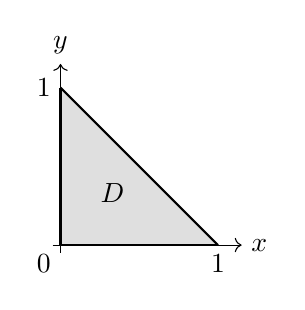
\begin{tikzpicture}[scale=2]
      % axes
      \draw[->] (-0.05,0) -- (1.15,0) node[right] {$x$}; \draw[->] (0,-0.05)
      -- (0,1.15) node[above] {$y$};

      % shaded region
      \fill[gray!25] (0,0) -- (1,0) -- (0,1) -- cycle;

      % boundary lines
      \draw[thick] (0,0) -- (1,0); \draw[thick] (0,0) -- (0,1); \draw[thick]
      (1,0) -- (0,1);

      % labels
      \node[below left] at (0,0) {$0$}; \node[below] at (1,0) {$1$};
      \node[left] at (0,1) {$1$}; \node at (0.33,0.33) {$D$};
    \end{tikzpicture}
  \end{center}
  \Fl{What is the covariance} To compute $\E\left[XY \right]$, let's take
  $h(x,y)=xy$. Recalling that $f(x,y) = 24xy$ for $(x,y)\in D$, we have
  \begin{align*}
    \E\left[XY \right] 
    &= \int_{D} h(x,y) f(x,y)dxdy \\
    &= \int_{D} (xy)24xy dxdy\\
    &= 24\int_{D} x^{2}y^{2}dxdy\\
    &= 24 \int_{0}^{1} \int_{0}^{1-y}  x^{2}y^{2}dxdy\\
    &= 24 \int_{0}^{1}y^{2} \left[\int_{0}^{1-y}x^{2} dx \right] dy\\
    &= 8 \int_{0}^{1}y^{2}(1-y)^{3}dy\\ 
    &= \ldots\\
    &= -8.
  \end{align*}
\end{example}

\newpage


\section{2025-03-27 | Week 10 | Lecture 24}

\subsection{Statistics: a general framework}

\textit{Chapters 5.3 and 5.4}


\textit{The objective of statistics to is to make an inference about a
  population based on information contained in a sample from that population
  and to provide an associated measure of goodness for the inference.} Here we
introduce a conceptual framework for mathematical statistics.


A \demph{population} is a large body of data that is the target of our
interest. The subset collected from it is our \demph{sample}. 

\begin{example}[Populations]
  A population can be real or theoretical. Here are some examples
  \begin{itemize}
    \item The set of people in Hawai{\okina}i (real, finite)
    \item The set of voters in the 2026 Midterm elections (hypothetical, finite)
    \item The decimal expansion of $\pi$ (countably infinite)
    \item The infinitely many observations that could be made during a
    laboratory experiment if the experiment were repeated over and over again
    (hypothetical)
    \item The lifetimes of light bulbs produced by a factory
  \end{itemize}
  Importantly, a population can also be a \textit{probability distribution},
  specified by a pdf, pmf, or cdf
  \begin{itemize}
    \item Observations made from an exponential distribution with rate $\lambda>0$ (i.e., the distribution with pdf $f(x)=\lambda e^{-\lambda x}\mathbf{1}_{\left[ x>0 \right] }$.)
  \end{itemize}
\end{example}


More commonly in mathematical statistics, we think of the population as a
distribution.

\begin{definition}[Random sample from a distribution]
  Consider a given probability distribution on $\R$ that can be represented by
  a pdf or pmf $f$. We say that the random variables $X_{1},\ldots,X_{n}$ form
  a \demph{random sample} from this distribution if these random variables are
  independent and the distribution of each is given by $f$. Such random
  variables are also said to be \demph{independent and identically
    distributed} (iid). The number of random variables $n$ is the
  \demph{sample size}.
\end{definition}


\subsection{What is a statistic?}
\begin{definition}[Statistic]
  A \demph{statistic} is any quantity whose value can be calculated from
  sample data.
\end{definition}

Here are two important examples of statistics:

\begin{example}
  Let $X_{1},\ldots,X_{n}$ be random sample.
  \begin{itemize}
    \item The \demph{sample mean}, denoted $\overline{X}$, is
    \begin{equation*}
      \overline{X}=\frac{X_{1}+\ldots+X_{n}}{n}.
    \end{equation*}
    \item The \demph{sample variance}, denoted $S^{2}$, is
    \begin{equation*}
      S^{2} = \frac{1}{n-1}\sum_{i=1}^{n}(X_{i} - \overline{X})^{2}
    \end{equation*}
  \end{itemize}
\end{example}
Because a statistic is a \textit{function} of random variables, it is itself a
random variable. The probability distribution of a statistic is called its
\demph{sampling distribution}.

\begin{theorem}
  Let $X_{1},\ldots,X_{n}$ be a random sample from a distribution with mean $\mu$ and standard
  deviation $\sigma>0$. Then
  \begin{itemize}
    \item $\mu_{\overline{X}}:=\E\left[\overline{X} \right]= \mu$
    \item $\sigma^{2}_{\overline{X}}:= \Var(\overline{X})= \sigma^{2}/n$ (and  $\sigma_{\overline{X}}=\sigma/\sqrt{n}$)
  \end{itemize}
\end{theorem}
\begin{proof}
  First we compute $\E\left[\overline{X} \right]$:
  \begin{align*}
    \E\left[\overline{X} \right] 
    &= \E\left[\frac{X_{1}+\ldots+X_{n}}{n} \right] &&\text{by definition of $\overline{X}$}\\
    &= \frac{1}{n}\left( \E\left[X_{1} \right]+\ldots+ \E\left[X_{n} \right] \right)  &&\text{by linearity of expectation}\\
    &= \frac{1}{n}\left( n\mu \right) &&\text{since $\E\left[X_{i} \right]=\mu$ for all $i$}\\
    &= \mu.
  \end{align*}
  Next we compute $\Var(\overline{X})$:
  \begin{align*}
    \Var(\overline{X})
    &= \Var \left( \frac{X_{1}+\ldots+X_{n}}{n} \right) &&\text{by defintion of $\overline{X}$}\\
    &= \frac{1}{n^{2}}\Var \left( X_{1}+\ldots+X_{n} \right) &&\text{by \cref{eq:variance-squre-scaling}}\\
    &= \frac{1}{n^{2}}\left( \Var(X_{1})+\ldots+\Var(X_{n}) \right) &&\text{by additivity (see \cref{eq:additivity-of-variance})}\\
    &= \frac{1}{n^{2}} \left( n\sigma^{2} \right) &&\text{since $\Var(X_{i})=\sigma^{2}$ for all $i$}\\
    &= \frac{\sigma^{2}}{n}.
  \end{align*}
\end{proof}

\begin{theorem}
  Let $X_{1},\ldots,X_{n}$ be a random sample from a normal distribution with
  mean $\mu$ and standard deviation $\sigma$. Then for any $n$,
  $\overline{X}\sim \mathcal{N}(\mu,\sigma^{2}/n)$.
\end{theorem}


\newpage
\section{2026-04-06 | Week 12 | Lecture 25}

\textit{Based on chapter 5.4}

\subsection{The central limit theorem}

\begin{theorem}[Central limit theorem]
  \label{thm:central-limit-theorem}
  Let $X_{1},X_{2},\ldots,X_{n}$ be a random sample from a distribution with
  mean $\mu$ and variance $\sigma^{2}>0$. If $n$ is sufficiently large, then
  $\overline{X}$ has approximately a normal distribution with mean
  $\mu_{\overline{X}}=\mu$ and variance
  $\sigma^{2}_{\overline{X}}= \frac{\sigma^{2}}{n}$. The larger $n$, the
  better the approximation.

  In symbols,
  \begin{equation}\label{eq:20}
    \overline{X} \approx \underbrace{\mu + \frac{\sigma}{\sqrt{n}}Z}_{\mathcal{N}(\mu, \frac{\sigma^{2}}{n})}
  \end{equation}
  where $Z\sim \mathcal{N}(0,1)$. 

  Usually $n \geq 30$ is big enough for the approximation to be valid.
\end{theorem}

\begin{corollary}
  The distribution of the standardardized sample mean is approximately a
  standard normal; that is,
  \begin{equation}\label{eq:4}
    \frac{\overline{X}-\mu}{\sigma/\sqrt{n}} \approx Z,
  \end{equation}
  where $Z\sim \mathcal{N}(0,1)$.
\end{corollary}

\begin{example}[Witch's brew - similar to example 5.27 in textbook]
  A witch decides to make 50 batches of potions. Unfortunately, her hut is not
  very clean and bugs keep crawling into the brew. Suppose that the amount of
  bugs contaminating the $i$th batch is a random variable $X_{i}$ with mean
  $\mu=4g$ and standard deviation $\sigma=1.5g$. Assume the witch prepares her
  50 batches independently. Let
  \begin{equation*}
    \overline{X}= \frac{X_{1}+\ldots+X_{50}}{50}
  \end{equation*}
  be the average amount of impurity.
  
  \Fl{Question:} What is the probability that $3.5 \leq \overline{X}\leq 3.8$?

  \fl{Solution:} Here, $n=50>30$ so we can apply the central limit theorem. By
  the central limit theorem, $\overline{X}$ has distribution approximately
  \begin{align*}
    \overline{X} 
    &\approx \mu + \frac{\sigma}{\sqrt{n}}Z\\
    &= 4 + \frac{3}{2 \sqrt{50}}Z,
  \end{align*}
  where $Z\sim \mathcal{N}(0,1)$ is a standard normal random variable.
  Therefore
  \begin{align*}
    \P\left[3.5 \leq \overline{X}\leq 3.8\right]
    &\approx \P\left[3.5 \leq 4 + \frac{3}{2 \sqrt{50}}Z \leq 3.8\right]\\
    &= \P\left[-\frac{1}{2} \leq \frac{3}{2 \sqrt{50}}Z \leq  -\frac{1}{5}\right]\\
    &= \P\left[-\frac{\sqrt{50}}{3}\leq Z \leq - \frac{2 \sqrt{50}}{15}\right]\\
    &= \P\left[-2.36 \leq Z \leq -.94\right]\\
    &= \int_{-2.36}^{-.94}\frac{1}{\sqrt{2\pi}}e^{-y^{2}/2}dy\\ 
    &\approx .16
  \end{align*}


\end{example}

\begin{example}[CLT Coin Flipping]
  \label{ex:clt-coin-flipping}
  Flip a fair coin $100$ times. What is the probability that you get at least $55$ heads?

  \Fl{Solution:} Let
  \begin{equation*}
    X_{i} 
    = \left\{ 
      \begin{array}{l@{\quad:\quad}l} 0 & i^{th}\text{ coin flip is tails}\\
        1& i^{th}\text{ coin flip is heads} \end{array}\right.
  \end{equation*}
  We want to compute $\P\left[X_{1}+\ldots+X_{n}\geq 55\right]$, or
  equivalently,
  \begin{equation*}
    \P\left[\overline{X}\geq .55\right].
  \end{equation*}
  We will use \cref{eq:4}. First observe that
  \begin{equation*}
    \mu= \E\left[X_{i} \right] = \frac{1}{2}
  \end{equation*}
  and that
  \begin{equation*}
    \sigma = \sqrt{\Var(X_{i})} = \frac{1}{2}
  \end{equation*}
  (you should check these equations).

  Therefore
  \begin{align*}
    \P\left[\overline{X}\geq .55\right]
    &=\P\left[\frac{\overline{X}-\mu}{\sigma/\sqrt{n}}\geq \frac{.55-\mu}{\sigma/\sqrt{n}}\right]\\
    &\approx \P\left[Z \geq \frac{.55-\mu}{\sigma/\sqrt{n}} \right] &&\text{by CLT (\cref{eq:4}) }.
  \end{align*}
  The above is the key step. Plugging in $n=100$, $\mu=\frac{1}{2}$ and
  $\sigma=\frac{1}{2}$ gives
  \begin{equation*}
    \P\left[\overline{X}\geq .55\right] = \P\left[Z \geq 1\right] \approx .16,
  \end{equation*}
  where we get $.16$ by consulting the following figure:
  \begin{center}
    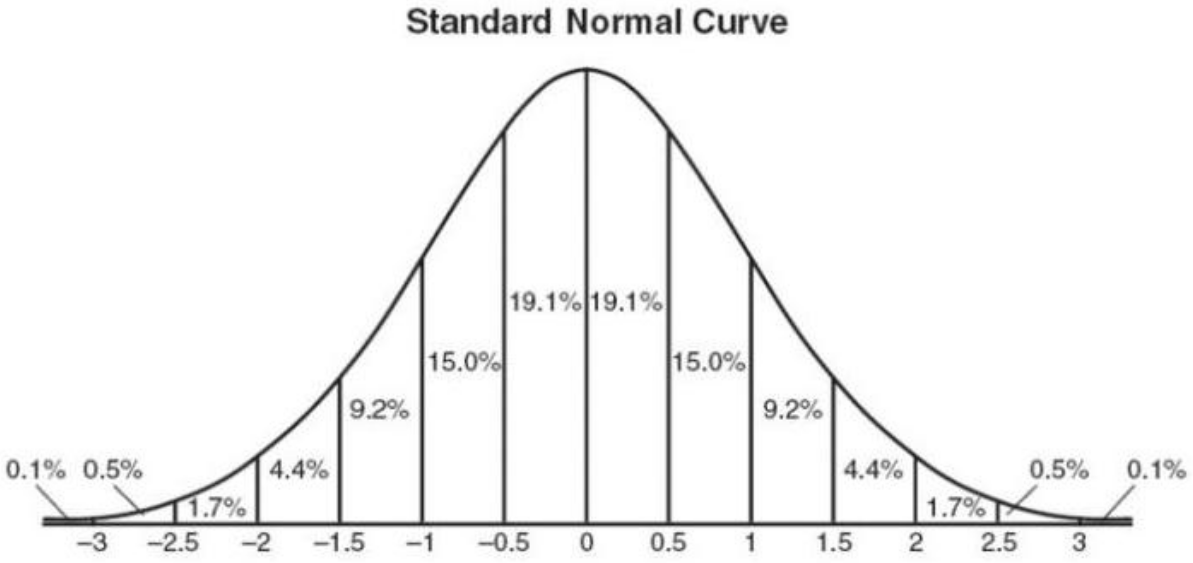
\includegraphics[scale=.3]{images/standard-normal-small}
  \end{center}
\end{example}

\begin{remark}
  When reviewing the key step in \cref{ex:clt-coin-flipping}, it is helpful to
  recall the standardization transformation defined in
  \cref{rmk:standardization}. The central limit theorem says that,
  approximately, $\overline{X}\sim \mathcal{N}(\mu, \sigma^{2}/n)$. Hence, by
  \cref{rmk:standardization},
  \begin{equation*}
    \frac{\overline{X}-\mu}{\sigma/\sqrt{n}}\approx Z
  \end{equation*}
  where $Z\sim \mathcal{N}(0,1)$. This is what justifies the key step in
  \cref{ex:clt-coin-flipping}.
\end{remark}

\subsection{Point estimation}
\textit{Section 6.1}

Recall a \textbf{population} is a large body of data that is the target of our
interest, and a \textbf{statistic} is any quantity whose value can be computed from a
sample.

Often, we have some quantity of interest, called a \demph{target parameter},
and we want a single ``best guess'' of some quantity of interest. When this is
the case, the we call a statistic an estimator:

\begin{definition}[Estimator]
  \label{def:estimator}
  An \demph{estimator} is a statistic, that is a function
  $T(X_{1},\ldots,X_{n})$ of a sample, that is used to approximate a target
  parameter.
  An \demph{estimate} is the realized value of an
  estimator (e.g., a number) that is obtained when the sample is actually
  taken.
\end{definition}
In words, an estimator is a rule, often expressed as a formula, that tells us
how to calculate the value of an estimate based on the measurements contained
in a sample.

\newpage
\section{2026-04-08 | Week 12 | Lecture 26}

\subsection{Point estimation}
\textit{Chapter 6.1}



Recall a \textbf{population} is a large body of data that is the target of our
interest, and a \textbf{statistic} is any quantity whose value can be computed from a
sample.

Often, we have some quantity of interest, called a \demph{target parameter},
and we want a single ``best guess'' of some quantity of interest. When this is
the case, the we call a statistic an estimator:

\begin{definition}[Estimator]
  \label{def:estimator}
  An \demph{estimator} is a statistic, that is a function
  $T(X_{1},\ldots,X_{n})$ of a sample, that is used to approximate a target
  parameter.
  An \demph{estimate} is the realized value of an
  estimator (e.g., a number) that is obtained when the sample is actually
  taken.
\end{definition}
In words, an estimator is a rule, often expressed as a formula, that tells us
how to calculate the value of an estimate based on the measurements contained
in a sample.

\begin{example}[Broccoli Poll]
  \label{ex:broccoli-poll}
  Suppose the fraction of people in Hawaii who like broccoli is $p$. This is
  an unknown \textbf{target parameter}. We don't know what $p$ is, but we
  would like to estimate it.In principle, we could ask everyone in the state,
  but that would be impractical. Instead, we take a random sample: we choose
  randomly $n$ individuals and ask each of them whether they like broccoli or
  not. Let
  \begin{equation*}
    \widehat{p} := \text{ fraction of our sample who like broccoli}
  \end{equation*}
  Suppose we sample $n=100$ individuals and $20$ of them like broccoli. Then
  \begin{equation*}
    \widehat{p} = \frac{20}{100}=.2
  \end{equation*}

  The \textbf{sample} in this example consists of $n$ random variables
  $X_{1},\ldots,X_{n}$, where
  \begin{equation*}
    X_{i}  =\left\{ \begin{array}{l@{\quad:\quad}l} 1 & \text{i-th sampled person
          likes broccoli}\\ 0 &\text{they don't} \end{array}\right.
  \end{equation*}
  Our \textbf{point estimate} is $\widehat{p}=0.2$ and the \textbf{point
    estimator} is the function $\widehat{p} = \frac{X_{1}+\ldots+X_{n}}{n}$,
  which is a \textbf{sample mean}.

  Taking a step back, we can think of our estimate as
  \begin{equation*}
    \widehat{p} = p + \text{error of estimation}
  \end{equation*}
  It is perhaps clear that if we increase the sample size $n$, then the
  estimation error should decrease, so that
  \begin{equation*}
    \widehat{p} \to p \text{ as } n \to  \infty.
  \end{equation*}
\end{example}
\begin{definition}[Bias and standard error]
  \label{def:bias-and-standard-error}
  Let $\widehat{\theta}$ be a point estimator of a target parameter $\theta$.
  The \demph{bias} of $\widehat{\theta}$ is the number
  $\text{Bias}(\widehat{\theta})=\E[\widehat{\theta}]-\theta$. If
  $\text{Bias}(\widehat{\theta})=0$, we say that $\widehat{\theta}$ is
  \demph{unbiased}, otherwise we say it is \demph{biased}.

  The \demph{standard error} of $\widehat{\theta}$, denoted
  $\sigma_{\widehat{\theta}}$, is its standard deviation:
  \begin{equation*}
    \sigma_{\widehat{\theta}} = \sqrt{\Var(\widehat{\theta})}
  \end{equation*}
\end{definition}

\begin{example}[Broccoli poll continued]
  \label{ex:broccoli-poll-continued}
  In the broccoli example, the estimator we used was the \demph{sample mean:}
  \begin{equation*}
    \widehat{p} = \frac{X_{1}+\ldots+X_{n}}{n}.
  \end{equation*}
  \begin{claim}
    $\widehat{p}$ is unbiased.
  \end{claim}
  \begin{claimproof}
    \begin{align*}
      \E\left[\widehat{p} \right] 
      &= \E\left[\frac{X_{1}+\ldots+X_{n}}{n} \right] \\
      &= \frac{1}{n}\left( \E\left[X_{1} \right]+\ldots+ \E\left[X_{n} \right] \right) \\
      &= \frac{1}{n}(np) \\
      &= p.
    \end{align*}
  \end{claimproof}
  \begin{claim}
    $\sigma_{\widehat{p}}= \sqrt{\frac{p(1-p)}{n}}$.
  \end{claim}
  \begin{claimproof}
    First observe that for every $i\in \left\{1,\ldots,n\right\}$, we have
    \begin{equation*}
      \Var(X_{i}) = \E\left[X_{i}^{2} \right]- \left( \E\left[X_{i} \right] \right)^{2}= p-p^{2}=  p(1-p).
    \end{equation*}
    Using \cref{thm:variance-properties},
    \begin{align*}
      \Var(\widehat{p}) 
      &= \Var\left(\frac{X_{1}+\ldots+X_{n}}{n}  \right)\\
      &= \frac{1}{n^{2}}\left( \Var(X_{1}+\ldots+X_{n}) \right)\\
      &= \frac{1}{n^{2}}\left( \Var(X_{1})+\ldots+\Var(X_{n}) \right)
      &&\text{by independence}\\ 
      &=\frac{1}{n^{2}}\left( np(1-p) \right)\\ 
      &=\frac{p(1-p)}{n}
    \end{align*}
    Taking square roots implies the statement of the claim.
  \end{claimproof}


  Finally, since $\widehat{p}$ is a sample mean, the central limit theorem
  implies that its distribution is approximately normal:

  \begin{center}
    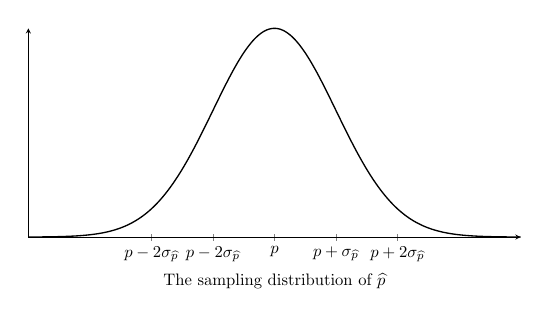
\begin{tikzpicture}[scale=.6]
      \begin{axis}[
        domain=0.44:0.68,
        samples=300,
        no markers,
        axis lines=left,
        xlabel={The sampling distribution of $\widehat{p}$},
        ylabel={},
        ymin=0,
        enlargelimits=false,
        width=12cm,
        height=6cm,
        xtick={0.5,.53,0.56,.59,0.62},
        xticklabels={$p-2\sigma_{\widehat{p}}$, $p-2\sigma_{\widehat{p}}$
          ,$p$, $p+\sigma_{\widehat{p}}$, $p+2\sigma_{\widehat{p}}$},
        ytick=\empty,
        clip=false
        ]
        % Normal pdf: mean=0.56, sd=0.03
        \addplot[thick]
        {1/(0.03*sqrt(2*pi))*exp(-((x-0.56)^2)/(2*(0.03)^2))};
       \end{axis}
    \end{tikzpicture}
  \end{center}
  As $n$ grows, the value of $\sigma_{\widehat{p}}=\sqrt{\frac{p(1-p)}{n}}$
  gets smaller, so the above curve (which is centered around the true
  parameter value $p$) gets narrower. 
\end{example}



\begin{example}[Estimating the sides of a dice]
  \label{ex:estimating-sides-dice}
  Suppose I roll a dice behind a screen, shouting out the number rolled each
  time. Your job is to estimate the number of sides of the dice, which we will
  call $\theta$.

  Given $n$ rolls, the sample consists of the $n$ random variables
  \begin{equation*}
    X_{1},\ldots,X_{n}
  \end{equation*}
  where $X_{i}$ is the $i^{\rm th}$ dice roll. We'll give two examples of
  estimators:

  \begin{itemize}
    \item Our first example is called the \textit{running maximum}, and it is
    defined as
    \begin{equation*}
      \widehat{\theta} = \max(X_{1},\ldots,X_{n}).
    \end{equation*}
    For example, if I roll the dice four times and obtain $3,11,7,$ and $4$,
    then your estimate would be that the dice has 11 sides.

    This sounds silly, but with enough data this estimator will give you the
    correct answer with high probability. This is because, if I roll the dice
    enough times, then I will eventually roll the highest number; hence,
    \begin{equation*}
      \lim_{n \to \infty} \widehat{\theta}(X_{1},\ldots,X_{n}) = \theta.
    \end{equation*}
    One drawback is that this estimator is biased because
    $\E[\widehat{\theta} ]<\theta$. This is because the estimator will
    ``usually'' be less than the true number of sides, and will never be
    more---so on average, $\widehat{\theta}$ will be smaller than $\theta$.
    
    \item Our second example is what is called the \textit{method of moments
      estimator}. In this setting, it's defined as
    \begin{equation*}
      \widehat{\theta} = 2 \left( \frac{X_{1}+\ldots+X_{n}}{n} \right)-1. 
    \end{equation*}

    Let's demystify this formula. Suppose $X$ a random variable representing
    one roll of the dice. We know that since the dice has $\theta$ sides, $X$
    has expected value
    \begin{equation*}
      \E\left[X \right] = \frac{1}{\theta}\left( 1+2+\ldots+\theta \right)  = \frac{\theta+1}{2}.
    \end{equation*}
    Rearranging, we get
    \begin{equation}\label{eq:7}
      \theta = 2 \E\left[X \right] -1.
    \end{equation}
    We also know that by the law of large numbers,
    $\E\left[X \right] \approx \frac{X_{1}+\ldots+X_{n}}{n}.$ Combining this
    with \cref{eq:7} implies
    \begin{equation*}
      \theta 
      \approx 2 \left( \frac{X_{1}+\ldots+X_{n}}{n} \right)-1.
    \end{equation*}
    The right hand side is what we've chosen to be our $\widehat{\theta}$, and
    hopefuly this calculation makes it seem like a reasonable choice.
    
    This estimator is unbiased. To see why, observe that
    \begin{align*}
      \E[\widehat{\theta} ] 
      &= \E\left[ 2 \left( \frac{X_{1}+\ldots+X_{n}}{n} \right)-1  \right] \\
      &= 2\E\left[   \frac{X_{1}+\ldots+X_{n}}{n}   \right] -1\\
      &= 2 \E\left[X \right]-1 \\
      &= \theta &&\text{by \cref{eq:7}.}
    \end{align*}
    
    In our example, with dice rolls $3,11,7$, and $4$, our estimator
    $\widehat{\theta}$ returns the estimate
    \begin{equation*}
      2 \left( \frac{3+11+7+4}{4} \right) -1 = 2 \left( \frac{25}{4} \right) -1 = 11.5.
    \end{equation*}
    So your estimate would be that the dice has 11.5 sides.
  \end{itemize}
\end{example}

Given two unbiased estimators, then \textit{ceteris paribus}, we would
typically prefer the estimator which has lower variance.
\newpage

\section{2026-04-13 | Week 13 | Lecture 27}

% With about 95\% probability, a normal random variable will lie within 2
% standard devations of its mean:
% \begin{center}
%   \begin{tikzpicture}[scale=.8]
%     \begin{axis}[
%       domain=0.44:0.68,
%       samples=300,
%       no markers,
%       axis lines=left,
%       xlabel={The sampling distribution of $\widehat{p}$},
%       ylabel={},
%       ymin=0,
%       enlargelimits=false,
%       width=12cm,
%       height=6cm,
%       xtick={0.5,0.56,0.62},
%       xticklabels={$p-2\sigma_{\widehat{p}}$,$p$,$p+2\sigma_{\widehat{p}}$},
%       ytick=\empty,
%       clip=false
%       ]
%       % Normal pdf: mean=0.56, sd=0.03
%       \addplot[thick]
%       {1/(0.03*sqrt(2*pi))*exp(-((x-0.56)^2)/(2*(0.03)^2))};

%       % Shaded region between 0.50 and 0.62
%       \addplot[
%       draw=none,
%       fill=gray,
%       fill opacity=0.35,
%       domain=0.50:0.62
%       ]
%       {1/(0.03*sqrt(2*pi))*exp(-((x-0.56)^2)/(2*(0.03)^2))}
%       \closedcycle;

%       % Label in the middle of the shaded region
%       \node at (axis cs:0.56,6) {$95\%$};
      
%       % Optional vertical dashed guides at the bounds
%       \addplot[dashed] coordinates {(0.50,0) (0.50, {1/(0.03*sqrt(2*pi))*exp(-((0.50-0.56)^2)/(2*(0.03)^2))})};
%       \addplot[dashed] coordinates {(0.62,0) (0.62, {1/(0.03*sqrt(2*pi))*exp(-((0.62-0.56)^2)/(2*(0.03)^2))})};
%     \end{axis}
%   \end{tikzpicture}
% \end{center}
% For our broccoli example, we don't know the true value of
% $\sigma_{\widehat{p}}$, since $\sigma_{\widehat{p}}=\sqrt{\frac{p(1-p)}{n}}$
% and $p$ is unknown. But we can approximate it, as follows: since
% $\widehat{p}=.2$ and $n=100$, we have
% \begin{equation*}
%   \Var(\widehat{p}) = \sqrt{\frac{p(1-p)}{n}} \approx \sqrt{\frac{\widehat{p}(1-\widehat{p})}{n}}=\sqrt{\frac{.2(1-.2)}{100}} = .04
% \end{equation*}

% So the above shaded picture tells us that $\P\left[\left| p-\widehat{p}
%   \right| \leq .08\right]=.95$. Since $\widehat{p}=.2$, w

\subsection{Confidence intervals}
\textit{Section 7.1}


\begin{definition}[Confidence Interval]
  An interval $(\widehat{p}-\epsilon,\widehat{p}+\epsilon)$ is called
  \demph{95\% confidence interval} for the unknown parameter $p$ if
  $\epsilon>0$ is chosen large enough that
  \begin{equation}\label{eq:19}
    \P\left[\left| \widehat{p}-p \right| <\epsilon\right] \geq .95
  \end{equation}
\end{definition}
In words, the interval contains the true parameter with probability at least
$.95$.
\begin{example}
  Can we come up with a 95\% confidence interval for our broccoli poll? We
  already have $\widehat{p}=.2$. But we don't yet know how big $\epsilon$ needs
  to be. (Of course we want to pick the smallest $\epsilon$ possible, as that
  would give us a more informative confidence interval). To figure out how big 
  $\epsilon$ must be, we'll have to use the central limit theorem again.

  Formally, let
  \begin{equation*}
    \widehat{p}=\frac{X_{1}+\ldots+X_{n}}{n}
  \end{equation*}
  where
  \begin{equation*}
    X_{i}  =\left\{ \begin{array}{l@{\quad:\quad}l} 1 & \text{i-th sampled person
          likes broccoli}\\ 0 &\text{they don't} \end{array}\right.
  \end{equation*}
  By the central limit theorem,
  \begin{equation}\label{eq:25}
    \widehat{p} \approx p + \frac{\sigma}{\sqrt{n}}Z
  \end{equation}
  where $Z\sim \mathcal{N}(0,1)$ and $\sigma =\sqrt{\Var(X_{i})}=\sqrt{p(1-p)}$. We also
  don't know what $\sigma$ is, since it depends on the unknown parameter
  $p$, but we can approximate it:
  \begin{equation}\label{eq:26}
    \sigma = \sqrt{\Var(X_{i})} = \sqrt{p(1-p)} \approx \sqrt{\widehat{p}(1-\widehat{p})=(.2)(.8)}=\sqrt{.16} = .4
  \end{equation}

  By \cref{eq:25},
  \begin{align*}
    \left| \widehat{p}-p \right| 
    &= \frac{\sigma}{\sqrt{n}}|Z|\\
    &= \frac{.4}{10} |Z|\\
    &= .04 |Z|
  \end{align*}

  Therefore
  \begin{align*} 
    \P\left[|\widehat{p}-p| \leq \epsilon\right] 
    &= \P\left[.04|Z| \leq\epsilon \right] \\
    &= \P\left[|Z| \leq 25\epsilon\right]\\
    &= \P\left[-25\epsilon \leq Z \leq 25 \epsilon\right]
  \end{align*}
  By the empirical rule, $\P\left[-2 \leq Z \leq 2\right]=.95$, so we need
  $25\epsilon=2$, or $\epsilon= .08$.

  Therefore the 95\% confidence interval is the interval
  \begin{equation*}
    (\widehat{p}-\epsilon, \widehat{p}+\epsilon) = (.12,.28).
  \end{equation*}

  We conclude that with $95\%$ confidence, the true proportion of people in
  Hawaii who like broccoli is between $12\%$ and $28\%$. Our point estimate is
  $0.2$, and our \demph{margin of error} is $0.08$.

  If we had sampled more people, our margin of error would be smaller. How many
  people would we have to sample to reduce the margin of error to $0.05$? What
  about to $0.01$?
\end{example}



\section{2026-04-15 | Week 13 | Lecture 28}
\subsection{The Coupon Collector Problem}

\begin{example}
  Joe is collecting coupons, numbered $1,\ldots,k$ . There are $n$ different
  coupons, and when he gets all $n$ of them, he gets a prize. Each time he
  gets a coupon, it is chosen uniformly at random (i.e., all coupons are
  equally likely).

  Find a value $m$ such that if Joe collects at least $m$ coupons, then his
  probability of winning the prize is at least $99\%$.

  \fl{Solution:} Let $m$ be any positive integer greater than $n$. Let
  \begin{equation*}
    V = \text{number of coupons Joe collects until he gets the prize}
  \end{equation*}
  and let
  \begin{equation*}
    A_{k} = \text{coupon $k$ is not collected in the first $m$ coupons}.
  \end{equation*}
  To solve the problem, want to find a value of $m$ sufficiently large that
  \begin{equation*}
    \P\left[V \leq m\right] \geq .99.
  \end{equation*}
  Equivalently, we want
  \begin{equation*}
    \P\left[V>m \right] \leq 0.01.
  \end{equation*}% If Joe collects at least $m$ coupons, he will get the prize with probability
  % at least $.99$.

  \begin{align*}
    \P\left[V>m \right] 
    &= \P\left[A_{1}\cup A_{2}\cup \ldots \cup A_{n} \right]\\
    &\leq \P\left[A_{1} \right]+ \P\left[A_{2} \right]+\ldots+\P\left[A_{n}
      \right] &&\text{(the union bound)}\\
    &\leq n \left( 1-\frac{1}{n} \right)^{m}\\ 
    &= n \left[ \left( 1-\frac{1}{n} \right)^{n}  \right]^{\frac{m}{n}}\\
    &\approx n \left[ e^{-1} \right]^{\frac{m}{n}}\\ 
    &= ne^{-m/n}
  \end{align*}
  Setting
  \begin{equation*}
    ne^{-m/n}<0.01
  \end{equation*}
  we can solve for $m$:
  \begin{equation*}
    e^{-m/n}< \frac{0.01}{n}
  \end{equation*}
  \begin{equation*}
    -\frac{m}{n} < \log \left( \frac{0.01}{n} \right) 
  \end{equation*}
  or
  \begin{equation*}
    m > - n\log\left(\frac{0.01}{n} \right) 
  \end{equation*}
  or equivalently,
  \begin{equation*}
    m > n \log\left(100n \right) 
  \end{equation*}
  In other words, if Joe collects at least $n \log\left(100n \right)$ coupons,
  then with probability at least $99\%$, he will get the prize.

  For example, if $n=15$, then $15\log(100\cdot15)=109.7$ so $m=110$ coupons is
  sufficient to ensure that Joe has 99\% probability of getting the prize.
\end{example}



\subsection{Hypothesis Testing}
\textit{Textbook section 8.1}

\fl{The hypothesis testing framework:} suppose you observe some random
quantity, which is assumed to depend on some unknown numerical parameter
$\theta$. You make a \textit{hypothesis}, which can be any claim about the
value of some parameter.

We are interested in testing the following two hypotheses:
\begin{itemize}
  \item The \demph{null hypothesis:} whatever effect you observed was
  due to random chance. This is denoted $H_{0}$.
  \item The \demph{alternative hypothesis:} the claim you made about the
  parameter. This is usually denoted $H_{a}$ 
\end{itemize}

Based on our observation(s) we will make a decision to either reject $H_{0}$,
or fail to reject $H_{0}$. 

Suppose the observed data is $X$. The \demph{p-value} of $X$ is defined as
\begin{equation*}
  \text{p-value} := \P\left[\text{observing a result at least as extreme as }X
    \text{ when }H_{0} \text{ is true} \right]
\end{equation*}
When the $p$-value is small, we \textbf{reject $H_{0}$}.

In particular, we set a \demph{significance level}, denoted $\alpha$, as the
cutoff such that we reject $H_{0}$ is $p<\alpha$ and we fail to reject $H_{0}$ if
$p \geq \alpha$.


A typical value is $\alpha=.05$ or $\alpha=.01$. 



This is the basic story. Let's do an example:



\begin{example}
  Suppose you have a coin but you don't know if it is a fair coin or not. You
  think maybe the coin is biased in favor of flipping heads. As an experiment,
  you flip the coin 10 times and you get 8 heads. Is this convincing evidence
  that the coin is biased?

  In this case, the data is an IID sample
  \begin{equation*}
    X_{1},\ldots,X_{10}
  \end{equation*}
  where
  \begin{equation*}
    X_{i}= \left\{ \begin{array}{l@{\quad:\quad}l} 1 & \text{with probability }\theta\\ 0&\text{with probability }1-\theta \end{array}\right.
  \end{equation*}
  The null hypothesis is
  \begin{equation*}
    H_{0}: \theta=\frac{1}{2}
  \end{equation*}
  The alternative hypothesis is that heads is more likely than tails:
  \begin{equation*}
    H_{1}: \theta>\frac{1}{2}
  \end{equation*}

  The p-value is
  \begin{align*}
    p 
    &= \P\left[\text{at least 8 heads when } \theta=\frac{1}{2} \right]\\
    &= {10 \choose 8}\theta^{8}(1-\theta)^{2}+{10 \choose
      9}\theta^{9}(1-\theta)^{1}+{10 \choose 10}\theta^{10}(1-\theta)^{0}
      \text{ with } \theta=\frac{1}{2}\\
    &= {10\choose 8} \left( \frac{1}{2} \right)^{10} +{10\choose 9} \left( \frac{1}{2} \right)^{10} +{10\choose 10} \left( \frac{1}{2} \right)^{10}\\ 
    &= \frac{7}{128}\\
    &\approx 0.0546.
  \end{align*}
  In words, if the coin were fair, we would expect it to flip 8 or more heads
  (out of ten) about 5\% of the time. That's not actually super rare, so while
  this is consistent with the coin being biased, it's also consistent with the
  null hypothesis. Hence, I wouldn't find this to be convincing evidence that
  the coin isn't fair, so I wouldn't reject the null hypothesis.

  Maybe you would. The cutoff for what is ``convincing'' is necessarily subjective.
\end{example}

\newpage
\section{2026-04-17 | Week 13 | Lecture 29}




\subsubsection{What is a hypothesis test?}
\begin{definition}[Hypothesis Testing]
  \label{def:hypothesis-testing}
  Given a sample from $X_{1},\ldots,X_{n}$ from a distribution depending on
  parameter $\theta$. We are interested in comparing two competingk
  hypotheses: a null hypothesis $H_{0}$ and an alternative hypothesis $H_{a}$.
  A \demph{hypothesis test} is a procedure or decision rule utilizing a
  statistic $T$ which specifies for which values of $T$ the hypothesis $H_{0}$
  is rejected, and for which values $H_{0}$ is accepted. The statistic $T$ is
  called the \demph{test statistic}.

  Associated with a hypothesis test is a \demph{rejection region} (RR), the set
  which specifies the values of the test statistic for which the null hypothesis
  to be rejected in favor of the alternative hypothesis. That is, if
  $T\in\mathrm{RR}$, then we reject $H_{0}$. If $T\notin \mathrm{\mathrm{RR}}$,
  we accept $H_{0}$.
\end{definition}


\begin{example}
  Suppose you have a coin but you don't know if it is a fair coin or not. You
  think maybe the coin is biased in favor of flipping heads. As an experiment,
  you flip the coin 10 times and you get 8 heads. Is this convincing evidence
  that the coin is biased?

  In this case, the data is an IID sample
  \begin{equation*}
    X_{1},\ldots,X_{10}
  \end{equation*}
  where
  \begin{equation*}
    X_{i}= \left\{ \begin{array}{l@{\quad:\quad}l} 1 & \text{with probability }\theta\\ 0&\text{with probability }1-\theta \end{array}\right.
  \end{equation*}
  The null hypothesis is
  \begin{equation*}
    H_{0}: \theta=\frac{1}{2}
  \end{equation*}
  The alternative hypothesis is that heads is more likely than tails:
  \begin{equation*}
    H_{1}: \theta>\frac{1}{2}
  \end{equation*}

  The p-value is
  \begin{align*}
    p 
    &= \P\left[\text{at least 8 heads when } \theta=\frac{1}{2} \right]\\
    &= {10 \choose 8}\theta^{8}(1-\theta)^{2}+{10 \choose
      9}\theta^{9}(1-\theta)^{1}+{10 \choose 10}\theta^{10}(1-\theta)^{0}
      \text{ with } \theta=\frac{1}{2}\\
    &= {10\choose 8} \left( \frac{1}{2} \right)^{10} +{10\choose 9} \left( \frac{1}{2} \right)^{10} +{10\choose 10} \left( \frac{1}{2} \right)^{10}\\ 
    &= \frac{7}{128}\\
    &\approx 0.0546.
  \end{align*}
  In words, if the coin were fair, we would expect it to flip 8 or more heads
  (out of ten) about 5.46\% of the time.

  
  In the previous example, the test statistic was
  $T=\text{(number of heads)}$. A reasonable rejection region might be
  $\left[ T \geq 8\right]$ or $\left[ T \geq 9\right]$.
\end{example}

\begin{example}
  Now, suppose that we flip the coin 100 times and we get 80 of them to be
  heads. Is this convincing evidence that the coin isn't fair?

  To answer this question, we'll compute the $p$-value. Let
  $X_{1},\ldots,X_{100}$ be our IID random sample, where
  \begin{equation*}
    X_{i} = \left\{ \begin{array}{l@{\quad:\quad}l}
        1 & \text{if $i$th coin is heads}\\
        0& \text{otherwise} \end{array}\right.
  \end{equation*}
  Then the number of heads is the random variable
  \begin{equation*}
    S_{n} = X_{1}+\ldots+X_{n}.
  \end{equation*}
  Observe that $\mu= \E\left[X_{i} \right]= \frac{1}{2}$ and $ $ Assuming the
  coin is a fair coin, we have
  \begin{equation*}
    \mu = \E\left[X_{i} \right] = \frac{1}{2}
  \end{equation*}
  and
  \begin{equation*}
    \sigma^{2} = \E\left[X_{i}^{2} \right] - \frac{1}{4} = \frac{1}{2}-\frac{1}{4} = \frac{1}{4}
  \end{equation*}
  so that
  \begin{equation*}
    \sigma= \frac{1}{2}.
  \end{equation*}
  By the central limit theorem, we know that
  \begin{align*}
    \frac{S_{n}}{n} \approx \mu + \frac{\sigma}{\sqrt{n}}Z, 
  \end{align*}
  where $Z$ is a standard normal random variable. For this specific problem,
  we have:
  \begin{equation*}
    \frac{S_{100}}{100} \approx \frac{1}{2}+\frac{1}{20}Z.
  \end{equation*}
  We can now compute the $p$-value:
  \begin{align*}
    \text{p-value }
    &= \P\left[\text{at least 80 heads out of 100 tosses}\mid \text{coin is fair} \right]\\
    &= \P\left[S_{100}\geq 80 \mid \text{coin is fair}\right]\\
    &= \P\left[\frac{S_{100}}{100}\geq .8 \mid \text{coin is fair}\right]\\
    &\approx \P\left[\frac{1}{2}+\frac{Z}{20} \geq .8\right] &&\text{Key
                                                                step. Follows by CLT.}\\
    &= \P\left[\frac{Z}{20} \geq .3\right]\\
    &= \P\left[Z \geq 6 \right]\\
    &\approx .000000001
  \end{align*}
  In other words, if the coin were a fair coin, observing heads at least 80 out of 100
  times would be extraordinarily unlikely. Therefore we reject $H_{0}$. 
\end{example}


\subsubsection{Type I and Type II errors}
There are two types of decision errors in the hypothesis testing framework.

\begin{definition}[Decision errors]
  \label{def:decision-errors}
  A \demph{type I error} is made if $H_{0}$ is rejected when $H_{0}$ is true.
  The probability of a type I error is denoted by $\alpha$:
  \begin{equation*}
    \alpha = \Pr \left[ \text{Type I error} \right] = \Pr\left[
      \text{rejecting $H_{0}$ when $H_{0}$ is true}\right]
    %%% T\in \text{RR} \mid H_{0} \text{ is true}\right].
  \end{equation*}
  The value of $\alpha$ is called the \demph{significance level} (or just
  \demph{level}) of the test.

  Similarly, a
  \demph{type II error} is made if $H_{0}$ is accepted when $H_{a}$ is true.
  We denote the probability of this happening by $\beta$:
  \begin{equation*}
    \beta = \Pr \left[ \text{Type II error} \right] = \Pr \left[
      \text{accepting $H_{0}$ when $H_{a}$ is true} \right] 
    % \P\left[ T\notin \text{RR} \mid H_{a} \text{ is true}\right].
  \end{equation*}
  The value $1-\beta$ is called the \demph{power} of the test.
\end{definition}

These types of errors, and their probabilities, can be summarized in the
following table:

\begin{center}
  \begin{tabular}{lcc}
    & Reject $H_0$ & Accept $H_0$ \\ \cline{2-3}
    \multicolumn{1}{l|}{$H_0$ true}
    & \multicolumn{1}{l|}{\makecell[c]{Type I error \\ $\text{level}=\alpha$}}
    & \multicolumn{1}{l|}{\makecell[c]{Correctly accept $H_{0}$ \\ $1-\alpha$}} \\ \cline{2-3}
    \multicolumn{1}{l|}{$H_a$ true}
    & \multicolumn{1}{l|}{\makecell[c]{Correctly reject $H_{0}$ \\ $\text{power}=1-\beta$}}
    & \multicolumn{1}{l|}{\makecell[c]{Type II error \\ $\beta$}} \\ \cline{2-3}
  \end{tabular}
\end{center}


\newpage
\section{2026-04-20 | Week 14 | Lecture 30}

\subsection{Decision errors}

\begin{example}[Coin flipping hypothesis test]
  \label{ex:coin-flipping-hypothesis-test}
  Flip a coin 10 times. Let $p$ be the probability of heads. Consider the
  hypothesis testing problem
  \begin{equation*}
    H_{0}: p = \frac{1}{2} \quad \text{versus} \quad H_{a}: p\neq \frac{1}{2}.
  \end{equation*}
  Let our test statistic be
  \begin{equation*}
    T = \text{(\# of heads)}
  \end{equation*}
  So $T$ takes a value between 0 and 10. If $H_{0}$ were true, then (one can
  check that) there would be about 97.9\% chance of getting between 2 and 8
  heads. So it might be reasonable to define our rejection region to be the
  set
  \begin{equation*}
    \text{RR} = \left\{0,1,9,10\right\}
  \end{equation*}
  since it is improbable to get these values with a fair coin. Using this
  rejection region, if $T=0,1,9$ or $10$, we would reject $H_{0}$ and conclude
  the coin is not a fair coin.

  This test is not perfect: assuming that $H_{0}$ is true, we will nonetheless
  reject $H_{0}$ about $2.1\%$ of the time.
\end{example}


\subsubsection{Type I and Type II errors}
There are two types of decision errors in the hypothesis testing framework.

\begin{center}
  \begin{tabular}{lcc}
    & Reject $H_0$ & Accept $H_0$ \\ \cline{2-3}
    \multicolumn{1}{l|}{$H_0$ true}
    & \multicolumn{1}{l|}{\makecell[c]{Type I error \\ $\text{level}= \P\left[\text{type I error} \right]=\alpha$}}
    & \multicolumn{1}{l|}{\makecell[c]{Correctly accept $H_{0}$ \\ $1-\alpha$}} \\ \cline{2-3}
    \multicolumn{1}{l|}{$H_a$ true}
    & \multicolumn{1}{l|}{\makecell[c]{Correctly reject $H_{0}$ \\ $\text{power}=1-\beta$}}
    & \multicolumn{1}{l|}{\makecell[c]{Type II error \\ $\P\left[\text{type II error} \right]=\beta$}} \\ \cline{2-3}
  \end{tabular}
\end{center}


% \begin{table}[H]
%   \centering
%   \begin{tabular}{lll}
%     & Reject $H_0$                      & Accept $H_0$                       \\ \cline{2-3} 
%     \multicolumn{1}{l|}{$H_0$ true} & \multicolumn{1}{l|}{Type-I Error \\ $\alpha$ } & \multicolumn{1}{l|}{Correct \\ $1-\alpha $ }       \\ \cline{2-3} 
%     \multicolumn{1}{l|}{$H_1$ true} & \multicolumn{1}{l|}{Correct\\ $1-\beta$ }      & \multicolumn{1}{l|}{Type-II Error $\beta$ } \\ \cline{2-3} 
%   \end{tabular}
% \end{table}


\begin{example}[\cref{ex:coin-flipping-hypothesis-test} continued]
  In \cref{ex:coin-flipping-hypothesis-test}, the level of the test is
  $\alpha=2.1\%$. Note that $\beta$ is a function of $p$. For example if
  $p=0.4$, then
  \begin{align*}
    \beta 
    &=\beta(0.4)\\
    &= \P\left[\text{Type II error}\mid p=0.4 \right]\\
    &= \P\left[T\notin \text{RR} \mid p=0.4  \right]\\
    &= \sum_{k=2}^{8} {10\choose k}(0.4)^{k}(1-0.4)^{10-k}\\
    &=.952
  \end{align*}
  Therefore if the true value of $p$ is $.4$, then the power of the the test
  is $.048$.

  On the other hand if the true value of $p$ is $p=.1$, then $\beta(.1)=.264$,
  so the power of the test would be $.736$. We generally don't know what the
  true power of the test is, since that would require knowing the value of the
  parameter (in which case we wouldn't be doing a hypothesis test...).

  It is a common mistake to assume that $\alpha+\beta=1$. In general,
  $\alpha+\beta\neq 1$. 
\end{example}


These terms are clarified by an example.

\begin{remark}[Decision Errors]
  \label{rmk:decision-errors}
  A Ukrainian drone operator spots an unmarked vehicle traveling down a road.
  She needs to make a decision about whether to strike the truck. The
  hypothesis test is the following:
  \begin{align*}
    H_{0}:& \text{ the target is not a Russian military vehicle}\\
    H_{a}:& \text{ the target is a Russian military vehicle}
  \end{align*}
  Rejecting $H_{0}$ means giving an order to destroy the target. Accepting
  $H_{0}$ means `take no action'.

  In this context, a Type-I error occurs when the operator gives the order to
  destroy the vehicle, but it turns out the vehicle is not Russian military. A
  Type-II error, on the other hand, has occurred if she doesn't order the
  strike, but the vehicle really was a Russian military vehicle.
  \begin{itemize}
    \item A Type-I error means she killed a civilian or a friendly unit (an
    error of commission).
    \item A Type-II error means she missed an opportunity to kill an enemy (an
    error of ommission).
  \end{itemize}
  Here, the terms ``power'' and ``level'' have the following meaning:
  \begin{itemize}
    \item The \textbf{power} of the test is the probability that she
    orders a strike when a Russian military vehicle goes by. (She wants this
    to be high).
    \item The \textbf{level} of the test is the probability that she orders a
    strike when a civilian goes by. (She wants this to be low).
  \end{itemize}
  Ideally, the operator would like to eliminate both types of errors
  (accidentally killing civilians vs failing to kill enemy). That is, she
  would like
  \begin{equation*}
    \alpha=\Pr\left[\text{Type I error} \right]= 0 \quad \text{and} \quad
    \beta=\Pr\left[\text{Type II error} \right]=0.
  \end{equation*}
  Unfortunately, it is impossible to simultaneously eliminate both types of
  error without perfect information. On one hand, the drone operatore could
  minimize the probability of a type I error by simply never ordering a strike,
  in which case $\alpha= \Pr\left[ \text{Type I error} \right] = 0$. But this
  is unsatisfactory, since in that case,
  $\beta= \Pr\left[\text{Type II error} \right]=1$. On the other hand, she
  could maximize the power by simply always ordering a strike; in that case,
  $\beta=0$ but $\alpha=1$. This tradeoff is present in every hypothesis test.
  
  The approach that the hypothesis testing framework takes to address this
  tradeoff is to (1) set a maximal level $\alpha$ that one is willing to
  accept, and then (2) find the most powerful test subject to that constraint.

  Of course, the appropriate significance level to set depends on the
  situation: a truck speeding towards the operator's position is very
  different from a truck traveling away from the front.
\end{remark}



% Therefore
% \begin{align*}
%   \P\left[\left| \widehat{p}-p \right| < \epsilon \right] 
%   &\approx \P\left[\frac{\sigma}{\sqrt{n}}|Z| <\epsilon\right]\\
%   &= \P\left[|Z| <\frac{\epsilon \sqrt{n}}{\sigma}\right]\\
%   &\geq \P\left[|Z|<\frac{\epsilon \sqrt{n}}{1/2} \right] &&\text{(since $\sigma \leq 1/2$)}.\\
%   &= \P\left[|Z|<2\epsilon \sqrt{n} \right]\\
%   &=2\Phi(2\epsilon \sqrt{n}) -1
% \end{align*}

% In conclusion we have:
% \begin{empheq}[box=\boxmath]{equation}
%   \label{eq:confidence-intervals}
%   \P\left[\left| \widehat{p}-p \right| < \epsilon \right]  \geq 2\Phi(2\epsilon \sqrt{n}) -1
% \end{empheq}
% Thus in order for the left hand side to be greater than $.95$, it will suffice
% for
% \begin{equation*}
%   2\Phi(2\epsilon \sqrt{n}) -1 \geq 0.95
% \end{equation*}
% or equivalently
% \begin{equation*}
%   \Phi(2\epsilon \sqrt{n}) \geq 0.975.
% \end{equation*}
% Using a computer, we can determine that $\Phi(u) \geq 0.975$ whenever $u \geq
% 1.96$. Thus, we need
% \begin{equation*}
%   2\epsilon \sqrt{n} \geq 1.96.
% \end{equation*}
% For our problem, $n=100$, so $\sqrt{n}=10$, so we need $\epsilon$ to be at
% least as big as
% \begin{equation*}
%   \epsilon \geq 1.96/20 = 0.098.
% \end{equation*}
% Thus, our confidence interval is
% \begin{equation*}
%   (\widehat{p}-\epsilon,\widehat{p}+\epsilon) = (0.2-0.098, 0.2+0.098) = (.102, .298).
% \end{equation*}


\newpage


\section{2026-04-22 | Week 14 | Lecture 31}
\subsection{Tests of independence}
\textit{Based on chapters 14.2-14.4}

Suppose we want to know if two things $A$ and $B$ are related to each other,
or whether they are independent. For example, whether or not a person vapes
(A) and whether they get coronary artery disease (B).

Or: whether a student attends class regularly (A) and whether they pass the
class (B).

\Fl{Question:} How can we test this (using the hypothesis testing framework)?

\Fl{Answer:} We can utilize what are called ``tests of independence'', which
we'll present in this lecture. For such tests, we require two main ingredients.

\subsubsection{Ingedient 1: The chi-squared distribution}


\begin{definition}[Chi-Squared Distribution]
  \label{def:chi-squared-distribution}
  Let $k$ be a positive integer. A nonnegative random variable $X$ is said to
  have \demph{chi-squared distribution} with $d$ \demph{degrees of freedom} if
  it has pdf
  \begin{equation*}
    f(x) 
    = \left\{ 
      \begin{array}{l@{\quad:\quad}l} \frac{1}{2^{d/2}\Gamma(d/2)}x^{\frac{d}{2}-1}e^{-x/2} & x \geq 0\\ 0& x<0\end{array}\right.
  \end{equation*}.
\end{definition}

Here, $\Gamma(x)= \int_{0}^{\infty}t^{x-1}e^{-t}dx$. Note $\Gamma(k)=(k-1)!$
if $k$ is a positive integer.

From left-to-right, here's what $f(x)$ looks like for $d=2$, $d=4$, and
$d=12$:
\begin{center}
  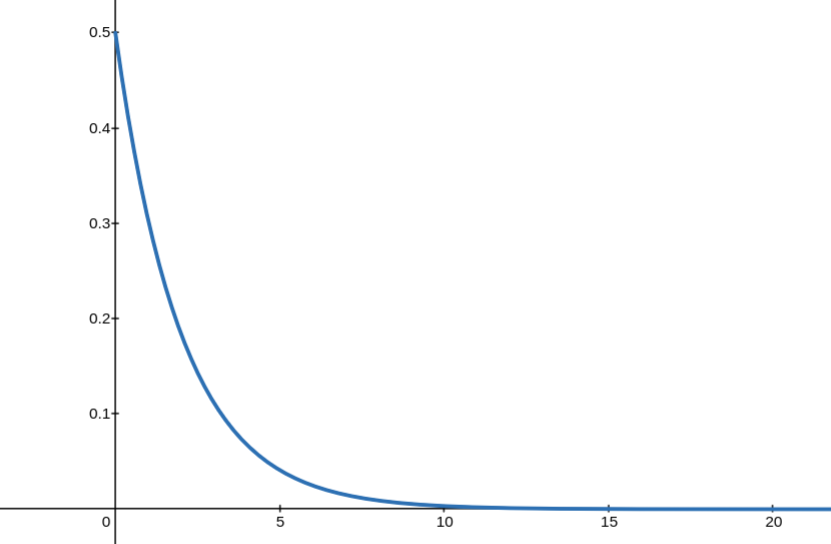
\includegraphics[scale=0.15]{images/chi-squared-d2}
  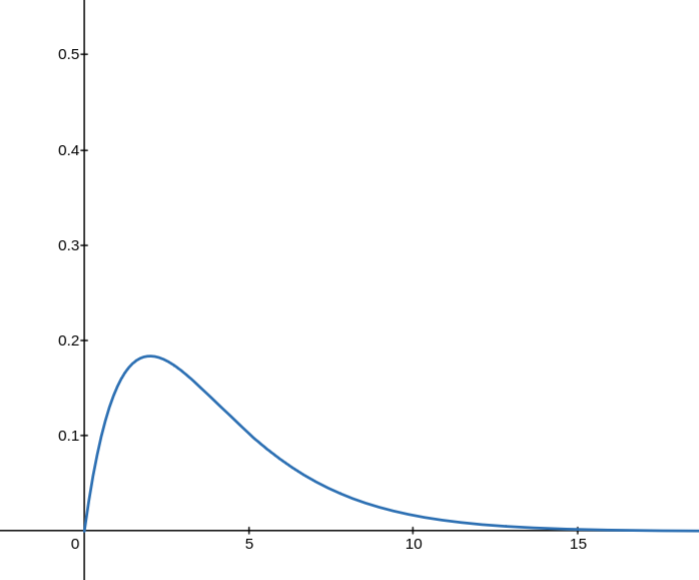
\includegraphics[scale=0.15]{images/chi-squared-d4}
  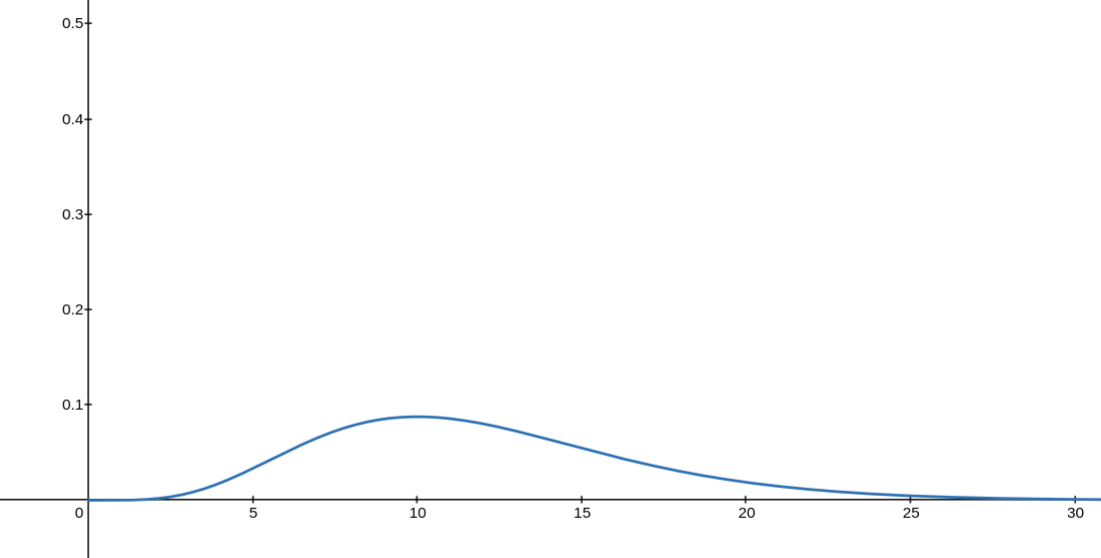
\includegraphics[scale=0.15]{images/chi-squared-d12}
\end{center}

\begin{proposition}
  A $\chi^{2}$ random variable $X$ with $d$ degrees of freedom has
  \begin{equation*}
    \E\left[X \right] = \alpha\beta = d \quad \text{and} \quad \Var(X) = \alpha\beta^{2} = 2d
  \end{equation*}
\end{proposition}

The chi-squared distribution plays a central role in statistical inference. It
is completely determined by its degrees of freedom.


\subsubsection{Ingedient 2: The chi-squared statistic}



\begin{definition}[Chi-squared statistic]
  
  Suppose we repeatedly conduct an experiment with $k$ possible outcomes. The
  \demph{chi-squared statistic} is defined as
  \begin{equation}\label{eq:29}
    \chi^{2}:= \sum_{i=1}^{k} \frac{\left(N_{i}-E_{i}\right)^{2}}{E_{i}},
  \end{equation}
  where $E_{i} = (\text{expected \# of times outcome $i$ occurs})$, and
  $N_{i}= (\text{\# of times outcome $i$ is observed})$.
\end{definition}

\begin{remark}
  The right-hand side of \cref{eq:29} has the form
  \begin{equation*}
    \sum_{i=1}^{k} \frac{\left( \text{observed}- \text{expected} \right)^{2} }{ \text{expected}} 
  \end{equation*}
\end{remark}



\begin{remark}
  \label{rem:chi-squared-theorem}
  Under general conditions, the chi-squared statistic $\chi^{2}$ has approximately a
  chi-squared distribution with degrees of freedom determined by the setting.
  % the 
  % \begin{equation*}
  %   \chi^{2} := \sum_{i=1}^{k} \frac{\left(X_{i}-np_{i}\right)^{2}}{np_{i}}.
  % \end{equation*}
  % Then $\chi^{2}$ has approximately chi-squared distribution with $k-1$ degrees of
  % freedom (as long as  $np_{i}\geq 5$ for all $i=1,\ldots,m$).
\end{remark}

% \begin{theorem}
%   \label{rem:chi-squared-theorem}
%   If $X=(X_{1},\ldots,X_{k})$ is a multinomial random variable with
%   parameters $p_{1},\ldots,p_{k}$, then 
%   \begin{equation*}
%     \chi^{2} = \sum_{i=1}^{k} \frac{\left(X_{i}-np_{i}\right)^{2}}{np_{i}}.
%   \end{equation*}
%   If $np_{i}\geq 5$ for all $i=1,\ldots,k$. Then $\chi^{2}$ has approximately
%   chi-squared distribution with $k-1$ degrees of freedom.
% \end{theorem}



% \begin{proof}[Proof sketch of \cref{rem:chi-squared-theorem}]
%   Key ingredients:
%   \begin{itemize}
%     \item By the central limit theorem, $\frac{X_{i}-np_{i}}{\sqrt{np_{i}}}$
%     is approximately normal.
%     \item So the chi-squared statistic is approximately a sum of squares of
%     independent standard normal random variables.
%     \item Which gives a chi-squared distribution by
%     \cref{thm:chi-squared-sum-squared-normals}.
%   \end{itemize}
%   The details of the proof rely on linear algebra.
% \end{proof}

\subsubsection{Example of a test of independence}
\begin{definition}
  A \demph{contingency table} is a matrix of with rows labeled as group 1,
  group 2, and so forth, and columns labeled as outcome 1, outcome 2, etc. The
  entries of the matrix are \textit{counts}: the $(i,j)$-th entry is the
  number of times that group $i$ experience outcome $j$.
\end{definition}

\begin{example}[Test of independence]
  For example, suppose we have a population of $n=54$ students, which we divide
  up according two to factors
  \begin{enumerate}[(i)]
    \item whether they attended class regularly or not
    \item whether they pass the class exam or not
  \end{enumerate}
  Then our contingency table is

  \begin{equation}\label{eq:table-of-observed-values}
    \begin{tabular}{l|cc}
      & \textbf{Pass} & \textbf{Fail} \\
      \hline
      \textbf{Attended} & 25          & 6            \\
      \textbf{Skipped}  & 8           & 15           
    \end{tabular} 
  \end{equation}
  This is the \demph{table of observed values}. We usually augment the table
  with ``marginal totals'', like so:


  \begin{center}
    \begin{tabular}{l|cc|c}
      & \textbf{Pass} & \textbf{Fail} & \textbf{Total} \\
      \hline
      \textbf{Attended} & 25 & 6  & 31 \\
      \textbf{Skipped}  & 8  & 15 & 23 \\
      \hline
      \textbf{Total}    & 33 & 21 & 54
    \end{tabular}
  \end{center}


  The null hypothesis is
  \begin{equation*}
    H_{0}= \text{ attendence and passing are independent}
  \end{equation*}
  and the alternative hypothesis is
  \begin{equation*}
    H_{a} = \text{ there is a relationship between attendence and passing.}
  \end{equation*}


  Let $p$ denote the probability that a student regularly attends class, and let
  $q$ denote the probability that a student passes the final exam.

  \fl{Important:} We do not know the true value of $p$ and $q$. But we can
  estimate them using the marginal row and column sums from the table:
  \begin{equation*}
    p \approx \frac{31}{54} \quad \text{and} \quad q\approx \frac{33}{54}
  \end{equation*}


  \Fl{Question:} What are the expected values of the table, assuming the null
  hypothesis is true?

  If attendence and passing are indpendent, then
  \begin{equation*}
    \E\left[\# \text{ of students who attend regularly AND pass} \right] = npq = (54)\left( \frac{31}{54} \right) \left( \frac{33}{54} \right)= 18.9
  \end{equation*}

  This is what we expect if the null hypothesis is true. Compare this with the
  actual observed value, which was $25$. The idea of the test, which we will
  finish in the next lecture, is the following:
  \begin{center}
    \textbf{If the observed values deviate a lot from what we'd expect under
    $H_{0}$, we should reject $H_{0}$.}
  \end{center}
  Quantifying this will require computing a chi-squared statistic, which we'll
  do in the next lecture.
\end{example}


\newpage
\section{2025-04-21 | Week 14 | Lecture 32}
\textit{Chapter 14.1 through 14.3}

We will finish the example of a test of independence from last time.

\begin{example}[Test of independence]
  For example, suppose we have a population of $n=54$ students, which we divide
  up according two to factors
  \begin{enumerate}[(i)]
    \item whether they attended class regularly or not
    \item whether they pass the class exam or not
  \end{enumerate}
  Then our contingency table is

  \begin{equation}\label{eq:table-of-observed-values}
    \begin{tabular}{l|cc}
      & \textbf{Pass} & \textbf{Fail} \\
      \hline
      \textbf{Attended} & 25          & 6            \\
      \textbf{Skipped}  & 8           & 15           
    \end{tabular} 
  \end{equation}
  This is the \demph{table of observed values}. We usually augment the table
  with ``marginal totals'', like so:

  \begin{center}
    \begin{tabular}{l|cc|c}
      & \textbf{Pass} & \textbf{Fail} & \textbf{Total} \\
      \hline
      \textbf{Attended} & 25 & 6  & 31 \\
      \textbf{Skipped}  & 8  & 15 & 23 \\
      \hline
      \textbf{Total}    & 33 & 21 & 54
    \end{tabular}
  \end{center}


  The null hypothesis is
  \begin{equation*}
    H_{0}= \text{ attendence and passing are independent}
  \end{equation*}
  and the alternative hypothesis is
  \begin{equation*}
    H_{a} = \text{ there is a relationship between attendence and passing.}
  \end{equation*}


  Let $p$ denote the probability that a student regularly attends class, and let
  $q$ denote the probability that a student passes the final exam.

  \fl{Important:} We do not know the true value of $p$ and $q$. But we can
  estimate them using the marginal row and column sums from the table:
  \begin{equation*}
    p \approx \frac{31}{54} \quad \text{and} \quad q\approx \frac{33}{54}
  \end{equation*}


  \Fl{Question:} What are the expected values of the table, assuming the null
  hypothesis is true?


  Under the null hypothesis, we can multiply probabilities, e.g., so that the
  probability that a student both regularly attends class AND passes the exam is
  about $pq$. Therefore, since there are $n$ students,
  \begin{align*}
    &\E\left[\text{\# of students who attend regularly AND pass the exam}\right] \\
    &= n \P\left[\text{a randomly-selected student attends regularly AND pass the exam} \right]\\
    &= n \P\left[\text{attends regularly}\right] \P\left[\text{passes the exam} \right]\\
    &= npq
  \end{align*}

  Similar calculations gives us the following table of expected counts:
  \begin{center}
    \begin{tabular}{l|cc}
      & \textbf{Pass} & \textbf{Fail} \\
      \hline
      \textbf{Attended} & $npq$          & $np(1-q)$            \\
      \textbf{Skipped}  & $n(1-p)q$           & $n(1-p)(1-q)$            
    \end{tabular}
  \end{center}
  and plugging in the values $n=54$ and our approximations
  $p\approx \frac{31}{54}$ and $q\approx \frac{33}{54}$ gives

  \begin{equation}\label{eq:table-of-estimated-expected-values}
    \begin{tabular}{l|cc}
      & \textbf{Pass} & \textbf{Fail} \\
      \hline
      \textbf{Attended} & $18.9$          & $12.1$            \\
      \textbf{Skipped}  & $14.1$           & $8.9$            
    \end{tabular}
  \end{equation}
  \textbf{Interpretation:} These are the values we would expect if $H_{0}$
  were true. If the observed values deviate too much from these values, that's
  evidence against the null hypothesis.
  
  Using the values recorded in Tables \ref{eq:table-of-observed-values} and
  \ref{eq:table-of-estimated-expected-values}, we can compute the chi-squared
  statistic:
  \begin{align*}
    \chi^{2} 
    &= \sum_{\text{all table entries}} \frac{\left( \text{observed
      value} - \text{expected value} \right)^{2} }{ \text{expected value}} \\
    &= \frac{\left( 25-18.9 \right)^{2} }{18.9}+ \frac{(6-12.1)^{2}}{12.1}+ \frac{\left( 8-14.1 \right)^{2} }{14.1}+ \frac{\left( 15-8.9 \right)^{2} }{8.9}\\
    &= 11.9
  \end{align*}

  By \cref{rem:chi-squared-theorem}, we know that $\chi^{2}$ has a chi-squared
  distribution. When computing a chi-squared test statistic from a contingency
  table for a test of independence, the degrees of freedom is given by the
  equation
  \begin{equation*}
    \text{df}=(\text{number of rows} -1)\times (\text{number of columns} -1)
  \end{equation*}
  which in our case, for a $2\times 2$ table, is just 1.

  Thereore, using \cref{def:chi-squared-distribution}, the p-value is
  \begin{align*}
    p \text{-value}
    &= \P\left[\chi^{2}\geq 11.9\right]\\
    &= \int_{11.9}^{\infty} \frac{1}{\sqrt{2\pi}} x^{-\frac{1}{2}}e^{-x/2}dx\\
    &=0.0006
  \end{align*}
  In other words, if attending and passing were independent, we would see
  results this extreme only 0.06\% of the time. This is very small, so we reject
  the null hypothesis. Our conclusion is that attendance and passing the final
  exam are \textbf{not independent}, i.e., that there is a relationship between
  them.

  At this point we are tempted to conclude that regularly attending class
  increases your chance of passing the final exam. This seems obvious and is
  certainly consistent with the data. But it's not a conclusion that follows
  from the test that we did. The test only told us that these two things things
  probably have some relationship; it doesn't give us information about the
  nature of that relationship.
\end{example}


\subsection{Interpreting tests of independence}

Suppose we want to know if two things $A$ and $B$ are related to each other.
We will discuss only the case where $A$ and $B$ are discrete, categorical
events. For example
\begin{equation*}
  A  = \left[ \text{a person vapes} \right] 
\end{equation*}
\begin{equation*}
  B = \left[ \text{person gets coronary artery disease (CAD)} \right] 
\end{equation*}
There are many possible relationships:


\begin{itemize}
  \item \textbf{Causality:} Vaping causes arterial disease.
  \begin{center}
    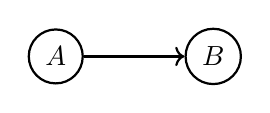
\begin{tikzpicture}[->, node distance=2cm, thick]
      \node[circle, draw] (A) {\(A\)}; \node[circle, draw, right of=A] (B)
      {\(B\)}; \draw (A) -- (B);
    \end{tikzpicture}
  \end{center}
  \item \textbf{Common Response:} Perhaps the effect of vaping on your
  arteries is perfectly benign (no causal relationship), but CAD and vaping
  are still positively associated due to the effect of some third variable $C$
  that causes both to occur simultaneously:
  \begin{center}
    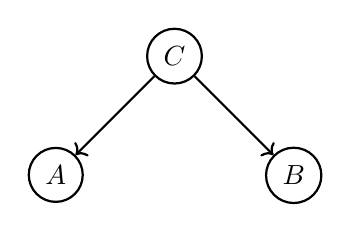
\begin{tikzpicture}[->, node distance=1cm and 1cm, thick]
      \node[circle, draw] (C) {\(C\)}; \node[circle, draw, below left=of C]
      (A) {\(A\)}; \node[circle, draw, below right=of C] (B) {\(B\)}; \draw
      (C) -- (A); \draw (C) -- (B);
    \end{tikzpicture}
  \end{center}
  For example we might have
  $C=\left[ \text{person smokes cigarettes} \right]$. Maybe vapers are
  disproportionately likly to have smoked cigarettes, and perhaps and it's
  this subset of vapers that drives the association between vaping and CAD, as
  cigarette smoking is well-established to cause CAD. If this is true, then
  quitting vaping woudn't decrease your chance of CAD.

  \item \textbf{Confounding:} (A third variable jointly influences or causes
  both $A$ and $B$). For example, suppose it were observed that vapers has
  have \textbf{lower} rates of coronary artery disease than the general
  population --- that doesn't mean vaping necessarily have a protective
  effect. For example, maybe the vapers are on average younger than the
  population (CAD usually develops in older people). In that case, we might
  observe a spurious relationship between $A$ and $B$ due to the effects of
  some other third variable, $C= \left[ \text{youth} \right]$:
  \begin{center}
    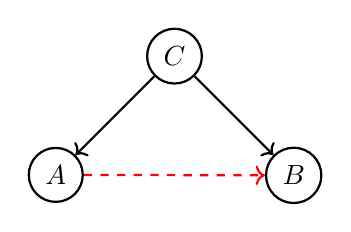
\begin{tikzpicture}[->, node distance=1cm and 1cm, thick]
      \node[circle, draw] (C) {\(C\)}; \node[circle, draw, below left=of C]
      (A) {\(A\)}; \node[circle, draw, below right=of C] (B) {\(B\)}; \draw
      (C) -- (A); \draw (C) -- (B); \draw[dashed, red] (A) --
      (B); % spurious association
    \end{tikzpicture}
  \end{center}
  It could nonetheless be the case that vaping increases your risk of CAD
  through some biological mechanism (the red dotted line), and due to the
  effect of age, vapers might \textit{still} have lower incidence of CAD than
  the general population.

  In order to rule this out, we'd need to \textit{control} for the effect of
  age, perhaps by conducting a study on people from the same age group.
\end{itemize}

What we \textit{can} say, however, is that if $A$ and $B$ do not have any
relationship (causal or otherwise), then they are probabilistically
independent. This is what tests of independence do. They ask the question
\textbf{``Are $A$ and $B$ independent?''} The answer to such tests is always
either ``no'' or ``maybe''. They don't give us much more information than
that.

\newpage
\section{2025-05-01 | Week 15 | Lecture 33}

\subsection{Simple linear regression (i.e., finding a best-fit line)}
\textit{Based on chapter 12.1 in the textbook}
\label{sec:finding-best-fit-line-with-linear-regression}
\begin{center}
  \begin{tcolorbox}[width=0.9\textwidth, colback=white, colframe=black]
    \textit{\textbf{The nexus question of this lecture:} How do we find the
      ``best fit'' line for data?}
  \end{tcolorbox}
\end{center}


Suppose we have four data points taking the form
$(t,b) = (\text{time}, \text{observation})$:
\begin{align*}
  (t_{1},b_{1}) &= (0,0)\\
  (t_{2},b_{2}) &= (1,8)\\
  (t_{3},b_{3}) &= (3,8)\\
  (t_{4},b_{4}) &= (4,20)
\end{align*}

I have plotted these below. The equation of a line is
\begin{equation*}
  y = C+Dt.
\end{equation*}
\begin{definition}
  The \demph{simple linear regression problem} is to find values for $C$ and $D$
  which best fit our data.
\end{definition}
Here's a picture of the data points and a general line $y=C+Dt$ which aims to
fit to the data:
\begin{center}
  \begin{tikzpicture}[x=3cm, y=.3cm]
    % axes
    \draw[->] (-.2,0) -- (4.3,0) node[right] {$t$}; \draw[->] (0,0) --
    (0,21.5) node[above] {$y$};

    % x-axis ticks and labels
    \foreach \x in {0,1,2,3,4} \draw (\x,.2) -- (\x,-0.2) node[below] {\x};

    % y-axis ticks and labels
    \foreach \y in {8,10,20} \draw (.02,\y) -- (-0.02,\y) node[left] {\y};

    % regression line y = 1 + 4x
    \draw[blue, dashed, thick] (-.2,.2) -- (4.1,17.4) node[right,blue] {$y=C+Dt$} ;

    % residuals (vertical segments)
    \draw[red,thick] (0,0) -- (0,1) node[pos=.5, right] {$e_1$};
    \draw[red,thick] (1,8) -- (1,5) node[pos=.5, right] {$e_2$};
    \draw[red,thick] (3,8) -- (3,13) node[pos=.5, right] {$e_3$};
    \draw[red,thick] (4,20) -- (4,17) node[pos=.5, right] {$e_4$};

    % points
    \fill (0,0) circle[radius=2pt]; \fill (1,8) circle[radius=2pt]
    node[above,right] {$(1,8)$}; \fill (3,8) circle[radius=2pt]
    node[above,right] {$(3,8)$}; \fill (4,20) circle[radius=2pt]
    node[above,right] {$(4,20)$};
  \end{tikzpicture}
\end{center}

Let $e_{i} = b_{i}-(C+Dt_{i})$ for each $i=1,\ldots,4$. In words, $e_{i}$ is
obtained by measuring the vertical distance between the line $y=C+Dt$ and the
$i^{\rm th}$ data point. For this example, we have
\begin{equation*}
  \mathbf{e} =
  \begin{bmatrix}
    e_{1}\\
    e_{2}\\
    e_{3}\\
    e_{4}
  \end{bmatrix}
  =
  \begin{bmatrix}
    0-C\\
    8-(C+D)\\
    8-(C+3D)\\
    20-(C+4D)
  \end{bmatrix}
\end{equation*}
This vector is called the \demph{residual vector}, and it consists of the
``errors'' between
\begin{enumerate}
  \item the observed data; and,
  \item the values predicted by the line $y=C+Dt$.
\end{enumerate}

% Its entries are found by
% computing the vector of vertical distances between the points and the line
% $y=C+Dt$, which are labelled in red on the above plot.

% The vector $\mathbf{e}$
% is known as the \demph{residual vector}, and the entries of $\mathbf{e}$ are
% known as the \demph{residuals}.

We want all four errors $e_{1},\ldots,e_{4}$ to be small. One way to measure
the total error is to square the four errors and add them up:
\begin{equation}\label{eq:12}
  \textrm{SSE} = e_{1}^{2}+e_{2}^{2}+e_{3}^{2}+e_{4}^{2}
\end{equation}
This is called the \demph{sum of squared errors} (SSE). Squaring has two
advantages: it makes all the errors positive, and it penalizes large errors.

Therefore, to find the best-fitting line $y=C+Dt$, our goal will be to find
values for $C$ and $D$ which minimize the sum of squared
errors $e_{1}^{2}+e_{2}^{2}+e_{3}^{2}+e_{4}^{2}$.


We'll present two approaches to finding the best values for $C$ and $D$.

\Fl{Approach \#1: Calculus}

Consider the function
\begin{align*}
  f(C,D) 
  &= e_{1}^{2}+e_{2}^{2}+e_{3}^{2}+e_{4}^{2} \\
  &= C^{2}+(8-C-D)^{2}+(8-C-3D)^{2}+(20-C-4D)^{2}.
\end{align*}
We can use calculus to minimize $f$. To find the critical point of $f$, we set
$\nabla f=0$ and solve for $C$ and $D$:
\begin{equation*}
  0\overset{set}{=}\frac{\partial f}{\partial C} = 2C-2(8-C-D)-2(8-C-3D)-2(20-C-4D) =-72+8C+16D
\end{equation*}
and
\begin{equation*}
  0\overset{set}{=}\frac{\partial f}{\partial D} = -2(8-C-D)-6(8-C-3D)-8(20-C-4D) = -224+16C+52D.
\end{equation*}
Combining these equations gives
\begin{equation*}
  \left\{ \begin{array}{l@{}l}  8C+16D = 72\\16C+52D=224  \end{array}\right..
\end{equation*}
After dividing both equations by 2, we obtain the equivalent system
\begin{equation}\label{eq:31}
  \left\{ \begin{array}{l@{}l} 4C+8D=36 \\ 8C+26D=112 \end{array}\right..
\end{equation}
This system corresponds to two lines which intersect at the point
$(C,D)=(1,4)$ (shown below) which is the critical point.
\begin{center}
  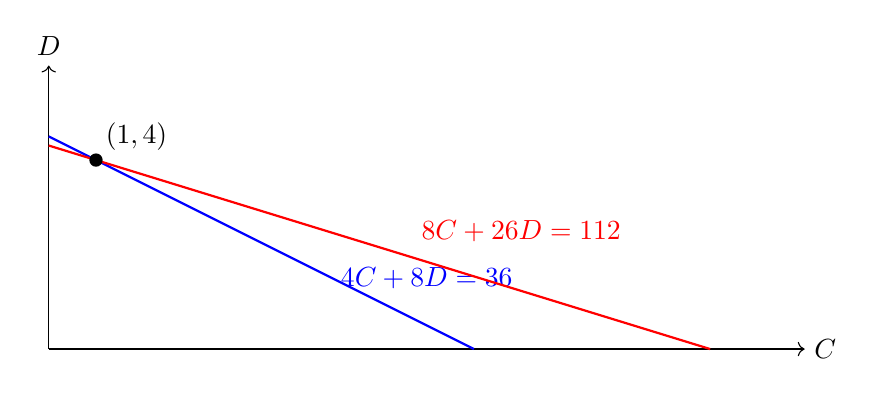
\begin{tikzpicture}[scale=0.6]
    % axes
    \draw[->] (0,0) -- (16,0) node[right] {$C$}; \draw[->] (0,0) -- (0,6)
    node[above] {$D$};

    % line C + 2D = 9
    \draw[blue, thick] (9,0) -- (0,4.5); \node[blue] at (8,1.5) {$4C+8D=36$};

    % line 4C + 13D = 56
    \draw[red, thick] (14,0) -- (0,112/26); \node[red] at (10,2.5) {$8C+26D=112$};

    % intersection point
    \fill (1,4) circle (4pt); \node[above right] at (1,4) {$(1,4)$};
  \end{tikzpicture}
\end{center}

We need to check that $(C,D)=(1,4)$ is a minimum. We could show this with the
second derivative test, but there is also a nice geometric reason why it must
be a minimum. In particular, observe that $f$ is a sum of squares, so it is
bounded below by zero. By considering cross-sections (i.e., freeze one of
either $C$ or $D$ and vary the other), we get an upward-opening parabola in
any direction. So the garph is an upward-opening elliptic paraboloid; i.e., a
bowl-shape, as shown:
\begin{center}
  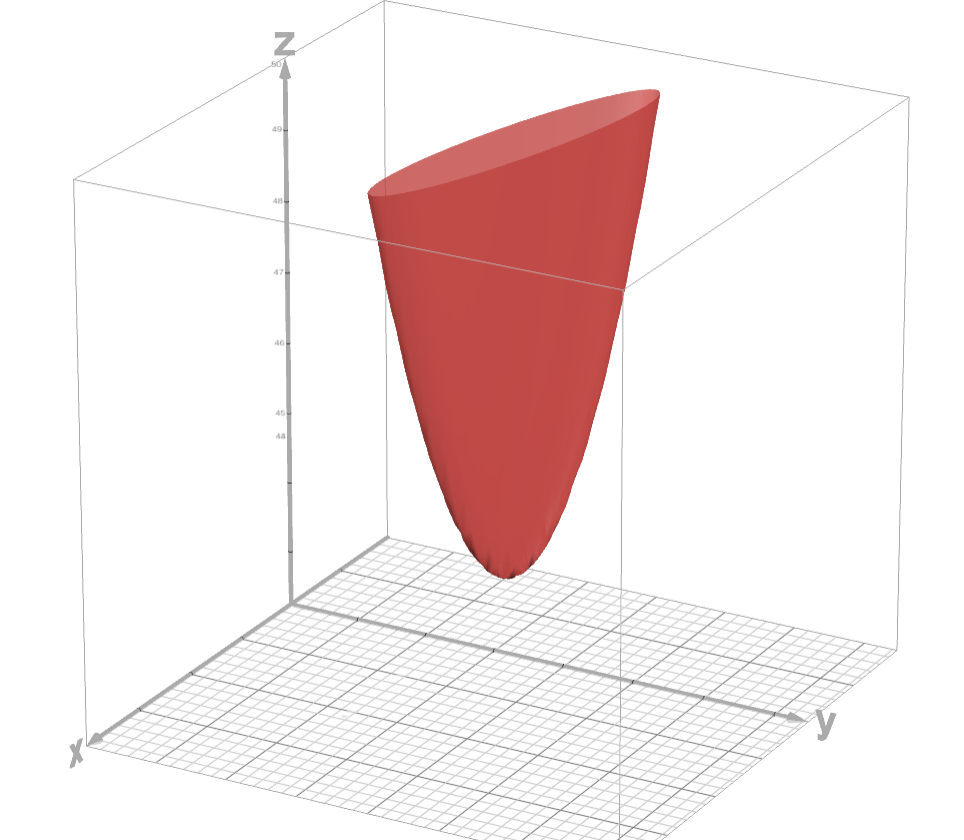
\includegraphics[scale=.2]{images/linear-regression-f}
\end{center}
Hence $f$ has exactly one critical point and the critical point is
the global minimum.

Therefore $f$ is minimized at $(C,D)=(1,4)$. Hence, the best fitting line for
our data is
\begin{equation*}
  y=1+4t,
\end{equation*}
as this line, out of all possible lines, minimizes the sum of squared errors
$e_{1}^{2}+e_{2}^{2}+e_{3}^{2}+e_{4}^{2}$.

\Fl{Approach \#2: Linear Algebra}

There is a compact way to organize these computations using matrices, which
allows us to compute the best fit line without taking any derivatives.

To motivate this, observe that ideally our best-fit line would pass through
all the points, which occurs precisely when $C$ and $D$ satisfy the following
system of equations:
\begin{equation*}
  \left\{ \begin{array}{l@{}l}
      C+0\cdot D=0 \\
      C+1\cdot D=8 \\
      C+3\cdot D=8 \\
      C+4\cdot D=20 \\
    \end{array}\right.
\end{equation*}
This is a system of 4 linear equations in 2 unknowns $(C,D)$. We can write it
in matrix form as

\begin{equation*}
  \underbrace{\begin{bmatrix}
      1&0\\
      1&1\\
      1&3\\
      1&4
    \end{bmatrix}}_{A}
  \underbrace{\begin{bmatrix}
      C\\D
    \end{bmatrix}}_{x}
  =
  \underbrace{\begin{bmatrix}
      0\\8\\8\\20
    \end{bmatrix}}_{b}
\end{equation*}
or more compactly as
\begin{equation*}
  Ax=b.
\end{equation*}

% \begin{remark}
%   More generally, we had data $(t_{1},b_{1}),\ldots,(t_{4},b_{4})$ and our
%   matrices took the form
%   \begin{equation*}
%     A=
%     \begin{bmatrix}
%       1&t_{1}\\
%       1&t_{2}\\
%       1&t_{3}\\
%       1&t_{4}
%     \end{bmatrix},
%     \quad
%     x =
%     \begin{bmatrix}
%       C\\D
%     \end{bmatrix}
%     \quad \text{and} \quad
%     b=
%     \begin{bmatrix}
%       b_{1}\\b_{2}\\b_{3}\\b_{4}
%     \end{bmatrix}.
%   \end{equation*}
% \end{remark}

The bad news is that there is no choice of $C$ and $D$ for which this equation
is true (because the data points \textbf{do not lie on a line}).

So
instead we want $Ax$ be as close as possible to $b$; that is
\begin{equation*}
  Ax\approx b.
\end{equation*}
Since $\mathbf{e}= b-Ax$, we want
\begin{equation*}
  \mathbf{e} =
  \begin{bmatrix}
    e_{1}\\e_{2}\\e_{3}\\e_{4}
  \end{bmatrix}
  \approx 0.
\end{equation*}
So we want the vector $\mathbf{e}$ to be as tiny as possible. By minimizing
$e_{1}^{2}+e_{2}^{2}+e_{3}^{2}+e_{4}^{2}$, we will also simultaneously
minimize $\sqrt{e_{1}^{2}+e_{2}^{2}+e_{3}^{2}+e_{4}^{2}}$, which is the length
of $\mathbf{e}$. This gives a geometric intepretation of our goal: finding the
values of $C$ and $D$ which give the best fit line $y=C+Dt$ to our data is
equivalent to finding the values of $C$ and $D$ which \textbf{minimize the the
  length of the residual vector} $\mathbf{e}$.

To do this, we multiply both sides of $Ax=b$ by
\begin{equation*}
  A^{\top}=
  \begin{bmatrix}
    1&1&1&1\\
    0&1&3&4
  \end{bmatrix}.
\end{equation*}
This yields the following system of equations, called the \demph{normal equations}:
\begin{equation}\label{eq:normal-equations}
  A^{\top}Ax=A^{\top}b.
\end{equation}
Writing out \cref{eq:normal-equations}, we get
\begin{equation*}
  \begin{bmatrix}
    4&8\\
    8&26
  \end{bmatrix}
  \begin{bmatrix}
    C\\D
  \end{bmatrix}
  =
  \begin{bmatrix}
    36\\112
  \end{bmatrix}
\end{equation*}
or equivalently,
\begin{equation*}
  \left\{ \begin{array}{l@{}l} 4C+8D=36 \\ 8C+26D=112 \end{array}\right.
\end{equation*}
This system is the normal equations. Observe that it is the same as
\cref{eq:31} and has the same solution: $(C,D)=(1,4)$, which is the minimizer
of $\norm{\mathbf{e}}^{2}= e_{1}^{2}+\ldots+e_{4}^{2}$.


\newpage
\section{2026-05-04 | Week 16 | Lecture 34}
\textit{Based on chapters 12.1 and 12.2 in the textbook}

Suppose we are given data $(t_{i},b_{i})$, $i=1,\ldots,n$. The \demph{simple
  linear regression problem} is to find the line $y=C+Dt$ which best fits the
data.

In this problem, we understand the ``line of best fit'' to the be the line
$y=C+Dt$ in which $C$ and $D$ are chosen such that the \demph{sum of squared
  errors}
\begin{equation*}
  e_{1}^{2}+\ldots+e_{n}^{2}
\end{equation*}
is minimized. Here, the $e_{i}$'s the the entries of the \demph{residual
  vector} $e$, defined as:
\begin{equation*}
  \mathbf{e}=
  \begin{bmatrix}
    e_{1}\\\vdots\\e_{n}
  \end{bmatrix}
  = b-Ax
\end{equation*}
where
\begin{equation*}
  b =
  \begin{bmatrix}
    b_{1}\\b_{2}\\\vdots\\b_{n}
  \end{bmatrix}
  \quad \text{and} \quad
  A =
  \begin{bmatrix}
    1&t_{1}\\
    1&t_{2}\\
    \vdots&\vdots\\
    1&t_{n}
  \end{bmatrix}
\end{equation*}
In the last lecture, we saw that minimizing the sum of squared errors is
equivalent to minimizing the length of the vector $\mathbf{e}$.


We also saw two appraoches to finding the best values for $C$ and $D$. The
first approach involved calculus. The second approach used linear algebra,
which which what we'll focus on today. Recall the following definition:

\begin{definition}[Normal equations]
  The \demph{normal equations} are
  \begin{equation*}
    A^{\top}Ax= A^{\top}b.
  \end{equation*}
\end{definition}

The linear algebra approach is easy to summarize: to find the best fit line
$y=C+Dt$, set up the equation $A^{\top}Ax=A^{\top}b$ and solve it for $x=
  \begin{bmatrix}
    C\\D
  \end{bmatrix}$.

\begin{example}
  Suppose we have the following data:
  
  \begin{minipage}{0.35\textwidth}
    \centering
    \begin{tabular}{c|c}
      $t$ & $y$ \\
      \hline
      $-2$ & $0$ \\
      $-1$ & $0$ \\
      $0$ & $1$ \\
      $1$ & $1$ \\
      $2$ & $3$ \\
    \end{tabular}
  \end{minipage}
  \quad \quad
  \begin{minipage}{0.4\textwidth}
    \centering
    \begin{tikzpicture}[x=1cm,y=1cm]
      % axes
      \draw[->] (-2.4,0) -- (2.4,0) node[right] {$t$};
      \draw[->] (0,-0.2) -- (0,3.4) node[above] {$y$};

      % x-axis ticks
      \foreach \x in {-2,-1,0,1,2}
      \draw (\x,0.08) -- (\x,-0.08) node[below] {\x};

      % y-axis ticks
      \foreach \y in {1,2,3}
      \draw (0.08,\y) -- (-0.08,\y) node[left] {\y};

      % data points
      \fill (-2,0) circle (2pt);
      \fill (-1,0) circle (2pt);
      \fill (0,1) circle (2pt);
      \fill (1,1) circle (2pt);
      \fill (2,3) circle (2pt);
    \end{tikzpicture}
  \end{minipage}
  \Fl{Question:} Find the best-fitting line $y=C+Dt$.


  \Fl{Solution:} Consider the equation
  \begin{equation*}
    Ax = b
  \end{equation*}
  where
  \begin{equation*}
    A =
    \begin{bmatrix}
      1&-2\\
      1&-1\\
      1&0\\
      1&1\\
      1&2
    \end{bmatrix},
    \quad
    x =
    \begin{bmatrix}
      C\\D
    \end{bmatrix},
    \quad \text{and} \quad
    b =
    \begin{bmatrix}
      0\\0\\1\\1\\3
    \end{bmatrix}.
  \end{equation*}
  Since the data points don't lie on a line, there is no solution (i.e., no
  values of $C$ and $C$ which make this equation true). So instead, we set up
  the normal equations
  \begin{equation*}
    A^{\top}Ax = A^{\top}b
  \end{equation*}
  which are
  \begin{equation*}
    \begin{bmatrix}
      1&1&1&1&1\\
      -2&-1&0&1&2
    \end{bmatrix}
    \begin{bmatrix}
      1&-2\\1&-1\\1&0\\1&1\\1&2
    \end{bmatrix}
    \begin{bmatrix}
      C\\D
    \end{bmatrix}
    =
    \begin{bmatrix}
      1&1&1&1&1\\
      -2&-1&0&1&2
    \end{bmatrix}
    \begin{bmatrix}
      0\\0\\1\\1\\3
    \end{bmatrix}.
  \end{equation*}
  This simplifies to
  \begin{equation*}
    \begin{bmatrix}
      5&0\\
      0&10
    \end{bmatrix}
    \begin{bmatrix}
      C\\D
    \end{bmatrix}
    =
    \begin{bmatrix}
      5\\7
    \end{bmatrix}
  \end{equation*}
  From this we conclude that $C=1$ and $D=7/10$. Hence, our best-fitting line
  is $y=1+.7t$.

  \begin{center}
    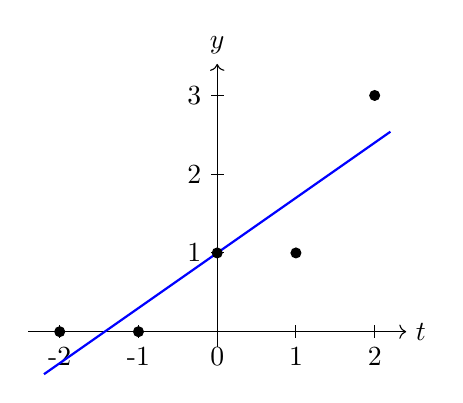
\begin{tikzpicture}[x=1cm,y=1cm]
      % axes
      \draw[->] (-2.4,0) -- (2.4,0) node[right] {$t$};
      \draw[->] (0,-0.2) -- (0,3.4) node[above] {$y$};

      % x-axis ticks
      \foreach \x in {-2,-1,0,1,2}
      \draw (\x,0.08) -- (\x,-0.08) node[below] {\x};

      % y-axis ticks
      \foreach \y in {1,2,3}
      \draw (0.08,\y) -- (-0.08,\y) node[left] {\y};

      % regression line
      \draw[blue, thick, domain=-2.2:2.2] plot (\x, {1 + 0.7*\x});

      % data points
      \fill (-2,0) circle (2pt);
      \fill (-1,0) circle (2pt);
      \fill (0,1) circle (2pt);
      \fill (1,1) circle (2pt);
      \fill (2,3) circle (2pt);
    \end{tikzpicture}
  \end{center}
\end{example}


\begin{example}
  \Fl{Question:} Find the best fitting line to the data
  \begin{center}
    \begin{tabular}{c|c}
      $t$ & $y$ \\
      \hline
      $0$ & $1$ \\
      $1$ & $2$ \\
      $2$ & $2$ \\
      $3$ & $4$ \\
      $4$ & $5$ \\
    \end{tabular}
  \end{center}
  \Fl{Solution:} We have
  \begin{equation*}
    A =
    \begin{bmatrix}
      1&0\\
      1&1\\
      1&2\\
      1&3\\
      1&4\\
    \end{bmatrix},
    \quad
    b =
    \begin{bmatrix}
      1\\2\\2\\4\\5
    \end{bmatrix}
    \quad \text{and} \quad 
    x =
    \begin{bmatrix}
      C\\D
    \end{bmatrix}.
  \end{equation*}
  Therefore the normal equations $A^{\top}Ax=A^{\top}b$ are
  \begin{equation*}
    \begin{bmatrix}
      5&10\\
      10&30
    \end{bmatrix}
    \begin{bmatrix}
      C\\D
    \end{bmatrix}
    =
    \begin{bmatrix}
      14\\38
    \end{bmatrix}
  \end{equation*}
  or equivalently
  \begin{equation*}
    \left\{ \begin{array}{l@{}l} 5C+10D=14 \\10C+30D=38  \end{array}\right.
  \end{equation*}
  Solving this system gives $C=.8$ and $D=1$. Therefore the best-fit line $y=C+Dt$ is 
  \begin{equation*}
    y = .8+t.
  \end{equation*}
\end{example}


\begin{theorem}
  The values $C$ and $D$ which minimize $e_{1}^{2}+\ldots+e_{n}^{2}$, are
  given by the solution $x=
  \begin{bmatrix}
    C\\D
  \end{bmatrix}
  $ to the normal equations
  \begin{equation*}
    A^{\top}Ax=A^{\top}b,
  \end{equation*}
  where
  \begin{equation*}
    A =
    \begin{bmatrix}
      1&t_{1}\\
      1&t_{2}\\
      \vdots&\vdots\\
      1&t_{n}\\
    \end{bmatrix}
    \quad \text{and} \quad
    b =
    \begin{bmatrix}
      b_{1}\\b_{2}\\\vdots \\b_{n}
    \end{bmatrix}
  \end{equation*}
  % In particular, the solution is
  % \begin{equation*}
  %   x=(A^{\top}A)^{-1}A^{\top}b
  % \end{equation*}
  % and we call it the \demph{least squares solution} to $Ax=b$.
\end{theorem}
\begin{proof}
  I tried to explain this geometrically. If $x$ is the solution to the normal
  equations, then $e=b-Ax$ is orthogonal to $\text{CS}(A)$, which guarantees
  that the the length of the residual vector is minimized.
\end{proof}


% Essential to the above approach is the following proposition, which implies
% that as long as $A$ has linearly independent columns (always the case in
% problems like this) then normal equations always have a unique solution:

% \begin{proposition}
%   If $A$ has linearly independent columns, then $A^{\top}A$ is invertible.
% \end{proposition}
% \begin{proof}
%   Suppose $x\in \ker(A^{\top}A)$. Then $A^{\top}Ax=0$. Multipying by
%   $x^{\top}$ on the left implies
%   \begin{equation*}
%     x^{\top}A^{\top}Ax=0.
%   \end{equation*}
%   Since $x^{\top}A^{\top}Ax=(Ax)^{\top}(Ax)=\norm{Ax}$, it follows that
%   $\norm{Ax}=0$. Therefore
%   \begin{equation*}
%     Ax=0.
%   \end{equation*}
%   Therefore, since $A$ has linearly independent columns, $x=0$. We have shown
%   that $\ker(A^{\top}A)=\left\{0\right\}$. Therefore $A^{\top}A$ is
%   invertible.
% \end{proof}
\end{document}